\documentclass[journal]{new-aiaa}
%\documentclass[conf]{new-aiaa} for conference papers
\usepackage{AAS_packages}
% \usepackage[utf8]{inputenc}

% \usepackage[version=4]{mhchem}
% \usepackage{longtable,tabularx}
% \setlength\LTleft{0pt} 

\newcommand{\todo}[1]{\vspace{5 mm}\par \noindent
\marginpar{\textsc{ToDo}} \framebox{\begin{minipage}[c]{0.95
\textwidth} \tt #1 \end{minipage}}\vspace{5 mm}\par}
%\newcommand{\todo}[1]{}
\DeclareMathOperator*{\argmin}{arg\,min}

\title{Bayesian Shape Reconstruction and Optimal Guidance for Autonomous Landing on Asteroids}

% TODO Think about adding current affiliation as a note, need to ask company
\author{Shankar Kulumani \footnote{PhD, Mechanical and Aerospace Engineering, \href{mailto:skulumani@gwu.edu}{skulumani@gwu.edu}}
and
Taeyoung Lee \footnote{Associate Professor, Mechanical and Aerospace Engineering, \href{mailto:tylee@gwu.edu}{tylee@gwu.edu}}}
\affil{The George Washington University, Washington, DC, 20052}

\begin{document}

\maketitle

\begin{abstract}
    Constructing of the precise shape of an asteroid is critical for spacecraft operations, as the gravitational potential is determined by spatial mass distribution.
    For example, the standard method of determining the gravitational potential of an asteroid, through the use of a polyhedron potential model, is directly dependent on the shape model.
    Furthermore, safe landing or close-proximity operations requires accurate knowledge of the surface topology. 
    The typical approach to shape determination requires a prolonged ``mapping'' phase of the mission over which extensive measurements are collected and transmitted for Earth-based processing.
    This paper presents a set of approaches to explore an unknown asteroid with onboard calculations, and to land on its surface area selected in an optimal fashion. 
    The main motivation is to avoid the extended period of mapping phase or preliminary ground observations that are commonly required in spacecraft mission around asteroids. 
    First, range measurements from spacecraft to the surface are used to incrementally correct an initial shape estimate according to the Bayesian framework. 
    Then, an optimal guidance scheme is proposed to control the vantage point of the range sensor to construct a complete 3D model of the asteroid shape. 
    This shape model is then used in a nonlinear controller to track a desired trajectory about the asteroid.
    Finally, a multi resolution approach is presented to construct a higher fidelity shape representation in a specified location while avoiding the inherent burdens of a uniformly high resolution mesh. 
    This approach enables for an accurate shape determination around a potential landing site.
    We demonstrate this approach using several radar shape models of asteroids and provide a full dynamic simulation about asteroid 4769 Castalia.
\end{abstract}

\section*{Nomenclature}

\noindent(Nomenclature entries should have the units identified)
\noindent{Add elements}
% {\renewcommand\arraystretch{1.0}
% \noindent\begin{longtable*}{@{}l @{\quad=\quad} l@{}}
% $A$  & amplitude of oscillation \\
% $a$ &    cylinder diameter \\
% $C_p$& pressure coefficient \\
% $Cx$ & force coefficient in the \textit{x} direction \\
% $Cy$ & force coefficient in the \textit{y} direction \\
% c   & chord \\
% d$t$ & time step \\
% $Fx$ & $X$ component of the resultant pressure force acting on the vehicle \\
% $Fy$ & $Y$ component of the resultant pressure force acting on the vehicle \\
% $f, g$   & generic functions \\
% $h$  & height \\
% $i$  & time index during navigation \\
% $j$  & waypoint index \\
% $K$  & trailing-edge (TE) nondimensional angular deflection rate\\
% $\Theta$ & boundary-layer momentum thickness\\
% $\rho$ & density\\
% \multicolumn{2}{@{}l}{Subscripts}\\
% cg & center of gravity\\
% $G$ & generator body\\
% iso	& waypoint index
% \end{longtable*}}




\section{Introduction}
% Motivation for missions/studying asteroids
Small solar system bodies, such as asteroids and comets, continue to remain a focus of scientific study.
The small size of these bodies prevents the formation of large internal pressures and temperatures which helps to preserve the early chemistry of the solar system.
This insight offers additional detail into the formation of the Earth and also of the probable formation of other extrasolar planetary bodies.
Of particular interest are those near-Earth asteroids (NEA) which inhabit heliocentric orbits in the vicinity of the Earth. 
These easily accessible bodies provide attractive targets to support space industrialization, mining operations, and scientific missions.
In spite of the significant interest, and the extensive research by the community, the operation of spacecraft near small bodies remains a challenging problem.

% dynamics are difficult around asteroids
The dynamic environment around asteroids is strongly perturbed and challenging for analysis and mission operations~\cite{scheeres2012}.
Due to their low mass, which in turn causes a low gravitational attraction, asteroids may have irregular shapes.
Furthermore, asteroids may also have a chaotic spin state due to the absorption and emittance of solar radiation~\cite{rubincam2000}.
As a result, approaches utilizing an inverse square gravitational model do not capture the  true dynamic environment.
In addition, the vast majority of asteroids are difficult to track and characterize using ground based sensors.
Due to their small size, frequently with a maximum radius less than \SI{1}{\kilo\meter}, and low albedo, the reflected energy of these asteroids is insufficient for reliable detection or tracking.
Therefore, the dynamics model of the asteroid is relatively coarse prior to in situ measurements from a dedicated spacecraft.
As a result, any spacecraft mission to an asteroid must include the ability to update the dynamic model given in situ measurements and remain robust to unmodelled forces.

Another key dynamic consideration is the coupling between rotational and translational states around the asteroid.
The coupling is induced due to the different gravitational forces experienced on various portions of the spacecraft. 
The effect of the gravitational coupling is related to the ratio of the spacecraft size and orbital radius~\cite{hughes2004}.
For operations around asteroids, the ratio is relatively large which causes a much larger coupling between the translational and rotational states.
References~\citenum{elmasri2005} and~\citenum{sanyal2004a} investigated the coupling of an elastic dumbbell spacecraft in orbit about a central body, but only considered the case of a spherically symmetric central body.
Furthermore, the spacecraft model is assumed to remain in a planar orbit.
As a result, these developments are not directly applicable to motion about an asteroid, which experiences highly non-Keplerian motion.
Reference~\citenum{misra2015b} investigated the effect of coupled motion on long term trajectories around asteroids.
However, the analysis only considered a second order spherical harmonic gravitational potential model. 
Therefore, these results are only valid when far from the asteroid surface and will diverge when used within the Brillouin sphere.

% Gravity model is important and dependent on shape
An accurate gravitational potential model is critical for performing low altitude and/or surface operations around asteroids.
Due to the irregular shape, trajectories will pass within the Brillouin sphere, where the typical spherical harmonic model diverges from the true gravitational potential.
The standard approach for asteroid missions is to compute the gravitational potential using a polyhedron potential model~\cite{werner1996}.
The polyhedron potential model provides the exact gravitational potential, and subsequently the gravitational acceleration, for a given triangular faceted shape model of an asteroid.
The method provides the exact potential at any point outside the body for a given shape model.
As a result, the accuracy of the gravitational potential is primarily dependent on the accuracy with which the shape model represents the true surface.
A high fidelity shape, which necessarily has many vertices and faces, is required for an accurate computation of the gravitational acceleration and enabling low altitude operations.

% Challenges involved in operation near asteroids (gravity, shape, distance)
% generating the shape from the ground is difficult
Prior to the arrival of a spacecraft at an asteroid, Earth-based sensors are used to characterize the body.
Using both optical and radar sensors allows for the precise orbit of the asteroid to be determined.
Another vital task is the determination of the asteroid shape from radar data~\cite{hudson1994,busch2011}.
This is a challenging problem as it requires the simultaneous estimation of the asteroid spin state and shape.
Furthermore, determining the shape from radar is currently the only Earth-based technique that can produce detailed three-dimensional shape information of near-Earth objects~\cite{greenberg2015}.
The current approach is based on an estimation scheme which iteratively perturbs a shape to match given radar data.
This computationally intensive approach is only able to capture the gross size and shape and is unable to capture the small surface features of the asteroid.
Frequently, only a coarse model is possible from the ground and an accurate shape must be determined only after a spacecraft has rendezvoused with the asteroid.
As a result, upon arrival the gravitational environment near the asteroid is poorly modeled as the shape of the asteroid is not accurate.
Therefore, the polyhedron potential model is not appropriate immediately upon arrival but rather only after the shape has been determined.

% on arrival spacecraft spend long periods mapping, and depending on mission this might be unallocable
On approach to an asteroid, spacecraft navigation and guidance is primarily based on ground measurements.
After arrival, a spacecraft will generally spend months or years in a mapping mission phase~\cite{kubota2003,cole1998}.
During this period, spacecraft sensors, such as on board optical telescopes or Light radio Detection and Ranging (LIDAR), are used to characterize the asteroid.
The resulting imagery and range data is transmitted to the ground and the resulting asteroid shape and motion is estimated. 
During this mapping phase the spacecraft must remain in a quiescent state devoted entirely to mapping the surface.
Depending on the mission type, this long period of mapping is crucial to the mission, such as sample collection~\cite{gates2015}. 
However, other missions, such as asteroid mitigation, may be severely limited by the time and ground resources required to generate a surface shape.
Furthermore, the long distances involved necessitate on-board autonomy to enable to spacecraft to operate without ground communications.
Similarly, during landing the spacecraft will require the ability to sense and model the surface topography in order to safely land in an unknown environment.
The dependency on expensive ground-based shape reconstruction techniques limits the ability of spacecraft to autonomously operate at asteroids.
Mitigation of this ground based surface modeling will greatly expand the range of missions possible.

% TODO Reduce some of these paragraphs since they're wordy
% we want to generate the shape in real time and then use this shape for updated and better control
This paper presents three techniques to explore an asteroid without need for an extended period of mapping phase or ground based measurements. 
First, we develop a method to compute the surface shape of an asteroid from onborad range measurements.
Assuming that a meshed model of an initial estimate, such as an ellipsoidal shape, is available, the radius of any vertex in the measured area is adjusted according to the measurements. 
This is completed in a stochastic fashion where the degree of confidence in the current shape is compared with the level of measurement noise. 
Our approach is able to operate in real time and incrementally update the shape model of an asteroid as new range measurements are collected.
This approach allows for the shape to be continually updated as range measurements are used to locally modify the shape estimate.
This technique is verified by numerical examples of shape construction for asteroids Geographos and Golevka. 

Next, we present an optimal guidance scheme to construct a complete and accurate shape model of an asteroid. 
The motivation is to actively control the relative position of the spacecraft such that the range sensor covers the surface area from every perspective. 
Utilizing the stochastic formulation of the above shape construction method, this is addressed by an optimization to find the pose of the spacecraft that minimizes the degree of uncertainties in the shape model. 

Finally, we consider the scenario of landing on the surface of an asteroid. 
Once a complete shape model is constructed, we study a landing site selection problem. 
For safety concern, the area with higher slope is excluded. 
Within the low slope region, a landing site is selected to minimize a control cost subtracted by a measure of scientific interests. 
Once the landing site is selected, the nearby area is mapped with a higher resolution to create a detailed topological map.  
The proposed multi resolution mapping yields a high fidelity map without the computational burden of a uniformly high resolution mesh.  

The optimal guidance and multi resolution mapping schemes are illustrated by dynamic simulation of landing on the asteroid Castalia. 
During this simulation, This updated shape model is then used to in a nonlinear controller to track a desired state trajectory for the dynamics of a rigid body spacecraft.
The dynamics are developed on the nonlinear manifold of rigid body motions, namely the special Euclidean group.
This formulation is based on an intrinsic geometric description of the motion and accurately captures the coupling between orbit and attitude dynamics. 

% our approach for paper. Real time method to update asteroid shape model and use updated model in closed loop control

% Benefits and contribution of our approach
In short, this paper presents a method to incrementally update the shape  model of an asteroid from range measurements. 
Our approach alleviates the need for a dedicated mapping phase as the spacecraft is able to update its shape model in real time and without expensive computations.
This type of approach allows for the spacecraft to maneuver and land on the asteroid immediately upon arrival rather than spending several months mapping the surface.

\section{Problem Formulation}\label{sec:problem}

In this paper, we consider the motion of a dumbbell model of spacecraft around an asteroid.
The dumbbell model captures the important interactions of the coupling between orbital and attitude dynamics.
The dumbbell is defined by two spherical masses of radius \( r_1, r_2 \in \R \) with masses \( m_1, m_2 \in  \R\).
The masses are separated by a massless rod of length \( l \) and attached to the centers of each mass.
\Cref{fig:dumbbell_sc} shows the model and associated parameters.
\begin{figure}[htbp]
    \centering
    %% helper macros

\newcommand\pgfmathsinandcos[3]{%
  \pgfmathsetmacro#1{sin(#3)}%
  \pgfmathsetmacro#2{cos(#3)}%
}
\newcommand\LongitudePlane[3][current plane]{%
  \pgfmathsinandcos\sinEl\cosEl{#2} % elevation
  \pgfmathsinandcos\sint\cost{#3} % azimuth
  \tikzset{#1/.style={cm={\cost,\sint*\sinEl,0,\cosEl,(0,0)}}}
}
\newcommand\LatitudePlane[3][current plane]{%
  \pgfmathsinandcos\sinEl\cosEl{#2} % elevation
  \pgfmathsinandcos\sint\cost{#3} % latitude
  \pgfmathsetmacro\yshift{\cosEl*\sint}
  \tikzset{#1/.style={cm={\cost,0,0,\cost*\sinEl,(0,\yshift)}}} %
}

\newcommand\DrawLongitudeCircle[4][1]{
\LongitudePlane{\angEl}{#2}
\tikzset{current plane/.prefix style={scale=#1}}
% angle of "visibility"
\pgfmathsetmacro\angVis{
atan(sin(#2)*cos(\angEl)/sin(\angEl))} %
\draw[shift={(#3, #4)}][current plane]
(\angVis:1) arc (\angVis:\angVis+180:1);
\draw[shift={(#3, #4)}][current plane,dashed]
(\angVis-180:1)arc(\angVis-180:\angVis:1);
}
\newcommand\DrawLatitudeCircle[4][1]{
\LatitudePlane{\angEl}{#2}
\tikzset{current plane/.prefix style={scale=#1}}
\pgfmathsetmacro\sinVis{
sin(#2)/cos(#2)*sin(\angEl)/cos(\angEl)}
% angle of "visibility"
\pgfmathsetmacro\angVis{
asin(min(1,max(\sinVis,-1)))}
\draw[shift={(#3, #4)}][current plane]
(\angVis:1) arc (\angVis:-\angVis-180:1);
\draw[shift={(#3, #4)}][current plane,dashed]
(180-\angVis:1)arc(180-\angVis:\angVis:1);
}

%% document-wide tikz options and styles

\tikzset{%
  >=latex, % option for nice arrows
  inner sep=0pt,%
  outer sep=2pt,%
  mark coordinate/.style={inner sep=0pt,outer sep=0pt,minimum size=3pt,
    fill=black,circle}%
}

\tikzsetnextfilename{dumbbell}
\begin{tikzpicture} % "THE GLOBE" showcase

\def\R{2} % sphere radius
\def\angEl{35} % elevation angle
\def\angAz{-105} % azimuth angle
\def\length{4} % distance from COM to M_1
\def\opacity{0.2}

% centers of the masses
\coordinate (m1) at (\length, 0);
\coordinate (m2) at (-\length, 0);

\draw [ thick, dashed, -Latex] (m2) -- ($ (m1) + (3, 0) $) node [below right] {$b_1$};
\draw [thick, dashed, -Latex] (0, 0) -- (0, \R) node [above right] {$b_2$};
% TODO Make a macro to draw a sphere at a sphefic point
\filldraw[ball color=blue, opacity=\opacity] (m1) circle (\R);
\foreach \t in {-45, 0, 45} { \DrawLatitudeCircle[\R]{\t}{\length}{0} }
\foreach \t in {-30, -60,...,-150} { \DrawLongitudeCircle[\R]{\t}{\length}{0} }

\filldraw[ball color=blue, opacity=\opacity] (m2) circle (\R);
\foreach \t in {-60,-30,...,60} { \DrawLatitudeCircle[\R]{\t}{-\length}{0} }
\foreach \t in {-5,-35,...,-175} { \DrawLongitudeCircle[\R]{\t}{-\length}{0} }

% draw from origin to center of m1
\draw[thick,-Latex] node [below right] {$\zeta$} (0, 0) --  (m1);
\draw[thick,-Latex] (m1) -- ++(30:\R) node [above right] {$\eta$};

% draw the radiaii of each mass
% \draw[thick,-Latex] (m1) -- ++(130:\R) node [above right] {$r_1$};

\end{tikzpicture}


    \caption{Dumbbell Model of Rigid Spacecraft\label{fig:dumbbell_sc}}
\end{figure}
Without loss of generality, we define body fixed frames for both the spacecraft and asteroid, which are aligned with the principle axes of each body and originate at their respective center of mass. 
The spacecraft body fixed frame is centered at the center of mass of the vehicle.
The \( b_1 \)  axis is aligned with the connecting rod and directed along the axis of symmetry.
The \( b_2, b_3 \) axes span the plane orthogonal to the axis of symmetry of the dumbbell.
The distance from the center of mass to each spherical mass is defined as
\begin{align}\label{eq:dumbbell_mass_distances}
    l_1 &= \frac{m_2}{m_1 + m_2} l, \\
    l_2 &= l - l_1.
\end{align}
The asteroid is modeled as a constant density polyhedron with constant, and known, spin about its maximum moment of inertia. 
The axes of the body fixed frame for the asteroid are denoted by $\{f_1,f_2,f_3\}$. 
We also define the inertial frame, whose axes are denoted by $\{e_1,e_2,e_3\}$. 

The kinematics of the dumbbell and asteroid are described in the inertial frame by
\begin{itemize}
    \item \( \vc{x}\in\Re^3 \) - the position of the center of mass of the  spacecraft represented in the inertial frame, \( \vc{e}_i\),
    \item \( R\in\SO \) - the rotation matrix which transforms vectors defined in the spacecraft fixed frame, \( \vc{b}_i \), to the inertial frame, \( \vc{e}_i \),
    \item \( \vc{\Omega}\in\Re^3 \) - the angular velocity of the spacecraft body fixed frame relative to the inertial frame and represented in the dumbbell body fixed frame, \( \vc{b}_i \), and
    \item \( R_A\in \SO \) - the rotation matrix which transforms vectors defined in the asteroid fixed frame, \( \vc{f}_i \), to the inertial frame, \( \vc{e}_i \).
\end{itemize}
In this work, we assume that the asteroid is much more massive than the spacecraft and its motion is not affected by that of the spacecraft.
This assumption allows us to treat the motion of the vehicle independently from that of the asteroid. 

\subsection{Spacecraft Dynamic Model}

\todo{Define every variable, $m_1,m_2,\rho_1,\ldots$. }

Using Hamilton's principle one can derive the inertial equations of motion of the dumbbell spacecraft~\cite{kulumani2017b} as
\begin{align}
    \dot{\vc{x}} &= \vc{v}, \\
    \parenth{m_1 + m_2} \dot{\vc{v}} &= m_1 R_A \deriv{U}{\vc{z}_1} + m_2 R_A \deriv{U}{\vc{z}_2} + u_f,\label{eq:v_dot} \\
    \dot{R} &= R S(\vc{\Omega}) , \\
    J \dot{\vc{\Omega}} + \vc{\Omega} \times J \vc{\Omega} &= \vc{M}_1 + \vc{M}_2 + u_m.
\end{align}
The vectors \( \vc{z}_1 \) and \( \vc{z}_2\) define the position of the dumbbell masses in the asteroid fixed frame and are defined as
\begin{align}
    \vc{z}_1 &= R_A^T \parenth{\vc{x} + R \vc{\rho}_1} , \\
    \vc{z}_2 &= R_A^T \parenth{\vc{x} + R \vc{\rho}_2},
\end{align}
where \( \rho_i \) defines the position of each mass in the spacecraft fixed body frame.
The control inputs to the spacecraft are defined by \( u_f, u_m \in \Re^3 \) which define the control force represented in the inertial frame and the control moment represented in the spacecraft frame, respectively.
The standard moment of inertia of the dumbbell model is 
\begin{align}\label{eq:dumbbell_moment_of_inertia}
    J_I = \sum_i^n J_i + m_i \parenth{\vc{\zeta}_i^T \vc{\zeta}_i I - \vc{\zeta}_i \vc{\zeta}_i^T} , 
\end{align}
where \( \vc{\zeta}_i \) is the position of \( m_i \) in the spacecraft fixed frame and the moment of inertia of each sphere is
\begin{align}\label{eq:sphere_moment_of_inertia}
    J_i = \begin{bmatrix} 
        \frac{2}{5} m_i r_i^2 & 0 & 0 \\
        0 & \frac{2}{5} m_i r_i^2 & 0 \\
        0 & 0 & \frac{2}{5} m_i r_i^2 
    \end{bmatrix}.
\end{align}
\Cref{eq:dumbbell_moment_of_inertia} is consistent with the well-known parallel-axis theorem~\cite{greenwood1988}.
We utilize a nonstandard moment of inertia in the equations of motion, \( J_d \in \R^{3 \times 3 } \), which is related to the standard moment of inertia by
\begin{subequations}\label{eq:moi_transformation}
    \begin{align}
        J &= \tr{J_d} I - J_d, \label{eq:moi_ns2s}\\
        J_d &= \frac{1}{2} \tr{J} I - J.\label{eq:moi_s2ns}
    \end{align}
\end{subequations}     
The gravitational moment on the dumbbell \( \vc{M}_i\) is defined as
\begin{align}
    \vc{M}_i = m_i \parenth{S(R_A^T \vc{\rho}_i) R^T \deriv{U}{\vb{z}_i}}.
\end{align}
In the above equations, the gravitational potential is denoted by $U$, which is computed by a polyhedron model as described in the subsequent section. 

%where the polyhedron potential is defined as 
%\begin{align}
    %U(\vc{r}) &= \frac{1}{2} G \sigma \sum_{e \in \text{edges}} \vc{r}_e \cdot \vc{E}_e \cdot \vc{r}_e \cdot L_e - \frac{1}{2}G \sigma \sum_{f \in \text{faces}} \vc{r}_f \cdot \vc{F}_f \cdot \vc{r}_f \cdot \omega_f,
%\end{align}
%and \( \vc{r}_e\) and \(\vc{r}_f \) are the vectors from the spacecraft to any point on the respective edge or face, \( G\) is the universal gravitational constant, and \( \sigma \) is the constant density of the asteroid.
%The position of each mass \(m_i\) of the dumbbell is defined in the dumbbell fixed frame by the vector \(\vb{\rho}_i\). 


\subsection{Polyhedron Potential Model}\label{sec:polyhedron_potential}

% most use a spherical harmonic model or a ellipsoid model but we use a polyhedron model
An accurate gravitational potential model is necessary for the operation of spacecraft about asteroids.
Additionally, a detailed shape model of the asteroid is needed for trajectories passing close to the body.
The classic approach is to expand the gravitational potential into a harmonic series and compute the series coefficients.
However, the harmonic expansion is always an approximation as a result of the infinite order series used in the representation.
Additionally, the harmonic model used outside of the circumscribing sphere is not guaranteed to converge inside the sphere, which makes it unsuitable for trajectories near the surface.

We represent the gravitational potential of the asteroid using a polyhedron gravitation model.
This model is composed of a polyhedron, which is a three-dimensional solid body, that is defined by a series of vectors in the body-fixed frame.
The vectors define vertices in the body-fixed frame as well as planar faces which compose the surface of the asteroid.
We assume that each face is a triangle composed of three vertices and three edges.
As a result, only two faces meet at each edge while three faces meet at each vertex.
Only the body-fixed vectors, and their associated topology, is required to define the exterior gravitational model.
References~\cite{werner1994} and~\cite{werner1996} give a detailed derivation of the polyhedron model.
Here, we summarize the key equations required for implementation.

We define the attraction, gravity gradient matrix, and Laplacian as
\begin{align}
    \nabla U ( \vc{r} ) &= -G \sigma \sum_{e \in \text{edges}} \vc{E}_e \cdot \vc{r}_e \cdot L_e + G \sigma \sum_{f \in \text{faces}} \vc{F}_f \cdot \vc{r}_f \cdot \omega_f \in \R^{3 \times 1} , \label{eq:attraction}\\
    \nabla \nabla U ( \vc{r} ) &= G \sigma \sum_{e \in \text{edges}} \vc{E}_e  \cdot L_e - G \sigma \sum_{f \in \text{faces}} \vc{F}_f \cdot \omega_f \in \R^{3 \times 3}, \label{eq:gradient_matrix}\\
    \nabla^2 U &= -G \sigma \sum_{f \in \text{faces}}  \omega_f \in \R^1 .\label{eq:laplacian}
\end{align}
One interesting thing to note is that both~\cref{eq:face_dyad,eq:edge_dyad} can be precomputed without knowledge of the position of the satellite.
They are both solely functions of the vertices and edges of the polyhedral shape model and are computed once and stored.
Once a position vector \( \vc{r} \) is defined, the scalars given in~\cref{eq:edge_factor,eq:face_factor} can be computed for each face and edge.
Finally,~\cref{eq:potential} is used to compute the gravitational potential on the spacecraft.
The Laplacian, defined in~\cref{eq:laplacian}, gives a simple method to determine if the spacecraft has collided with the body~\cite{werner1996}. 

\section{Bayesian Shape Reconstruction}\label{sec:radius_update}

One of the first tasks for any spacecraft mission to a small body is to generate an estimate of the shape.
We assume that upon arrival at a target body, the spacecraft contains an initial estimate for the shape of the small body.
This shape can be a coarse estimate computed from ground measurements or it can be a triaxial ellipsoid based on the semimajor axes of the asteroid.
Additionally, we assume that the shape estimate is closed and a triangular faceted surface mesh, emulating those used in practice to represent asteroids.
Furthermore, the number of vertices in the estimate can be scaled according to the desired final accuracy or computational capabilities.
In this section, we present a stochastic formulation to update the initial estimate of the shape incrementally based on range measurements from spacecraft. 

\subsection{Range Measurements}

We assume the spacecraft contains a range sensor, such as LIDAR, that allows for the accurate measurement of the relative distance between the spacecraft and asteroid~\cite{zuber1997,zuber2000}.
This type of sensor measures the round-trip time for a pulse of energy to leave the spacecraft, reflect off the surface, and return to a collector on board.
Given the time total time of flight, the distance can be accurately computed using \( d = \frac{\Delta TOF}{2 c} \) where \( c = \SI{2.998e8}{\meter\per\second}\) is the constant speed of light.
Assuming accurate knowledge of the pointing direction of the spacecraft, in the form of the rotation matrix \( R \in \R^{3 \times 3 } \), we can compute a direction from the spacecraft to the measurement location on the surface.
The output of this sensor is a vector, \( \vc{d}_i\in\Re^3 \), defined in the spacecraft fixed frame which gives the direction to a measurement point on the surface. 
Using the state of the asteroid, we can transform this measurement to the asteroid fixed frame using the simple transformation
\begin{align*}
    \vc{p}_i = R_A^T (x+R \vc{d}_i), 
\end{align*}
which is the vector from the origin of the asteroid fixed frame to the surface point of the measurement.

Given many measurements, \( \vc{p}_i \in \R^3 \), of the asteroid surface we can efficiently update our initial shape estimate to that of the true surface.
\Cref{fig:lidar_example} shows asteroid 4769 Castalia and a representation of several LIDAR measurements. 
The spacecraft measures the range between itself and the asteroid surface to several points within the field of view of the sensor. 
These measurements provide a collection of points which lie on the surface of the asteroid, and by combining many points, a so called \textit{point cloud}, allows us to reconstruct the shape.
\begin{figure}
    \centering
    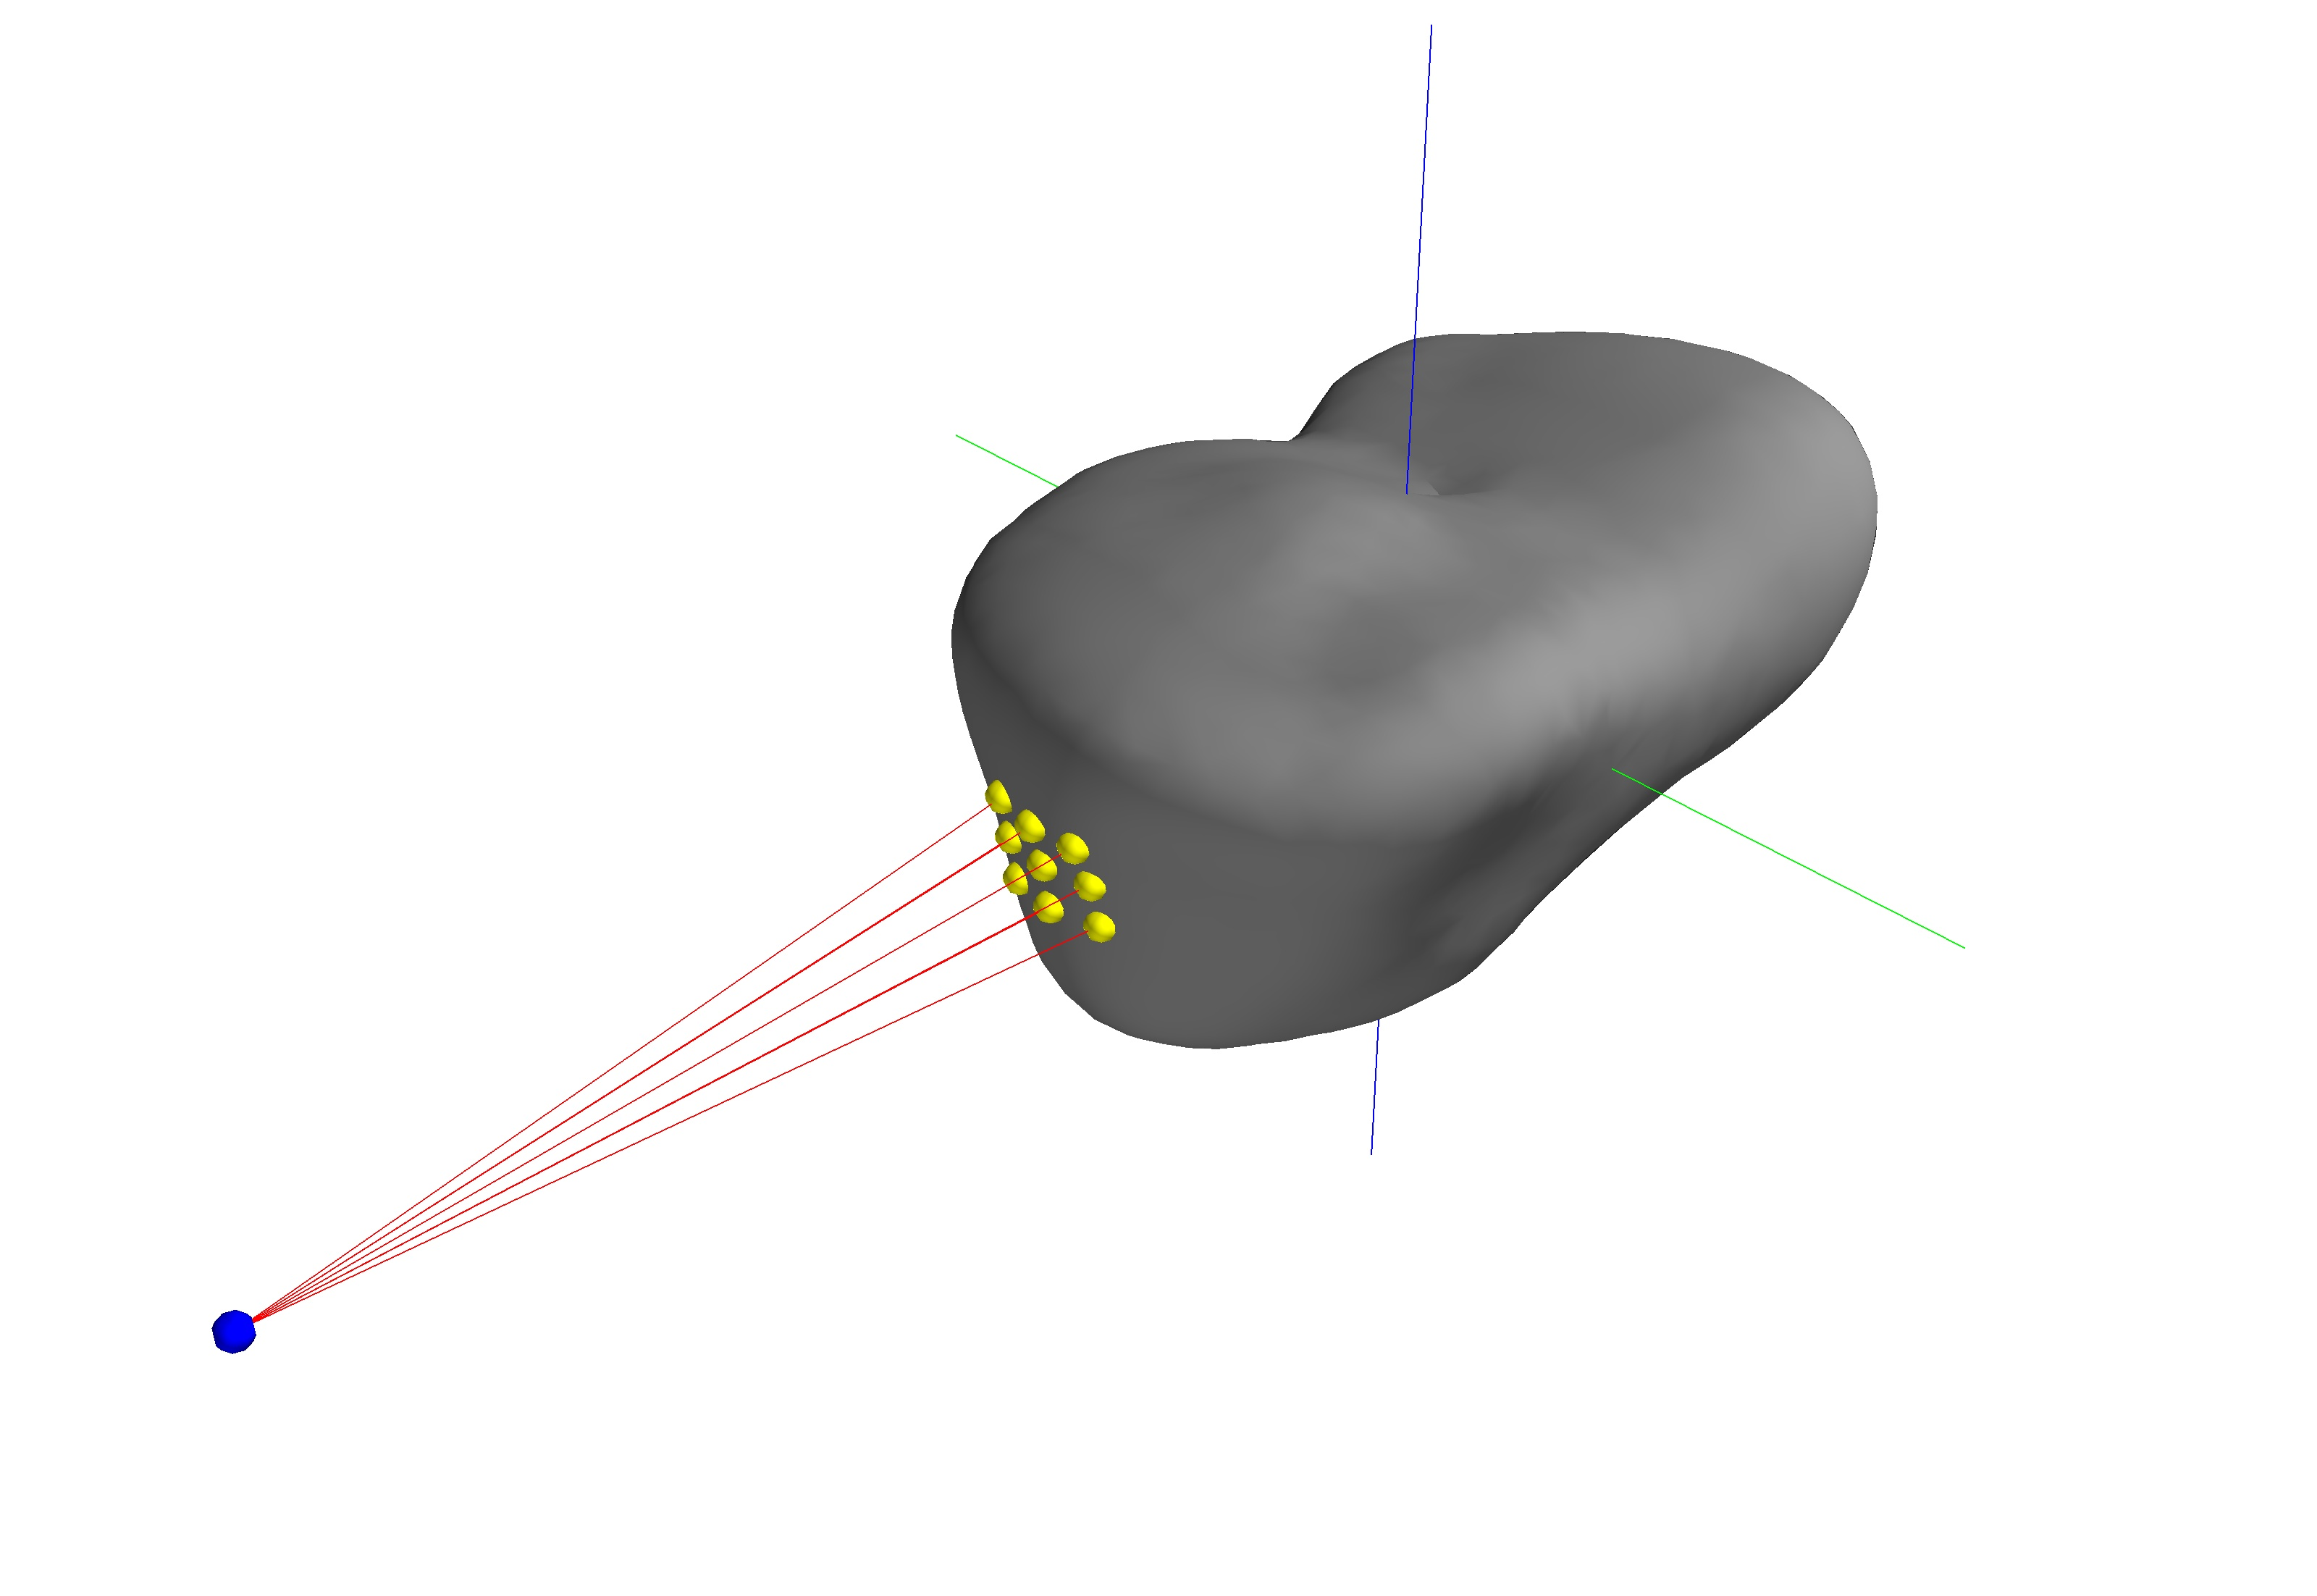
\includegraphics[width=0.75\textwidth]{figures/castalia_raycasting_plot.jpg}
    \caption{Simulated LIDAR measurements of asteroid Castalia~\label{fig:lidar_example}}
\end{figure}

\subsection{Bayesian Shape Update}

Our algorithm applies a probabilistic framework to radially modify each vertex \( \vc{v}_i \in \R^3\) of the shape estimate based on measurement \( \vc{p}_i \in \R^3 \). 
In other words, each vertex from the initial estimate of shape is either stretched or shrunk along its radial direction, without any rotation. 
This framework is reasonable assuming that both of the initial estimate and the actual shape does not have any hole. 
This approach alleviates much of complexity of incorporating new vertices or surface triangulation common in surface reconstruction methods~\cite{berg2008}.
This implies that the total number of vertices of the shape model is fixed.
However, additional detail, in the form of additional vertices, is possible by using standard mesh subdivision algorithms~\cite{orourke1998}, which is discussed in the subsequent section for multi resolution mapping.

The proposed scheme follows a Bayesian estimation scheme, where the degree of confidence in the current estimate is compared with that of new measurements. 
More specifically, the radial distance of each vertex, \( v_i = \norm{\vc{v}_i}\), is assumed to be distributed according to the Gaussian distribution
\begin{align*}
    v_i \sim \mathcal{N}(r_i, w_i^2)
\end{align*}
where \( r_i \) is the initial estimate of the radial distance of vertex \( \vc{v}_i\) and \( w_i \) is the initial variance, or confidence, in the radial distance.

In order to reduce the computational demands, which are typical in point cloud applications, we do not update the complete shape model for each measurement.
Instead we define an area of interest, \( \Delta S\in\Re \), about each measurement which defines the surface area over which the measurement will affect the mesh estimate.
We relate \( \Delta S \) to an equivalent angular constraint using
\begin{align}\label{eq:region_of_interest}
    \Delta \sigma_{max} = \sqrt \frac{\Delta S}{r_b^2}
\end{align}
% shankar: brillouin is correct. https://arc.aiaa.org/doi/10.2514/6.2014-4302
where \( r_b \) defines the Brillouin  sphere radius, or the radius of the circumscribing sphere of the asteroid.
Only vertices which satisfy \( \Delta \sigma_i \leq \Delta \sigma_{max} \) are considered in the Bayesian update defined as follows.

Each measurement is defined by the index \( j \) while the associated vertex satisfying \cref{eq:region_of_interest} is defined by \( i \). 
As a result, the measurement \( p_{j, i} \) defines the distribution of measurement \( j \) with respect to vertex \( i \). 
The radial distance of each measurement, \( p_{j,i} = \norm{\vc{p}_j}\), is also assumed to be distributed according to the Gaussian distribution
\begin{align*}
    p_{j,i} \sim \mathcal{N}(r_{j,i}, w_{j,i}^2)
\end{align*}
where \( r_{j,i} = \norm{\vc{p}_{j,i}} \) defines the radial distance of the surface vector measurement and \( w_{j, i}\) defines the variance of the measurement with respect to vertex \( \vc{v}_i\).

The variance for each measurement vector is assumed to be related to the ``distance'' from the measurement to vertex \( \vc{v}_i \).
Here, we use the geodesic distance to parameterize the difference, and hence  uncertainty, of associating the measurement with a given vertex.
More explicitly, the variance of measurement \( \vc{p}_i \) with respect to vertex \( \vc{v}_i \) is then defined by the geodesic distance as
\begin{align}
    w_{j, i} = c \norm{\vc{p}_j} \Delta \sigma_{j,i} ,
\end{align}
where \( c \) is an additional scaling constant.
This approach relates the uncertainty of the measurement \( \vc{p}_j \) with the geodesic distance to a given vertex, \( \vc{v}_i \).
As a result, measurements which are far from a vertex, i.e.\ \( \Delta \sigma \) is large, will tend to have a larger variance and hence more uncertainty. 
This approach can be considered as a form of a correlation based sensor model~\cite{thrun2005}.
The main benefit of a correlation based approach, in contrast to feature extraction is the relative simplicity of implementation.
However, the resulting correlation values do not precisely represent the noise or uncertainty characteristics of the sensor in a quantitative manner.

Suppose the $j$-th measurement, namely $p_j\in\Re^3$ is available. 
As illustrated in \Cref{fig:lidar_example}, the angular resolution of range measurements is assumed to be coarser than the mesh grid of the initial estimate. 
Consequently, the measurement may not be aligned to any vertex in general. 
In order to improve the computational efficiency measurement updates are assumed to be local in nature.
Instead of applying a measurement to all vertices of the mesh, the measurement is only applied to the vertices which are within a specified region of the measurement. 
From spherical trigonometry~\cite{gade2010}, the central angle between measurement \( \vc{p}_j \) and vertex \( \vc{v}_i \) of the shape estimate is given by
\begin{align}\label{eq:geodesic_distance}
    \Delta \sigma_{j,i} = \arctan \parenth{\frac{\norm{\vc{p}_j \times \vc{v}_i}}{\vc{p}_j \cdot \vc{v}_i }}.
\end{align}

From Bayes' theorem, the a posterior probability of the vertex radius is given by
\begin{align}
    p(v_i | p_{j, i}) = \frac{p(p_{j, i} | v_i) p(v_i)}{p( p_{j, i})} \propto p(p_{j,i} | v_i) p(v_i).
\end{align}
From the properties of Gaussian distributions, the posterior probability given a measurement is also distributed according to a Gaussian distribution~\cite{bishop2006} and given by
\begin{align}\label{eq:posterior_probability}
    \mathcal{N} \parenth{\frac{w_{j, i}^2 r_i + w_i^2 r_{j, i}}{w_i^2 + w_{j, i}^2} , \frac{w_i^2  w_{j, i}^2}{w_i^2 +  w_{j, i}^2}} .
\end{align}
From~\cref{eq:posterior_probability}, the a posterior mean conditioned on the measurement is the average of the prior knowledge and the measurement weighted by the reciprocal of the variance. 
As such, it will be closer to the value with a smaller variance. 
For example, measurements that are far from the vertex will have a high uncertainty or variance and will have a reduced impact on the radial position of the vertex.

The approach presented in this section allows one to update the shape of small body given a single range measurement of the surface.
A sequential process can be used to iteratively update the shape estimate given many measurements of the surface. 

\subsection{Numerical Examples}\label{sec:kinematic_exploration}

In this section, we demonstrate the use of the incremental shape reconstruction algorithm with asteroids 1620 Geographos and 6489 Golevka.
There properties are listed at \Cref{tab:kinematic_asteroids}.
\begin{table}[htbp]
    \centering
    \begin{tabular}{lccc}
        \toprule
        Asteroid & Semi-major axes (\si{\kilo\meter}) & Vertices & Faces\\
        \midrule
        \num{1620} Geographos & \( 2.5 \times 1.0 \times 1.05 \) & \num{8192} & \num{16380}  \\
        \num{6489} Golevka & \( 0.53 \times 0.53 \times 0.53 \)  & \num{2048} & \num{4092} \\
        \bottomrule
    \end{tabular} 
    \caption{Asteroid properties for kinematic only exploration~\label{tab:kinematic_asteroids}}
\end{table}

The results in this section utilize a kinematics only model of the spacecraft and dynamics instead of the full dynamic simulation. 
We ignore the dynamics of the asteroid and spacecraft and instead focus solely on the shape reconstruction, and the spacecraft is assumed to be able to arbitrarily move around the asteroid and collect measurements.
The simulations begin with an triaxial ellipsoid mesh that is sized to match the semi-major axes of each asteroid.
With this estimate, measurements are made of the surface and used to reconstruct the true shape following the process in~\cref{sec:radius_update}.
LIDAR measurements are generated until the total uncertainty
\begin{align*}
    \sum_i w_i,
\end{align*}
is sufficiently small.
In addition, we compute the volume of the estimate shape throughout the simulation using the algorithm presented here. 
% TODO Add polyhedron volume algorithm

\todo{explain how the location of spacecraft is selected. cite the reference for the shape model, clarify the above meaning of small uncertainty}

\begin{figure}[htbp]
    \centering
    \subcaptionbox{Initial Shape Estimate\label{fig:geographos_partial_0}}{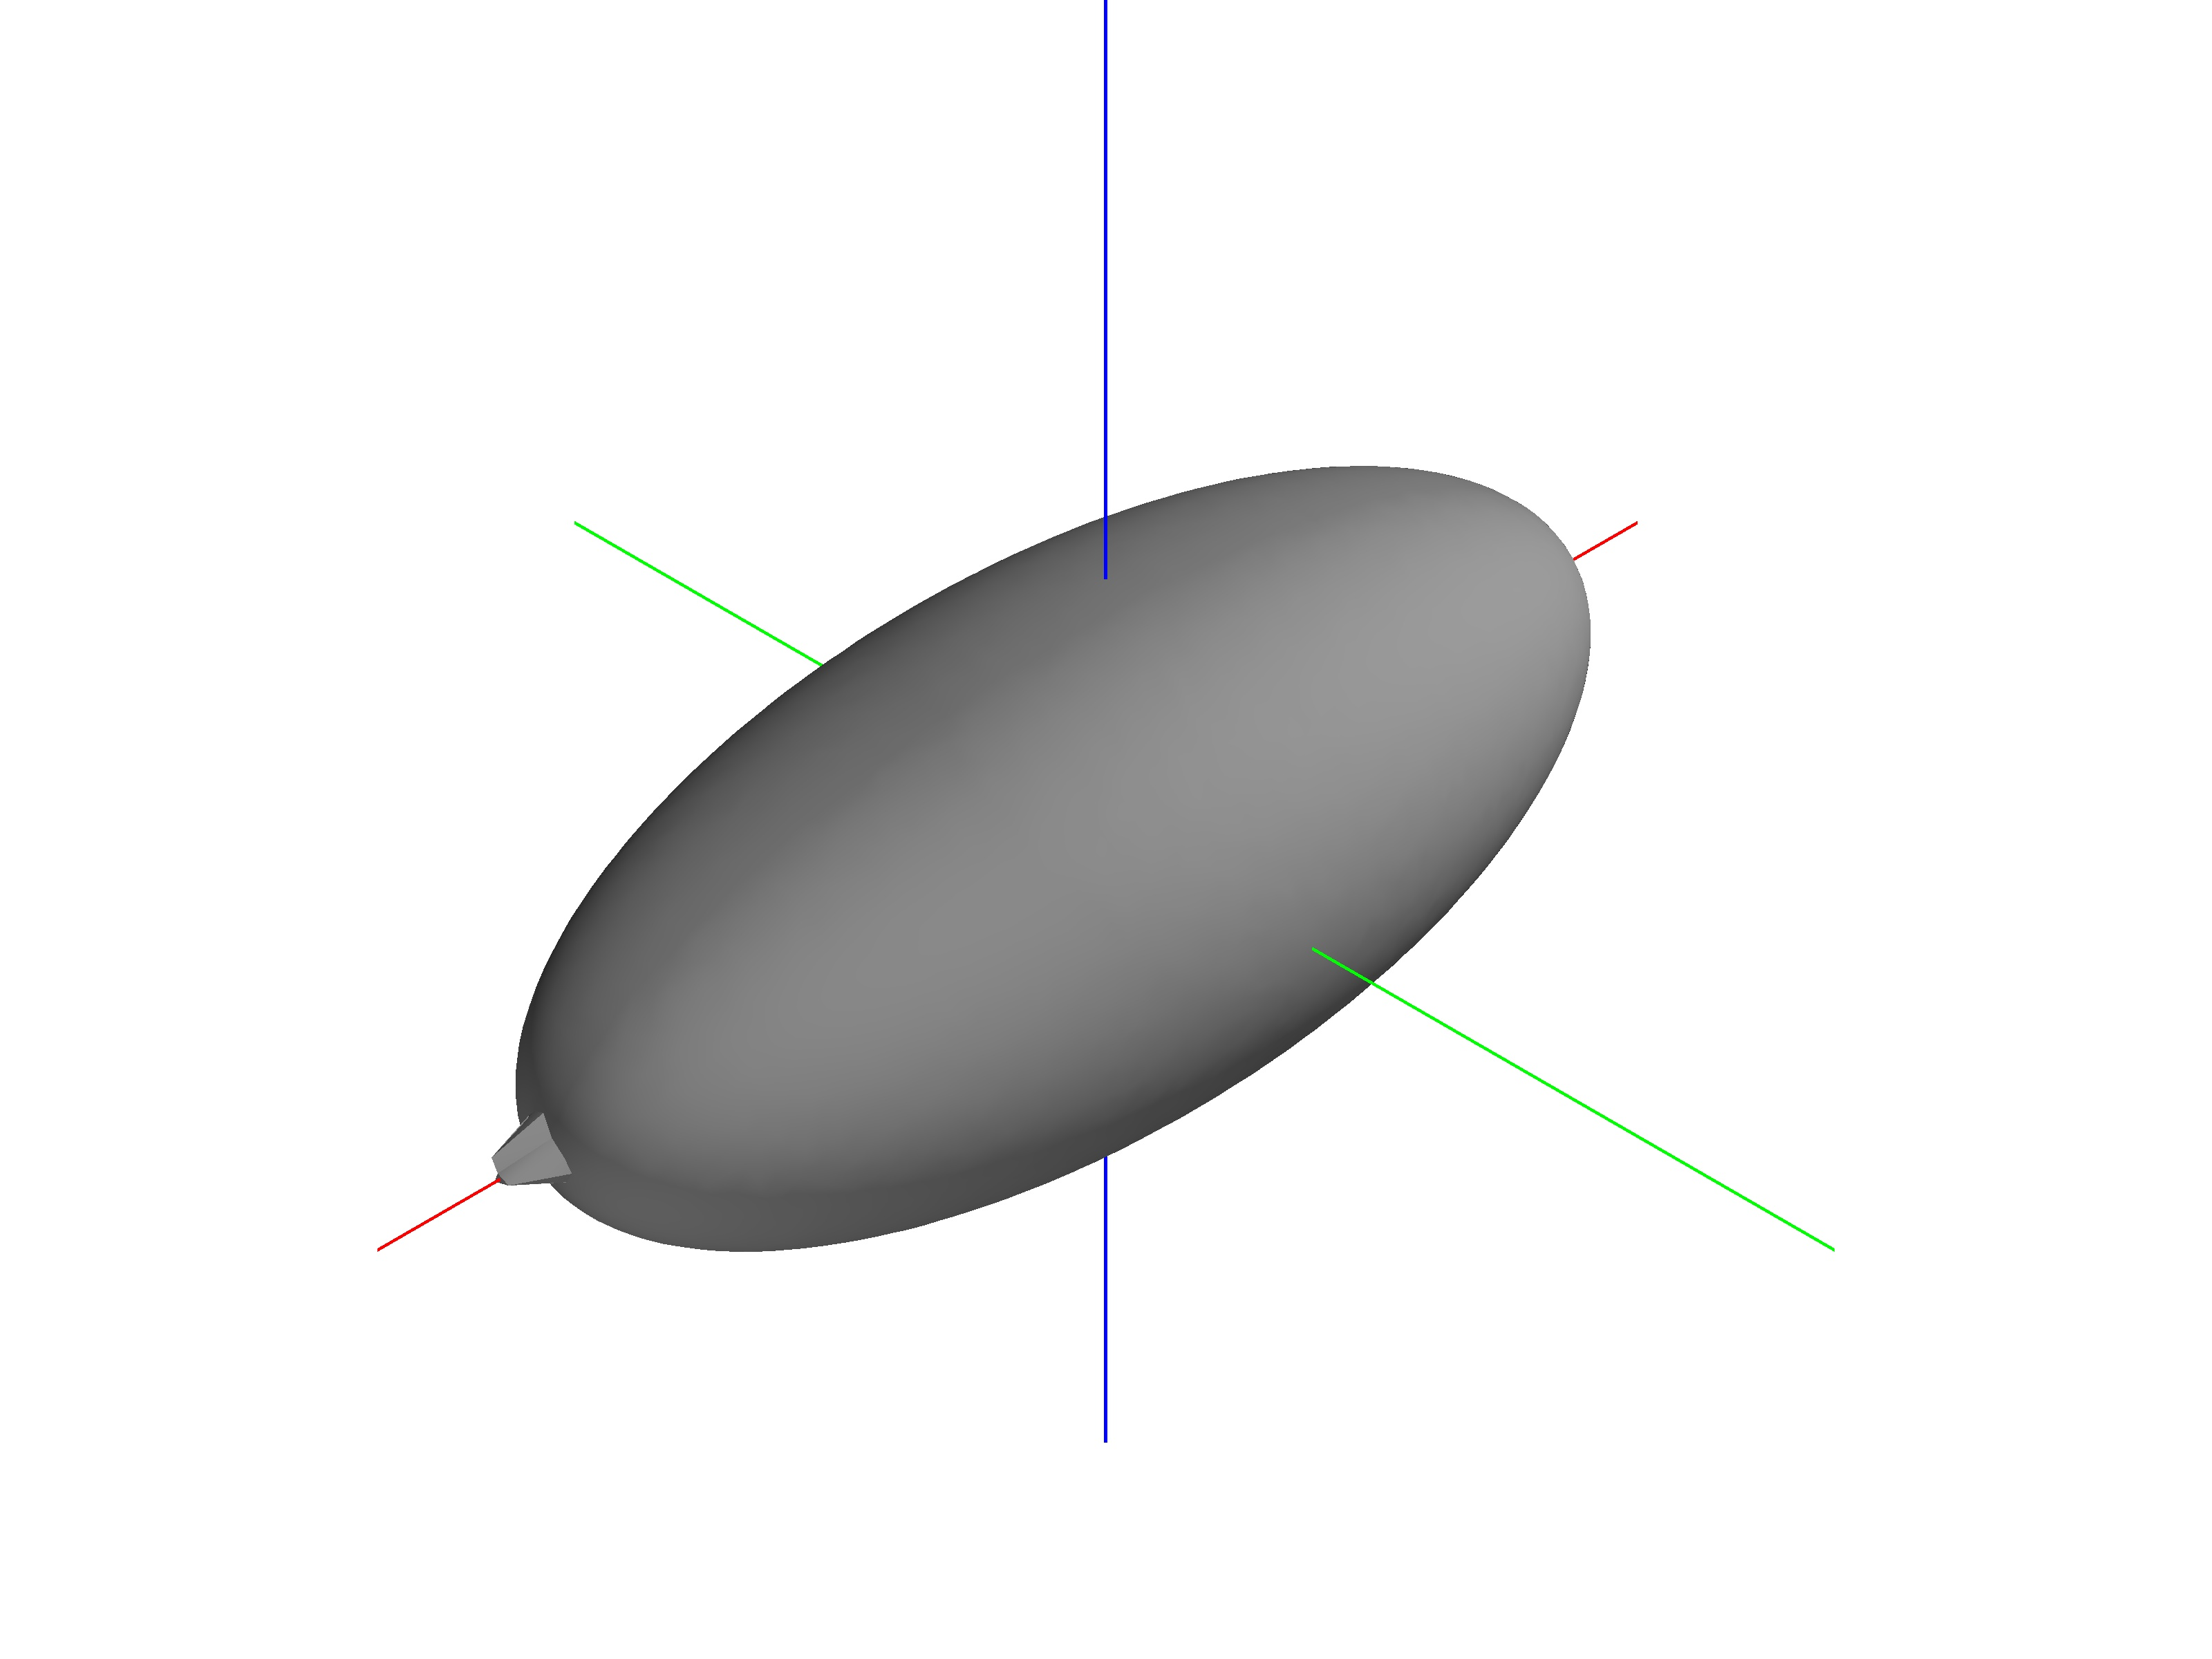
\includegraphics[trim={20cm 15cm 20cm 15cm}, clip,width=0.5\textwidth,keepaspectratio]{figures/mesh_update/geographos/partial_0.jpg}}%
    \subcaptionbox{\SI{25}{\percent} of measurements added\label{fig:geographos_partial_25}}{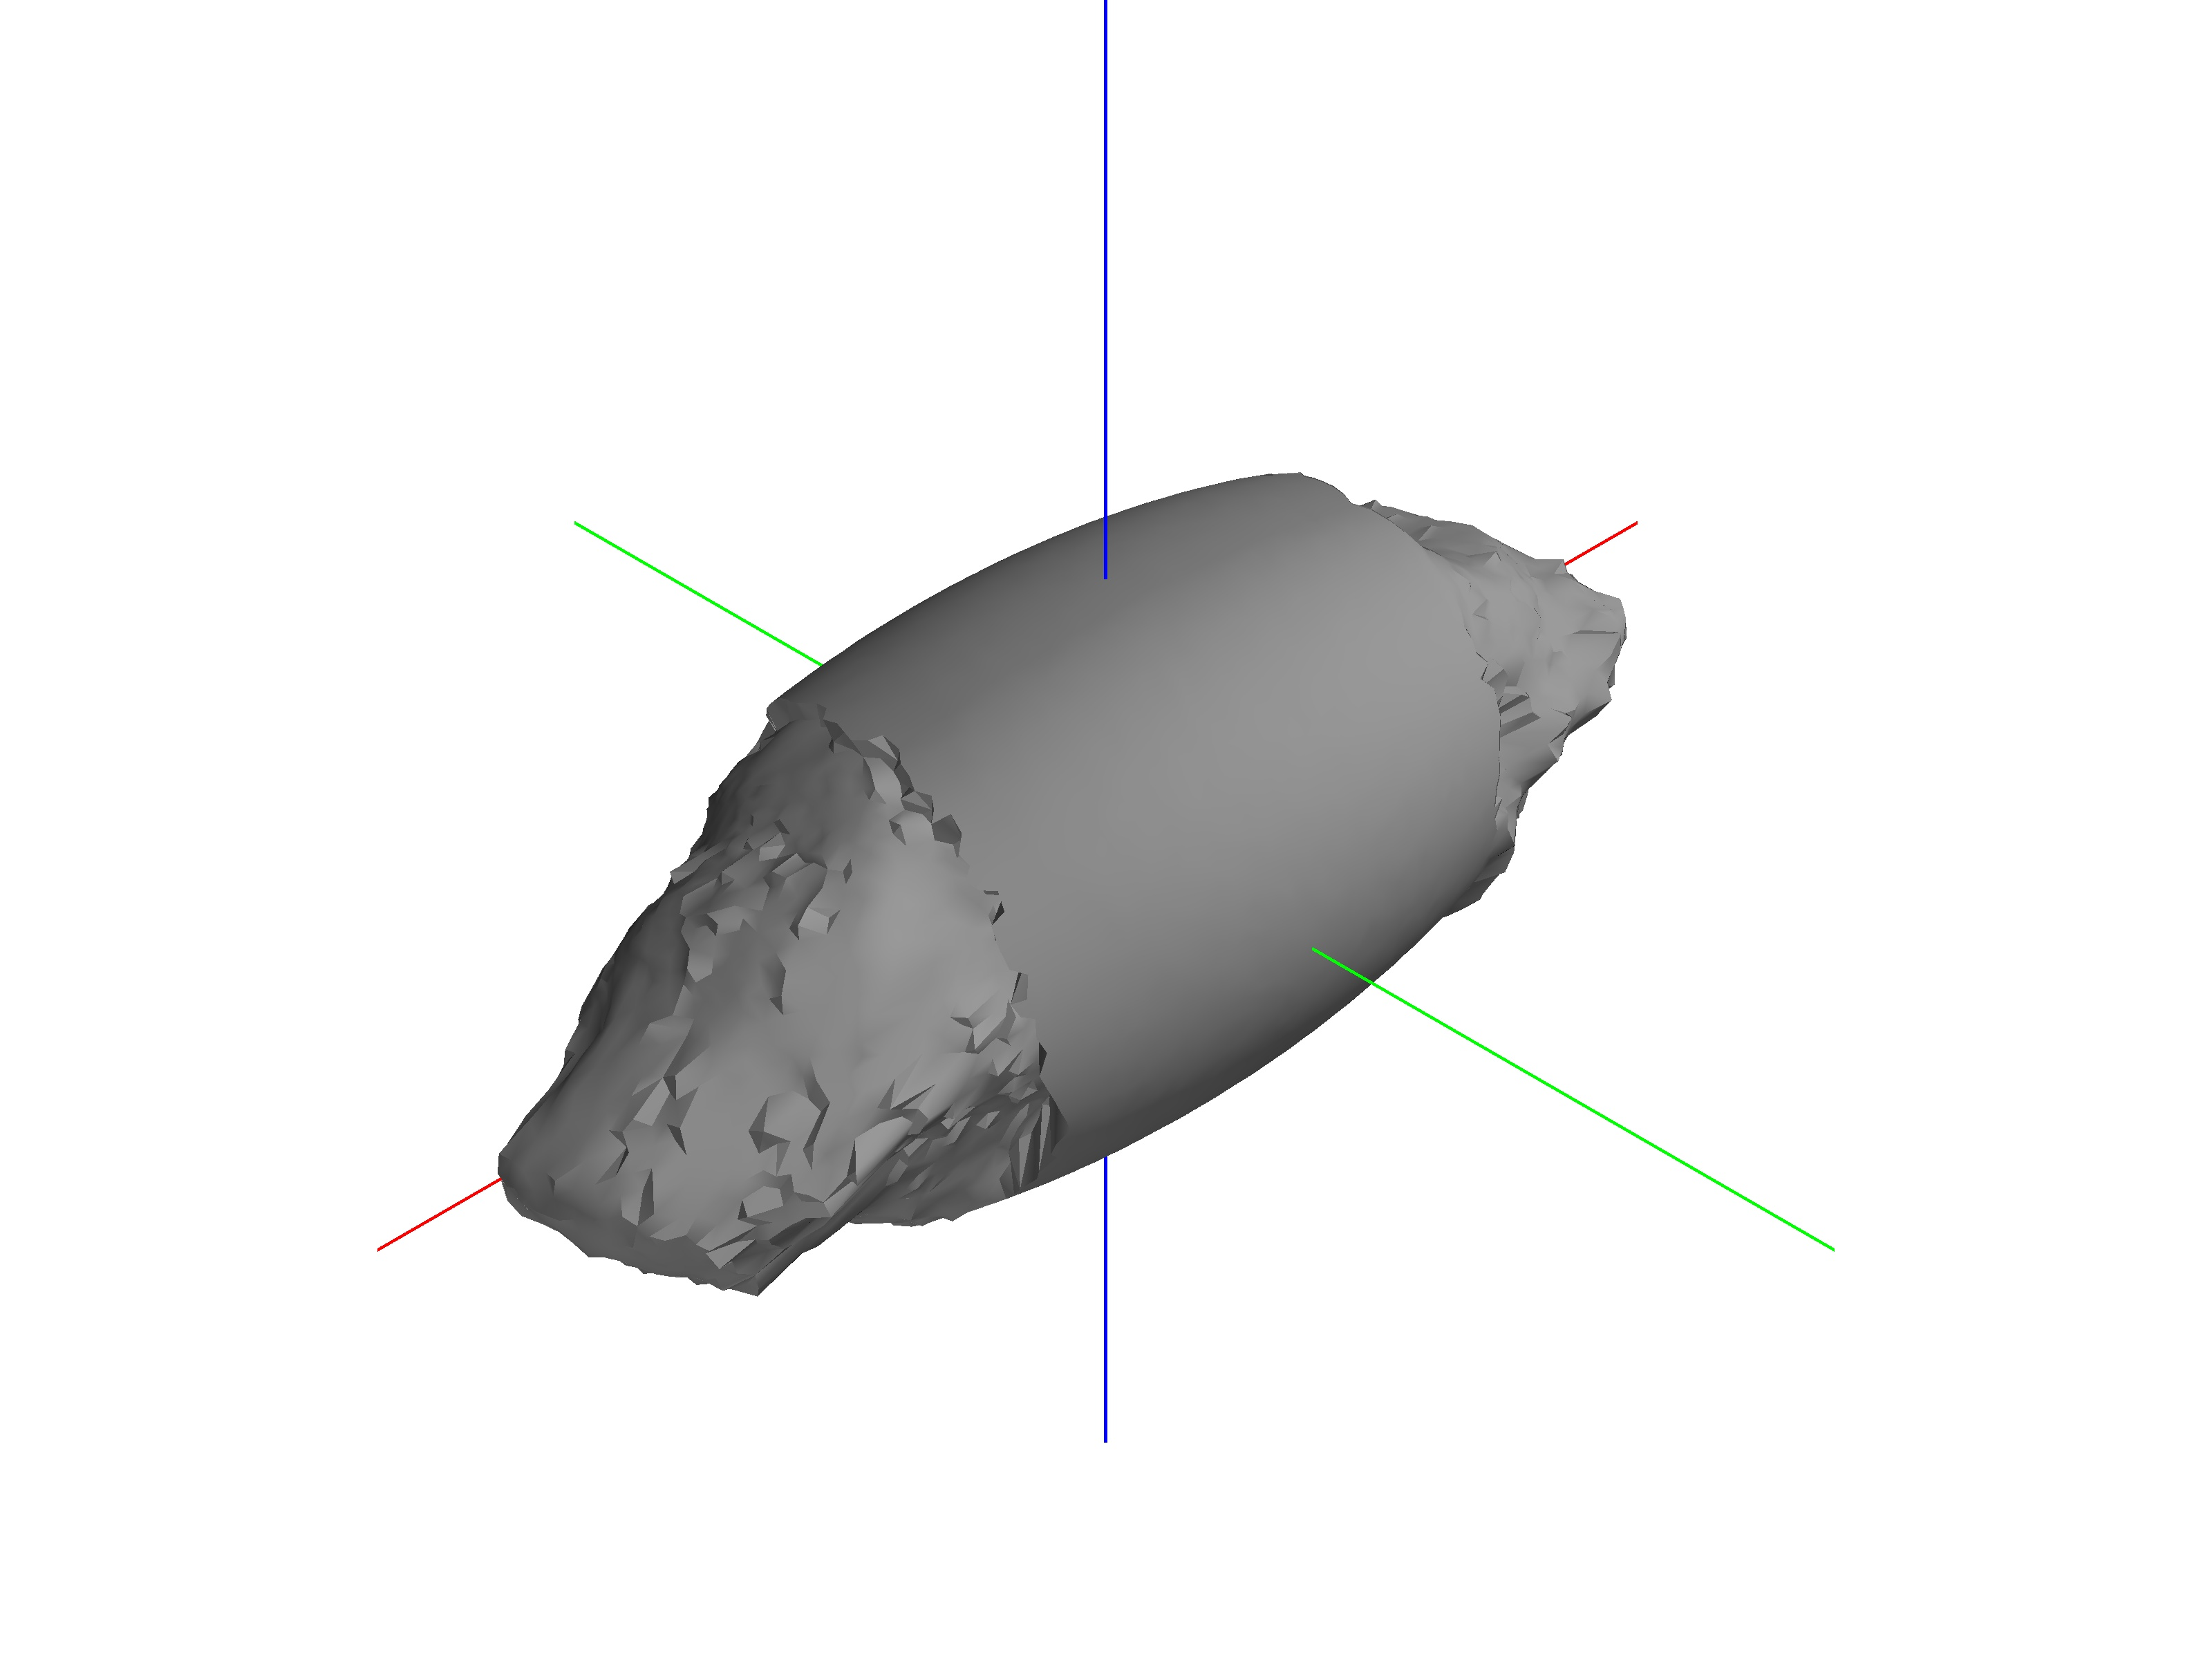
\includegraphics[trim={20cm 15cm 20cm 15cm},clip,keepaspectratio,width=0.5\textwidth]{figures/mesh_update/geographos/partial_1872.jpg}}

    \subcaptionbox{\SI{50}{\percent} of measurements added\label{fig:geographos_partial_50}}{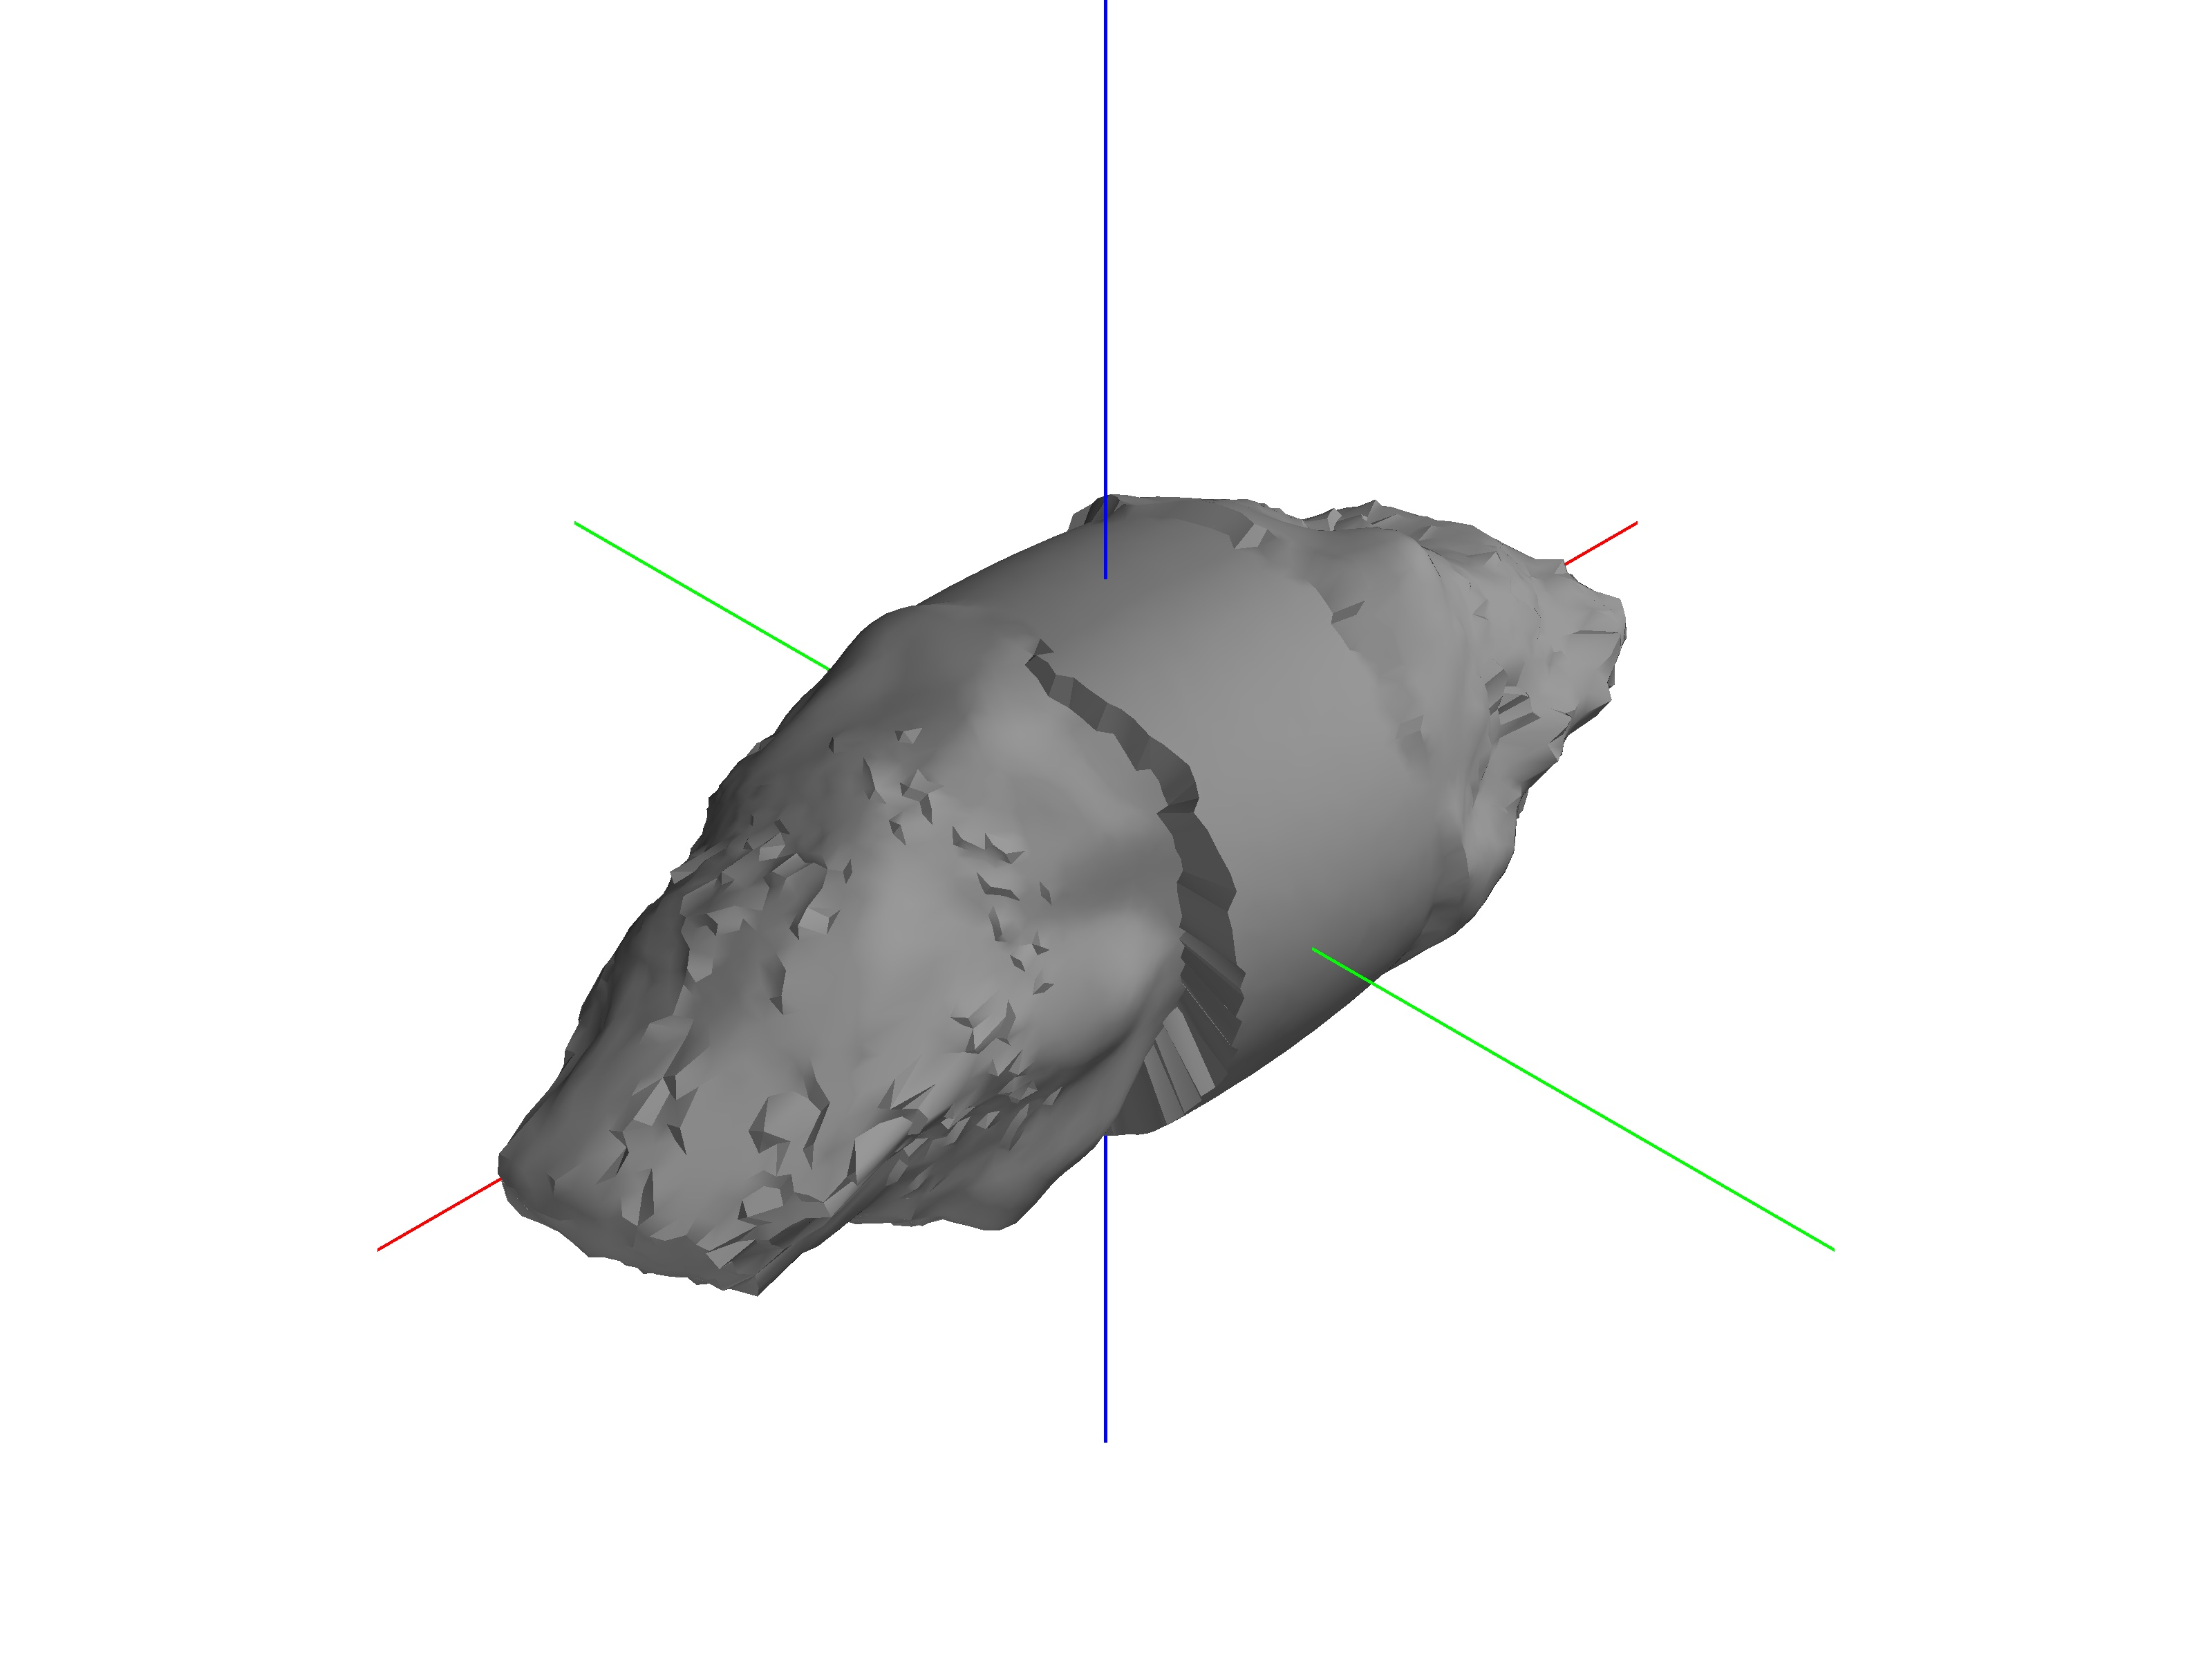
\includegraphics[trim={20cm 15cm 20cm 15cm},clip,keepaspectratio,width=0.5\textwidth]{figures/mesh_update/geographos/partial_3745.jpg}}%
    \subcaptionbox{\SI{75}{\percent} of measurements added\label{fig:geographos_partial_75}}{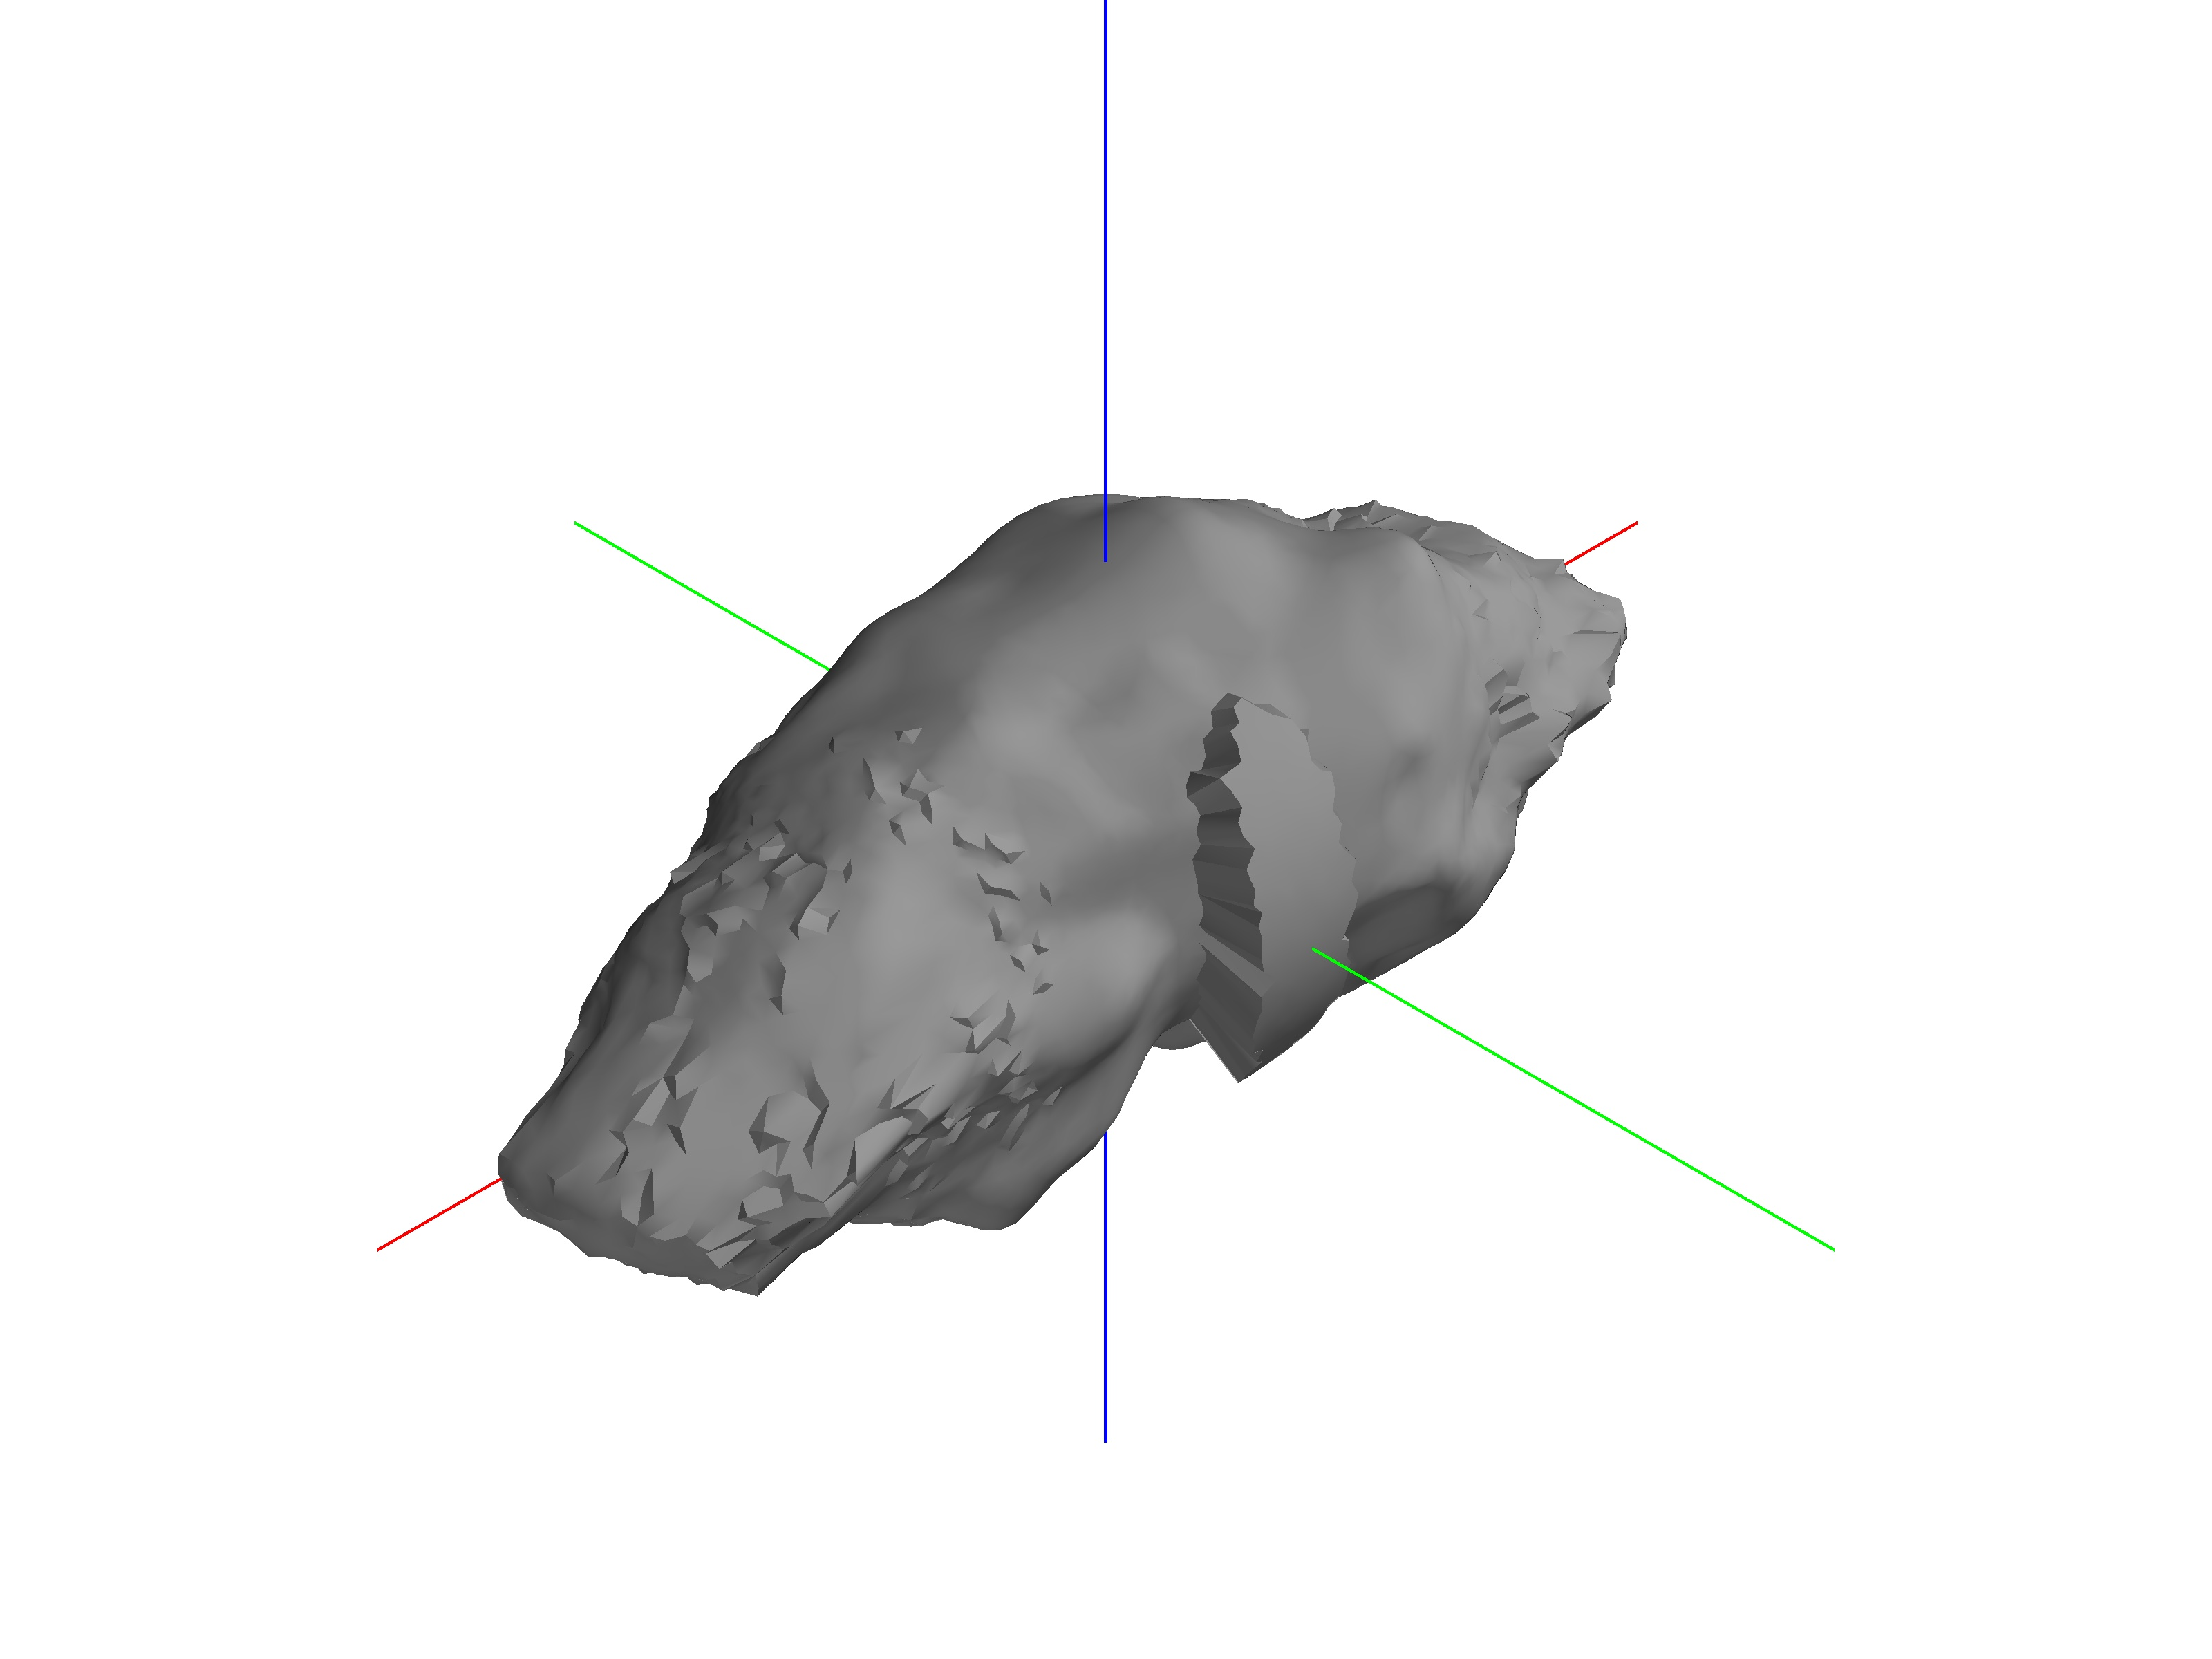
\includegraphics[trim={20cm 15cm 20cm 15cm},clip,keepaspectratio,width=0.5\textwidth]{figures/mesh_update/geographos/partial_5617.jpg}}

    \subcaptionbox{\SI{100}{\percent} of measurements added\label{fig:geographos_partial_100}}{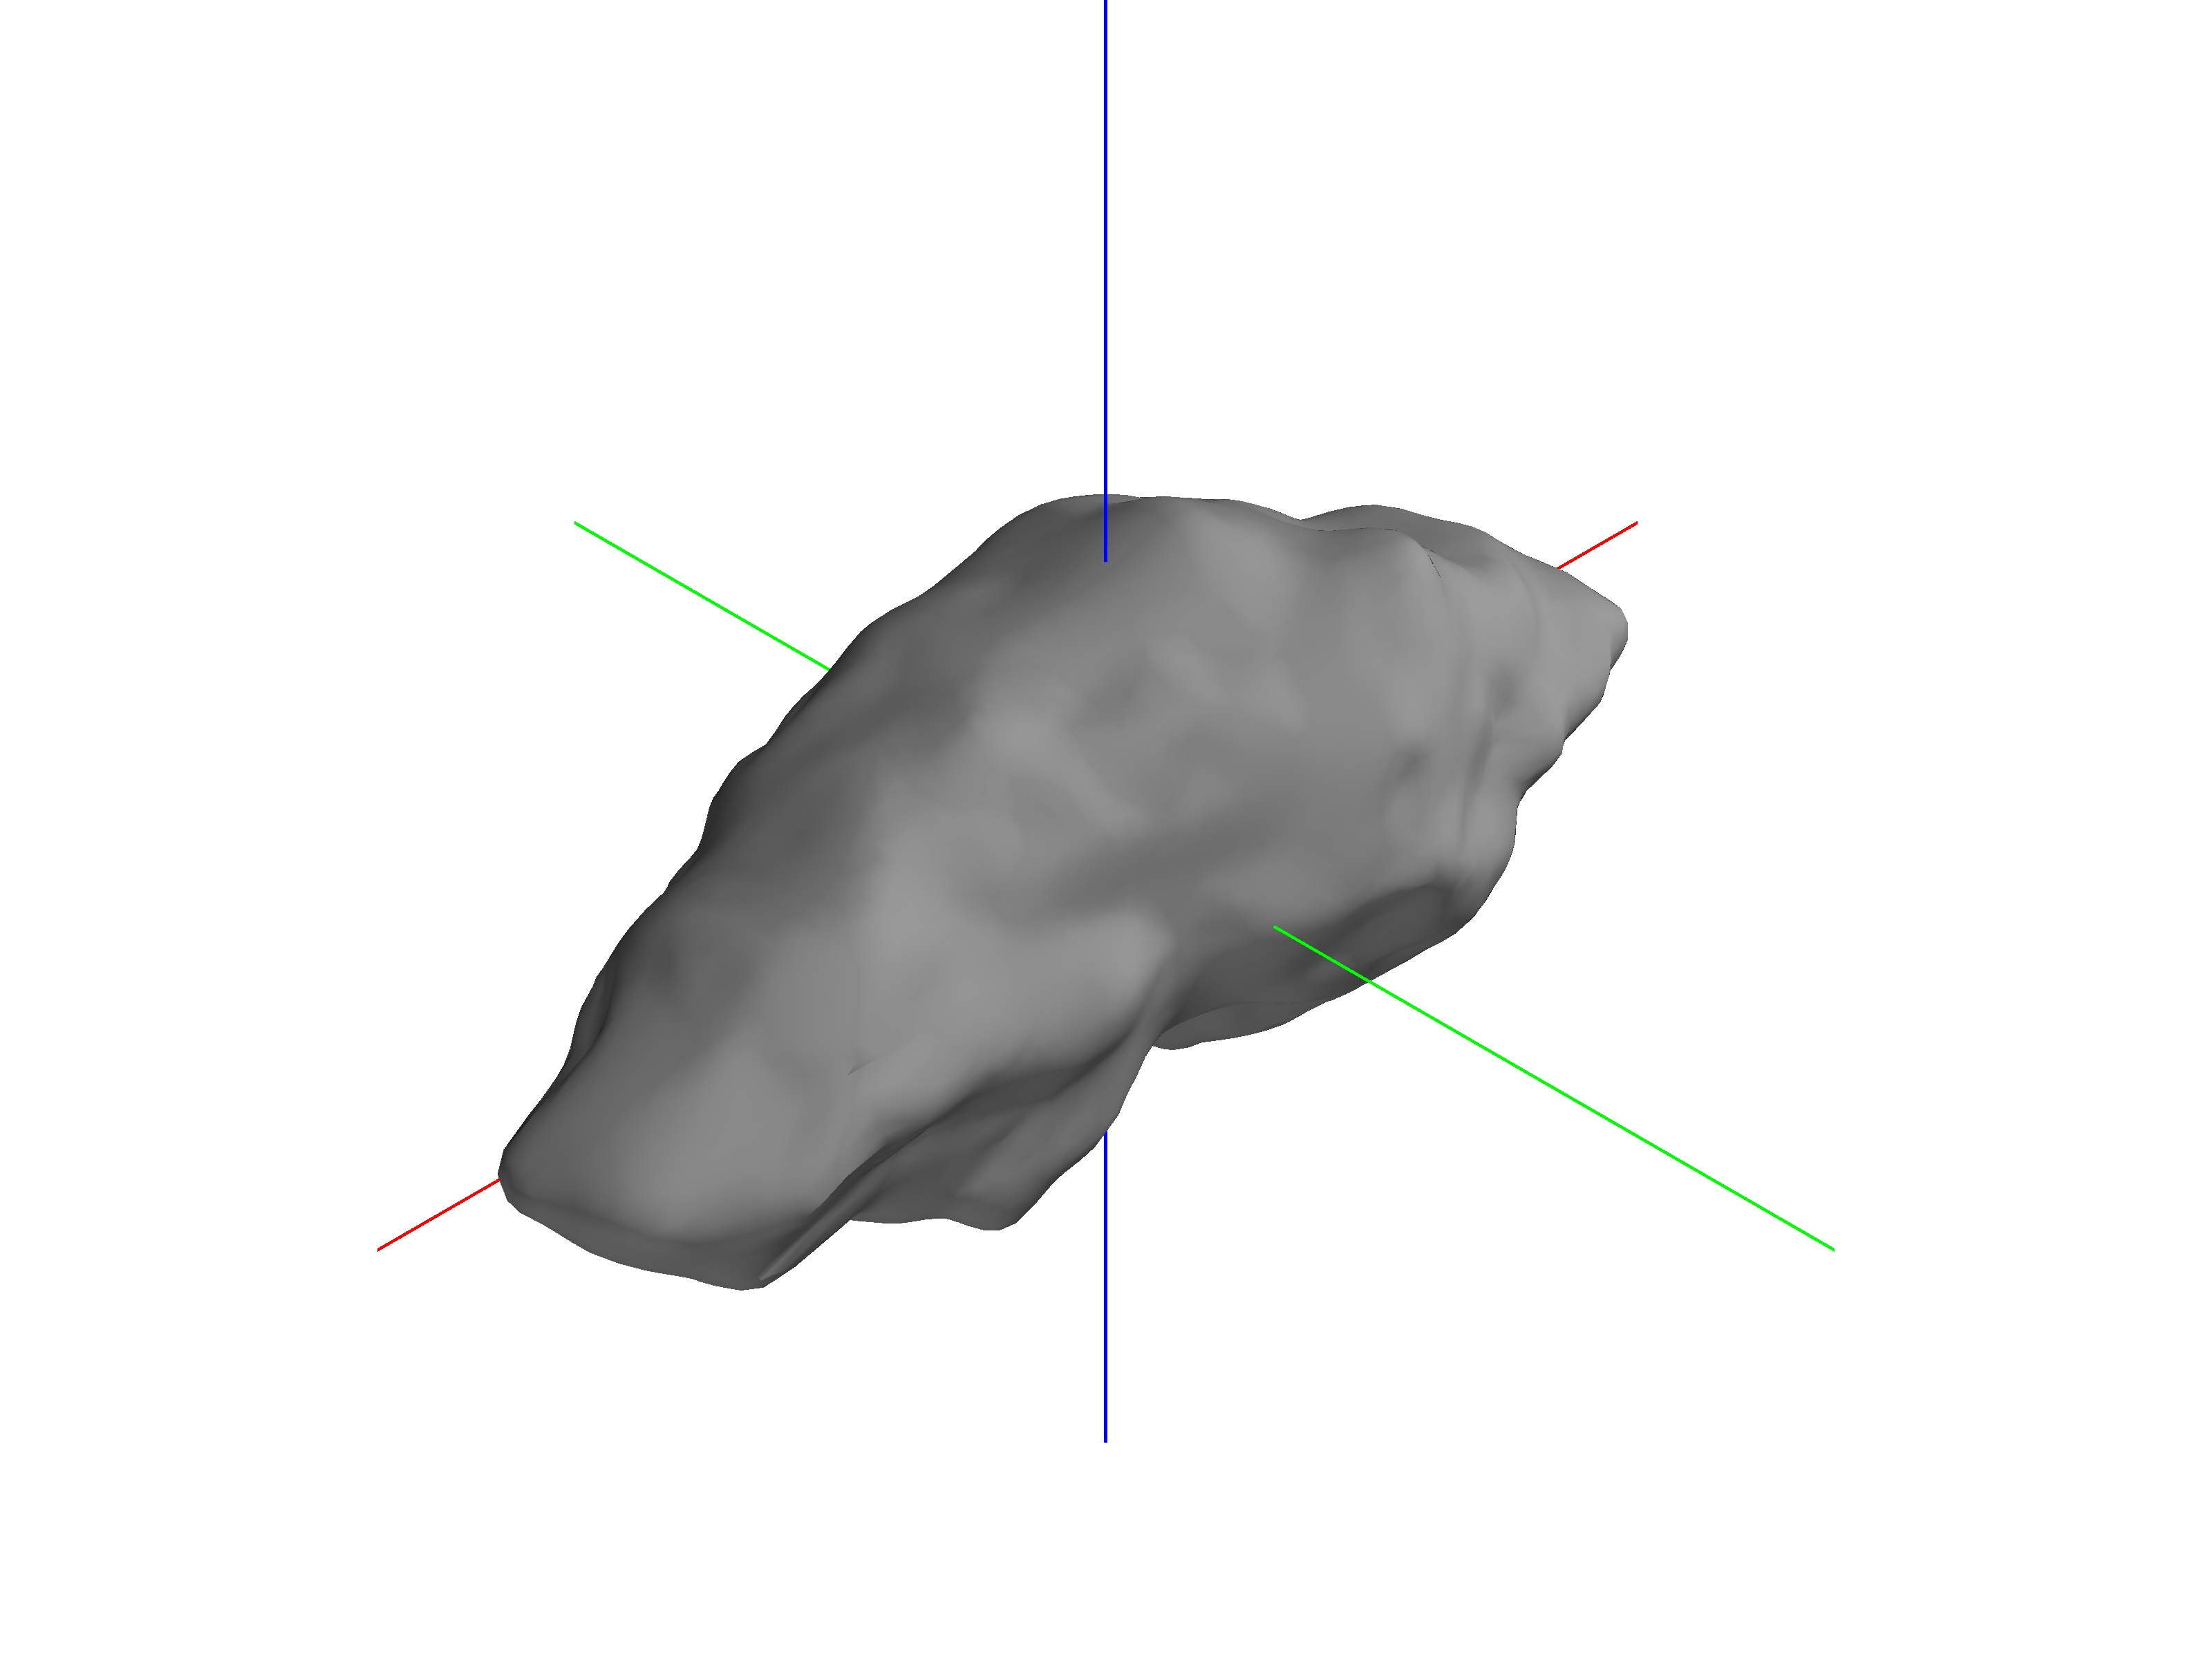
\includegraphics[trim={20cm 15cm 20cm 15cm},clip,keepaspectratio,width=0.5\textwidth]{figures/mesh_update/geographos/partial_7489.jpg}}%
    \subcaptionbox{True Shape Model\label{fig:geographos_truth}}{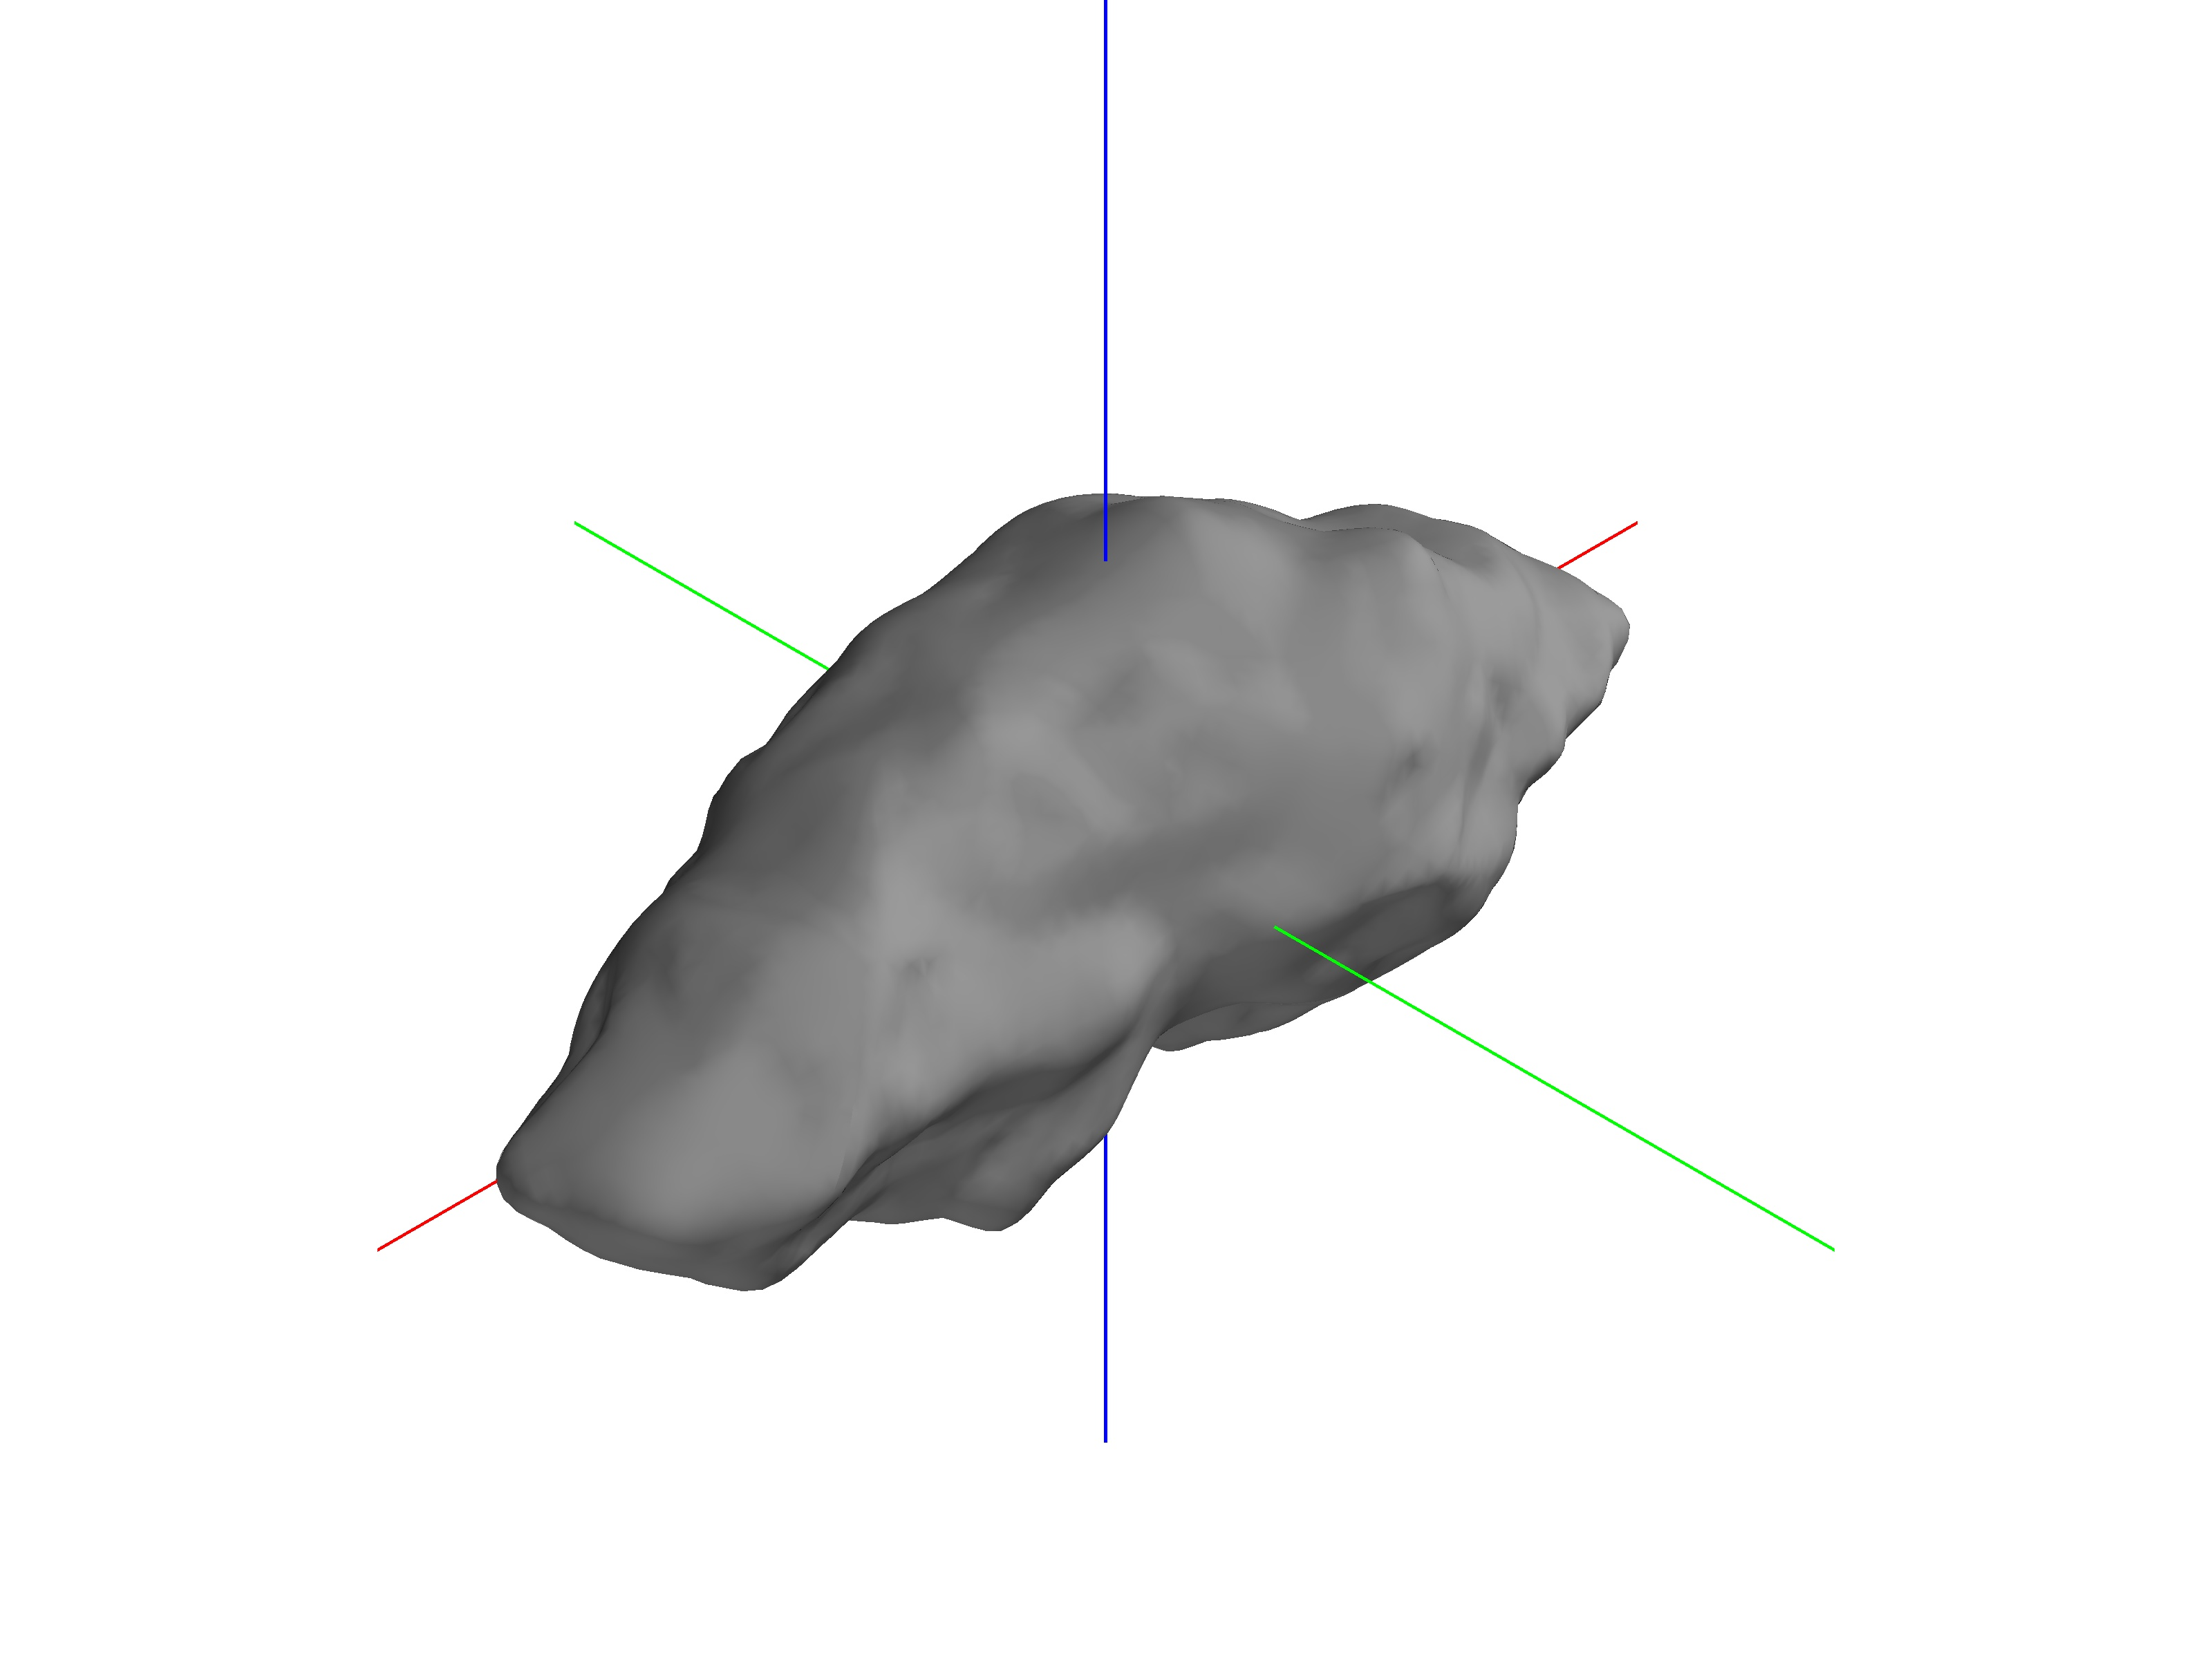
\includegraphics[trim={20cm 15cm 20cm 15cm},clip,keepaspectratio,width=0.5\textwidth]{figures/mesh_update/geographos/truth.jpg}}
    \caption[Asteroid Geographos incremental reconstruction]{Incremental reconstruction of asteroid Geographos~\label{fig:geographos_reconstruction}}
\end{figure}

\num{1620} Geographos is a highly elongated stony asteroid of the Apollo group.
Discovered in \num{1951}, Geographos is a potentially hazardous asteroid which passes sufficiently close to the Earth to present a hazard.
\Cref{fig:geographos_reconstruction} shows the shape reconstruction for asteroid Geographos at several distinct points during the process.
Comparing~\cref{fig:geographos_partial_100,fig:geographos_truth} shows that the final shape closely matches the true radar model.
In~\cref{fig:geographos_metrics} we display the vertex uncertainty and mesh volume as a function of time.
The plots show that the reconstruction achieves an accurate shape estimate with a total volume which closely matches the true volume.

\begin{figure}[htbp]
    \centering
    \tikzsetnextfilename{geographos_metrics}
\begin{tikzpicture}[baseline]
    \begin{groupplot}[
        group style={
            group name={geographos_metrics},
            group size=1 by 2,
            xlabels at=edge bottom,
            ylabels at=edge left,
            xticklabels at=edge bottom,
        },
        xlabel={Normalized Time},
        scale only axis,
        width=0.8\textwidth,
        height=0.1\textheight,
        ylabel style={align=center},
    ]
    \nextgroupplot[ylabel={Normalized\\Uncertainty}]
    \addplot [ultra thick, color=blue, mark=none] table [x=NORMALIZED_TIME, y=NORMALIZED_UNCERTAINTY, col sep=comma] {figures/mesh_update/geographos/uncertainty.csv};
    \addplot [ultra thick,red, mark=none, dashed] coordinates {
        (0.0, 0.0) (1.0, 0.0) 
    };

    \nextgroupplot[ylabel={Volume Percent\\Error}]
    \addplot [ultra thick, blue, mark=none] table [x=NORMALIZED_TIME, y=VOLUME_PERCENT_ERROR, col sep=comma] {figures/mesh_update/geographos/volume.csv};
        \addplot [ultra thick,red, mark=none, dashed] coordinates {
            (0.0, 0.0) (1.0, 0.0) 
        };
\end{groupplot}
\end{tikzpicture}


    \caption{Normalized uncertainty and volume percent error for Geographos\label{fig:geographos_metrics}}
\end{figure}

\num{6489} Golevka is a small angular shaped asteroid of the Apollo group.
Discovered in \num{1995}, Golevka is a potentially hazardous asteroid which passes sufficiently close to the Earth to present a hazard.
\Cref{fig:golevka_reconstruction} shows the shape reconstruction for asteroid Golevka at several distinct points during the process.
\begin{figure}[htbp]
    \centering
    \subcaptionbox{Initial Shape Estimate\label{fig:golevka_partial_0}}{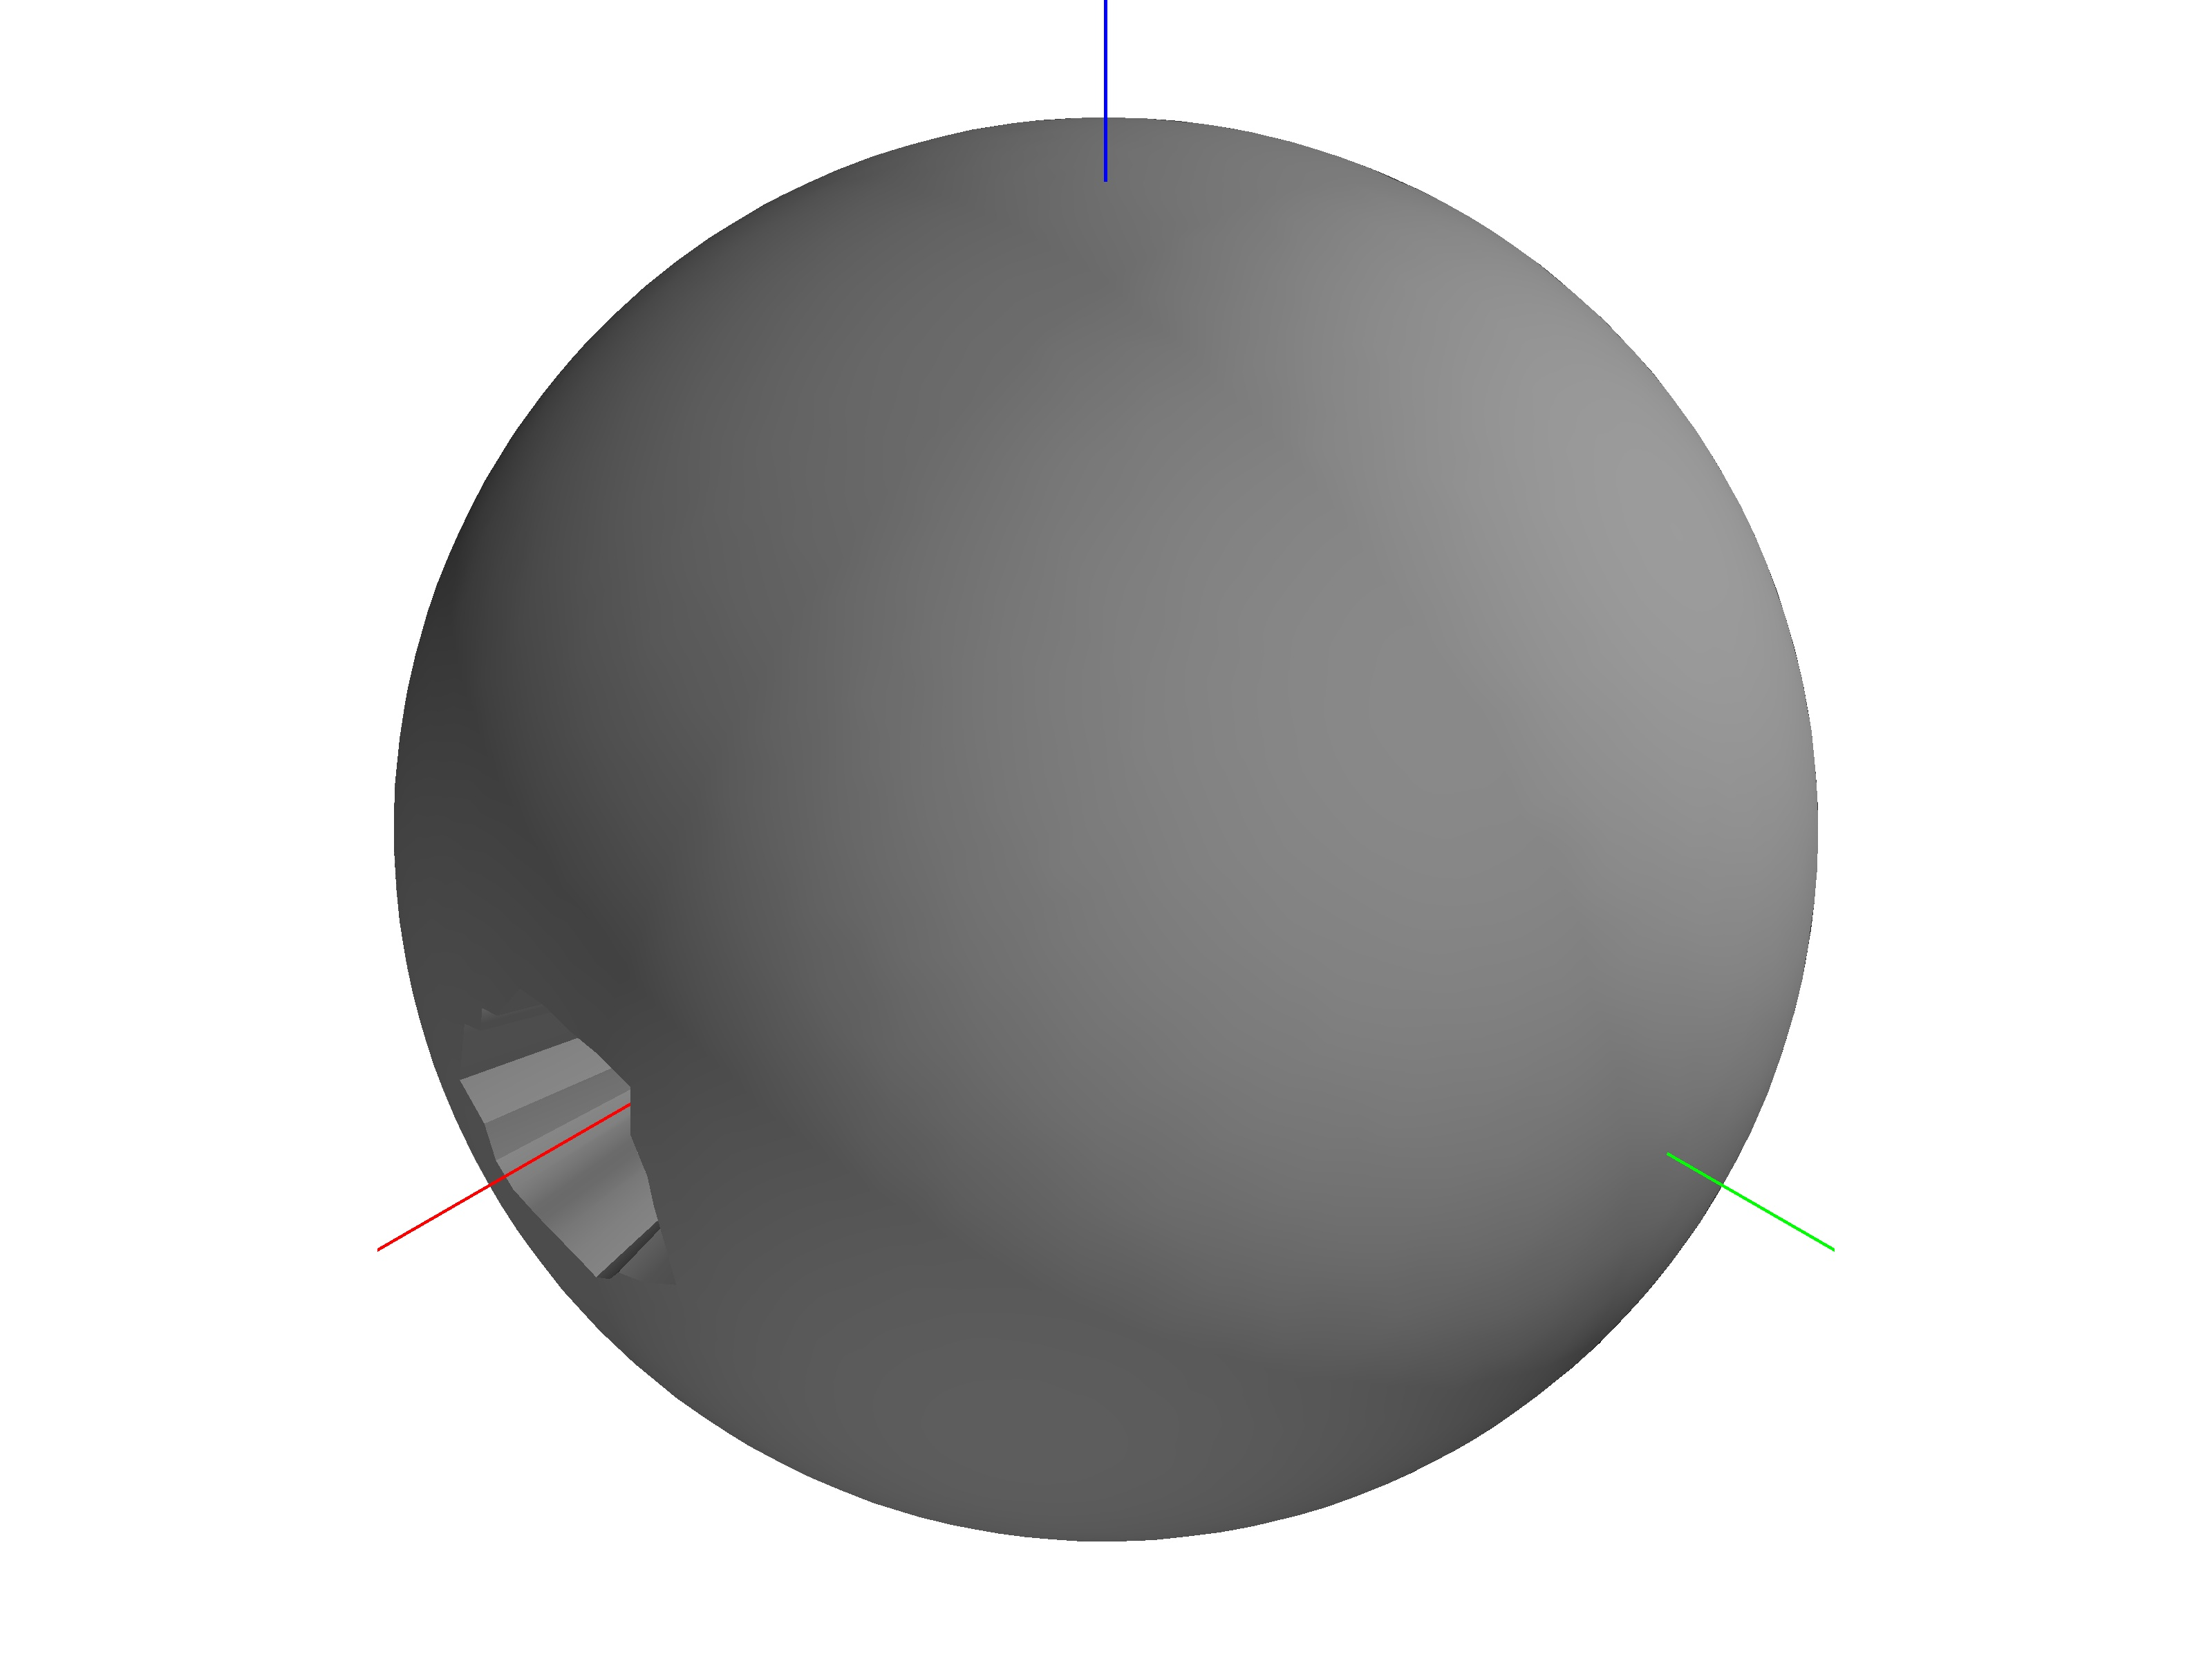
\includegraphics[trim={20cm 5cm 20cm 5cm},clip,keepaspectratio,width=0.5\textwidth,height=0.25\textheight]{figures/mesh_update/golevka/partial_0.jpg}}%
    \subcaptionbox{\SI{25}{\percent} of measurements added\label{fig:golevka_partial_25}}{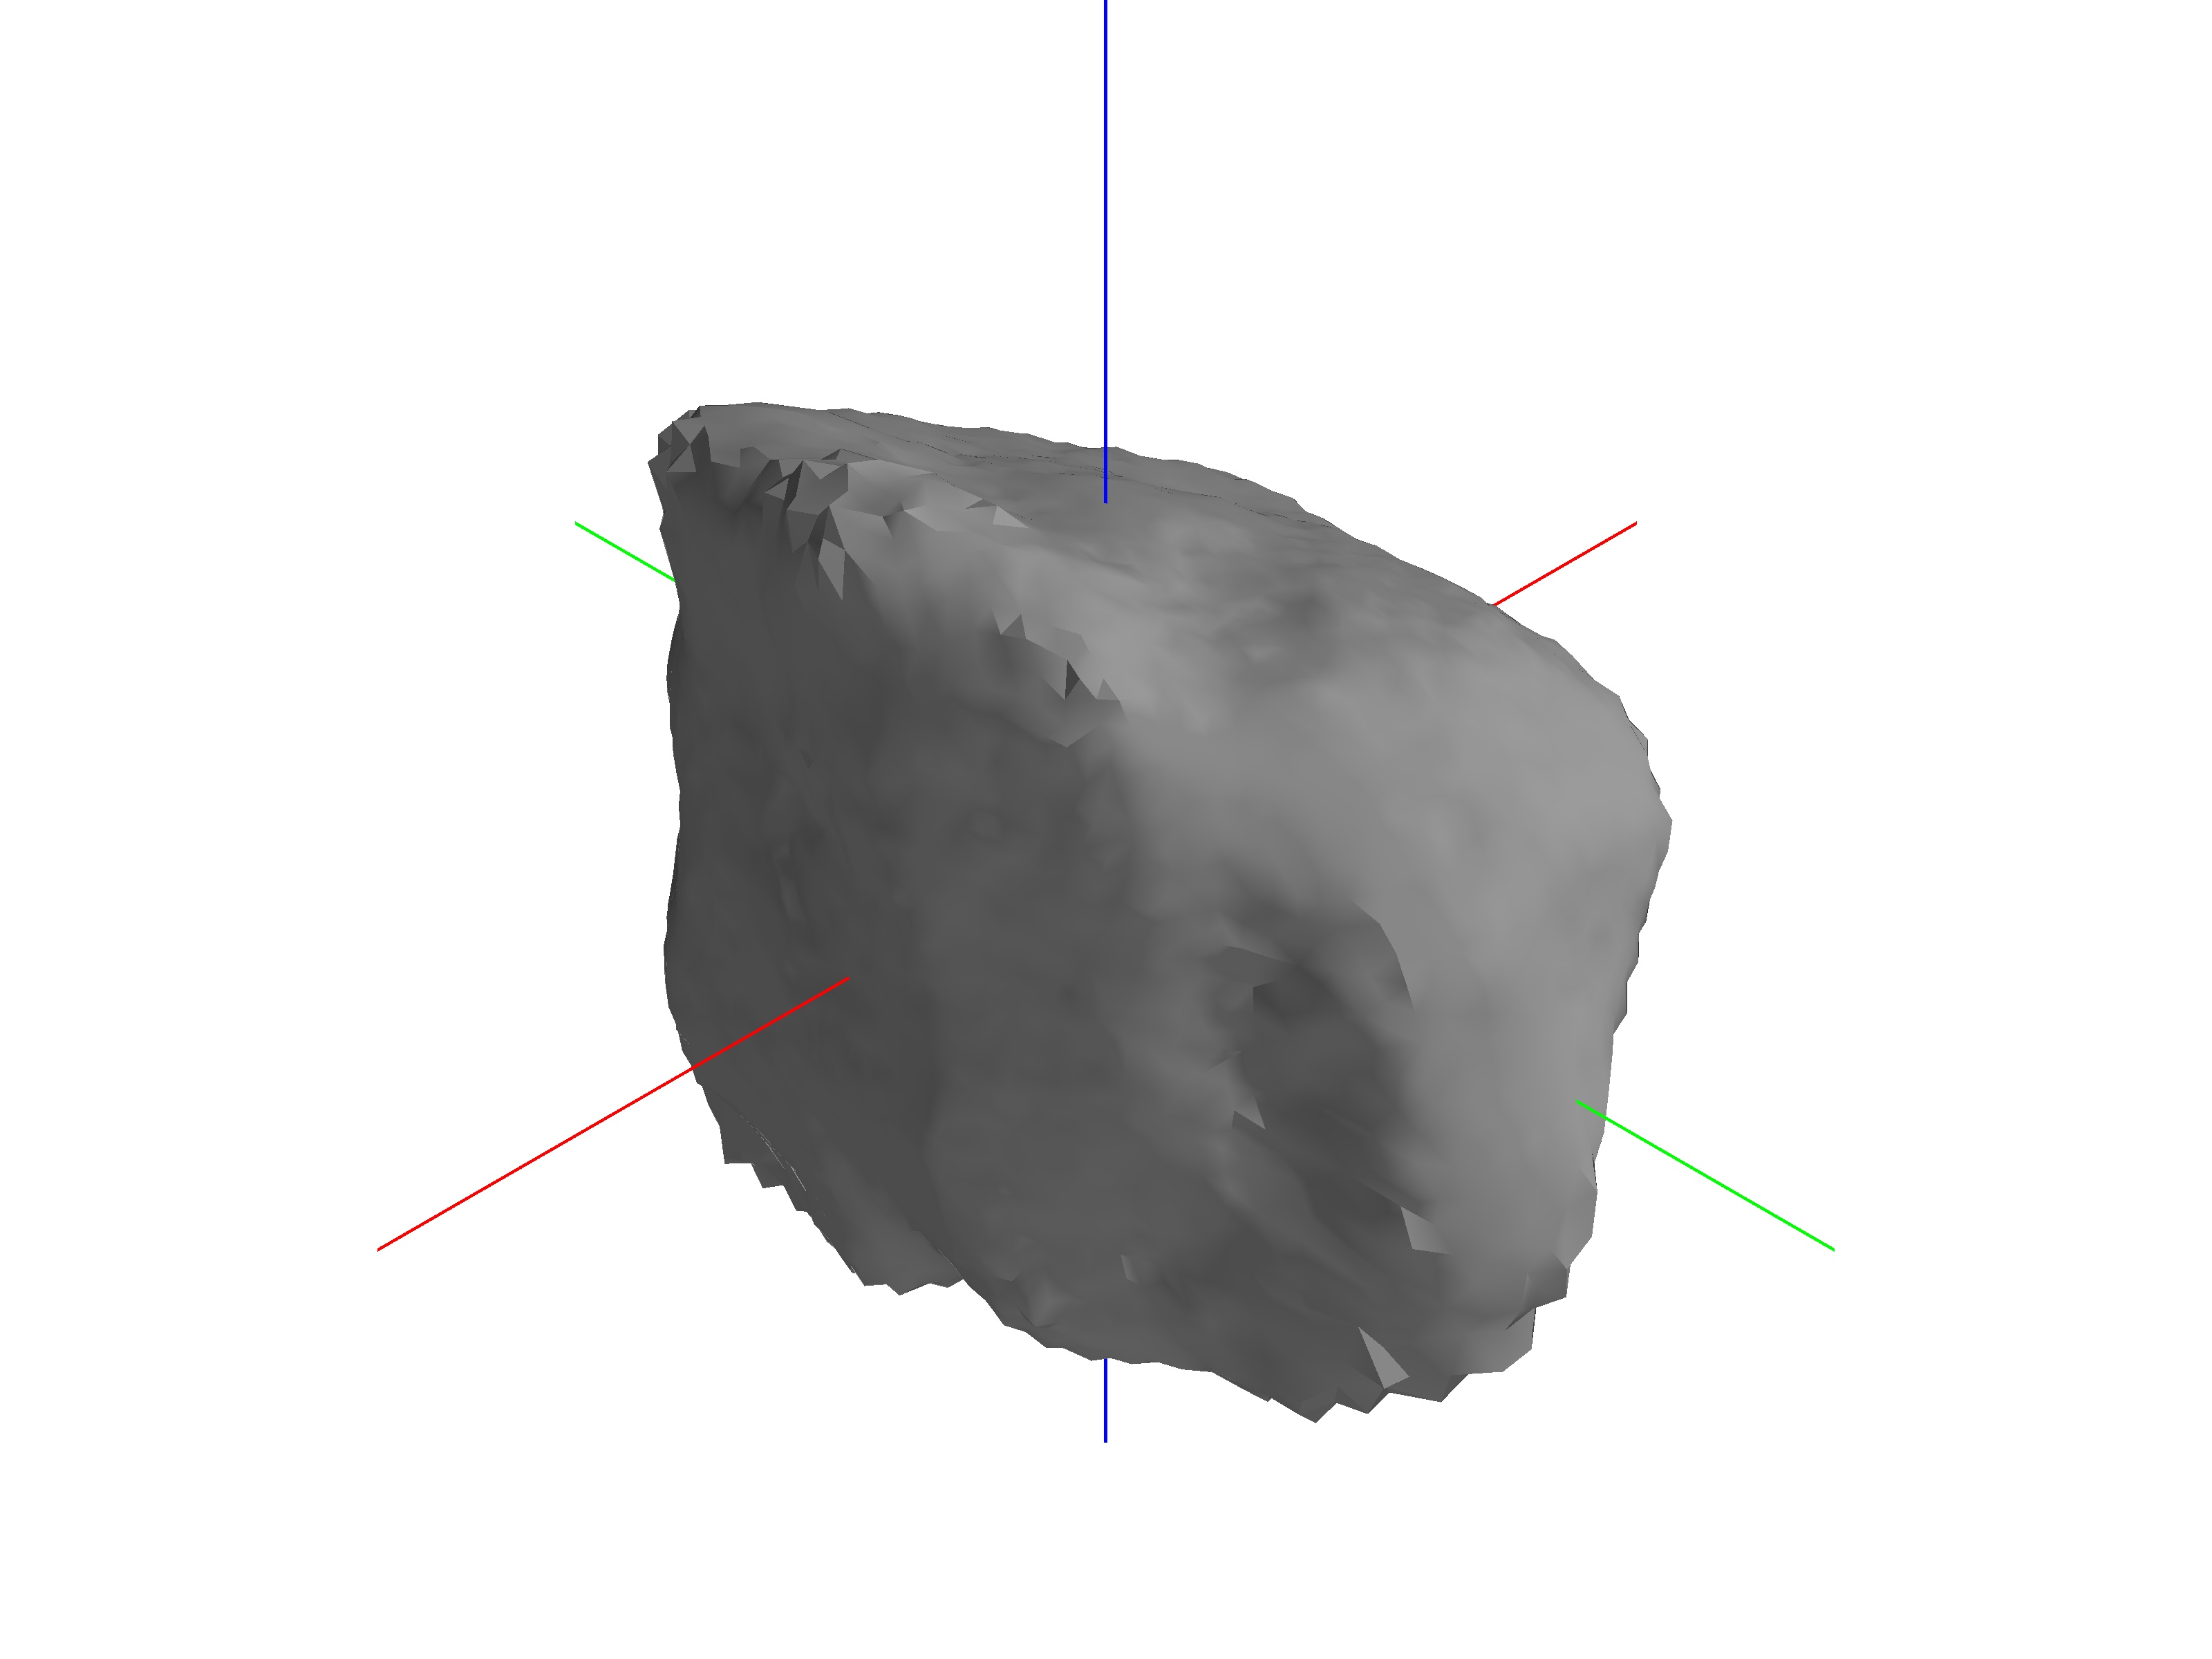
\includegraphics[trim={20cm 10cm 20cm 10cm},clip,keepaspectratio,width=0.5\textwidth,height=0.25\textheight]{figures/mesh_update/golevka/partial_1321.jpg}}\\%

    \subcaptionbox{\SI{50}{\percent} of measurements added\label{fig:golevka_partial_50}}{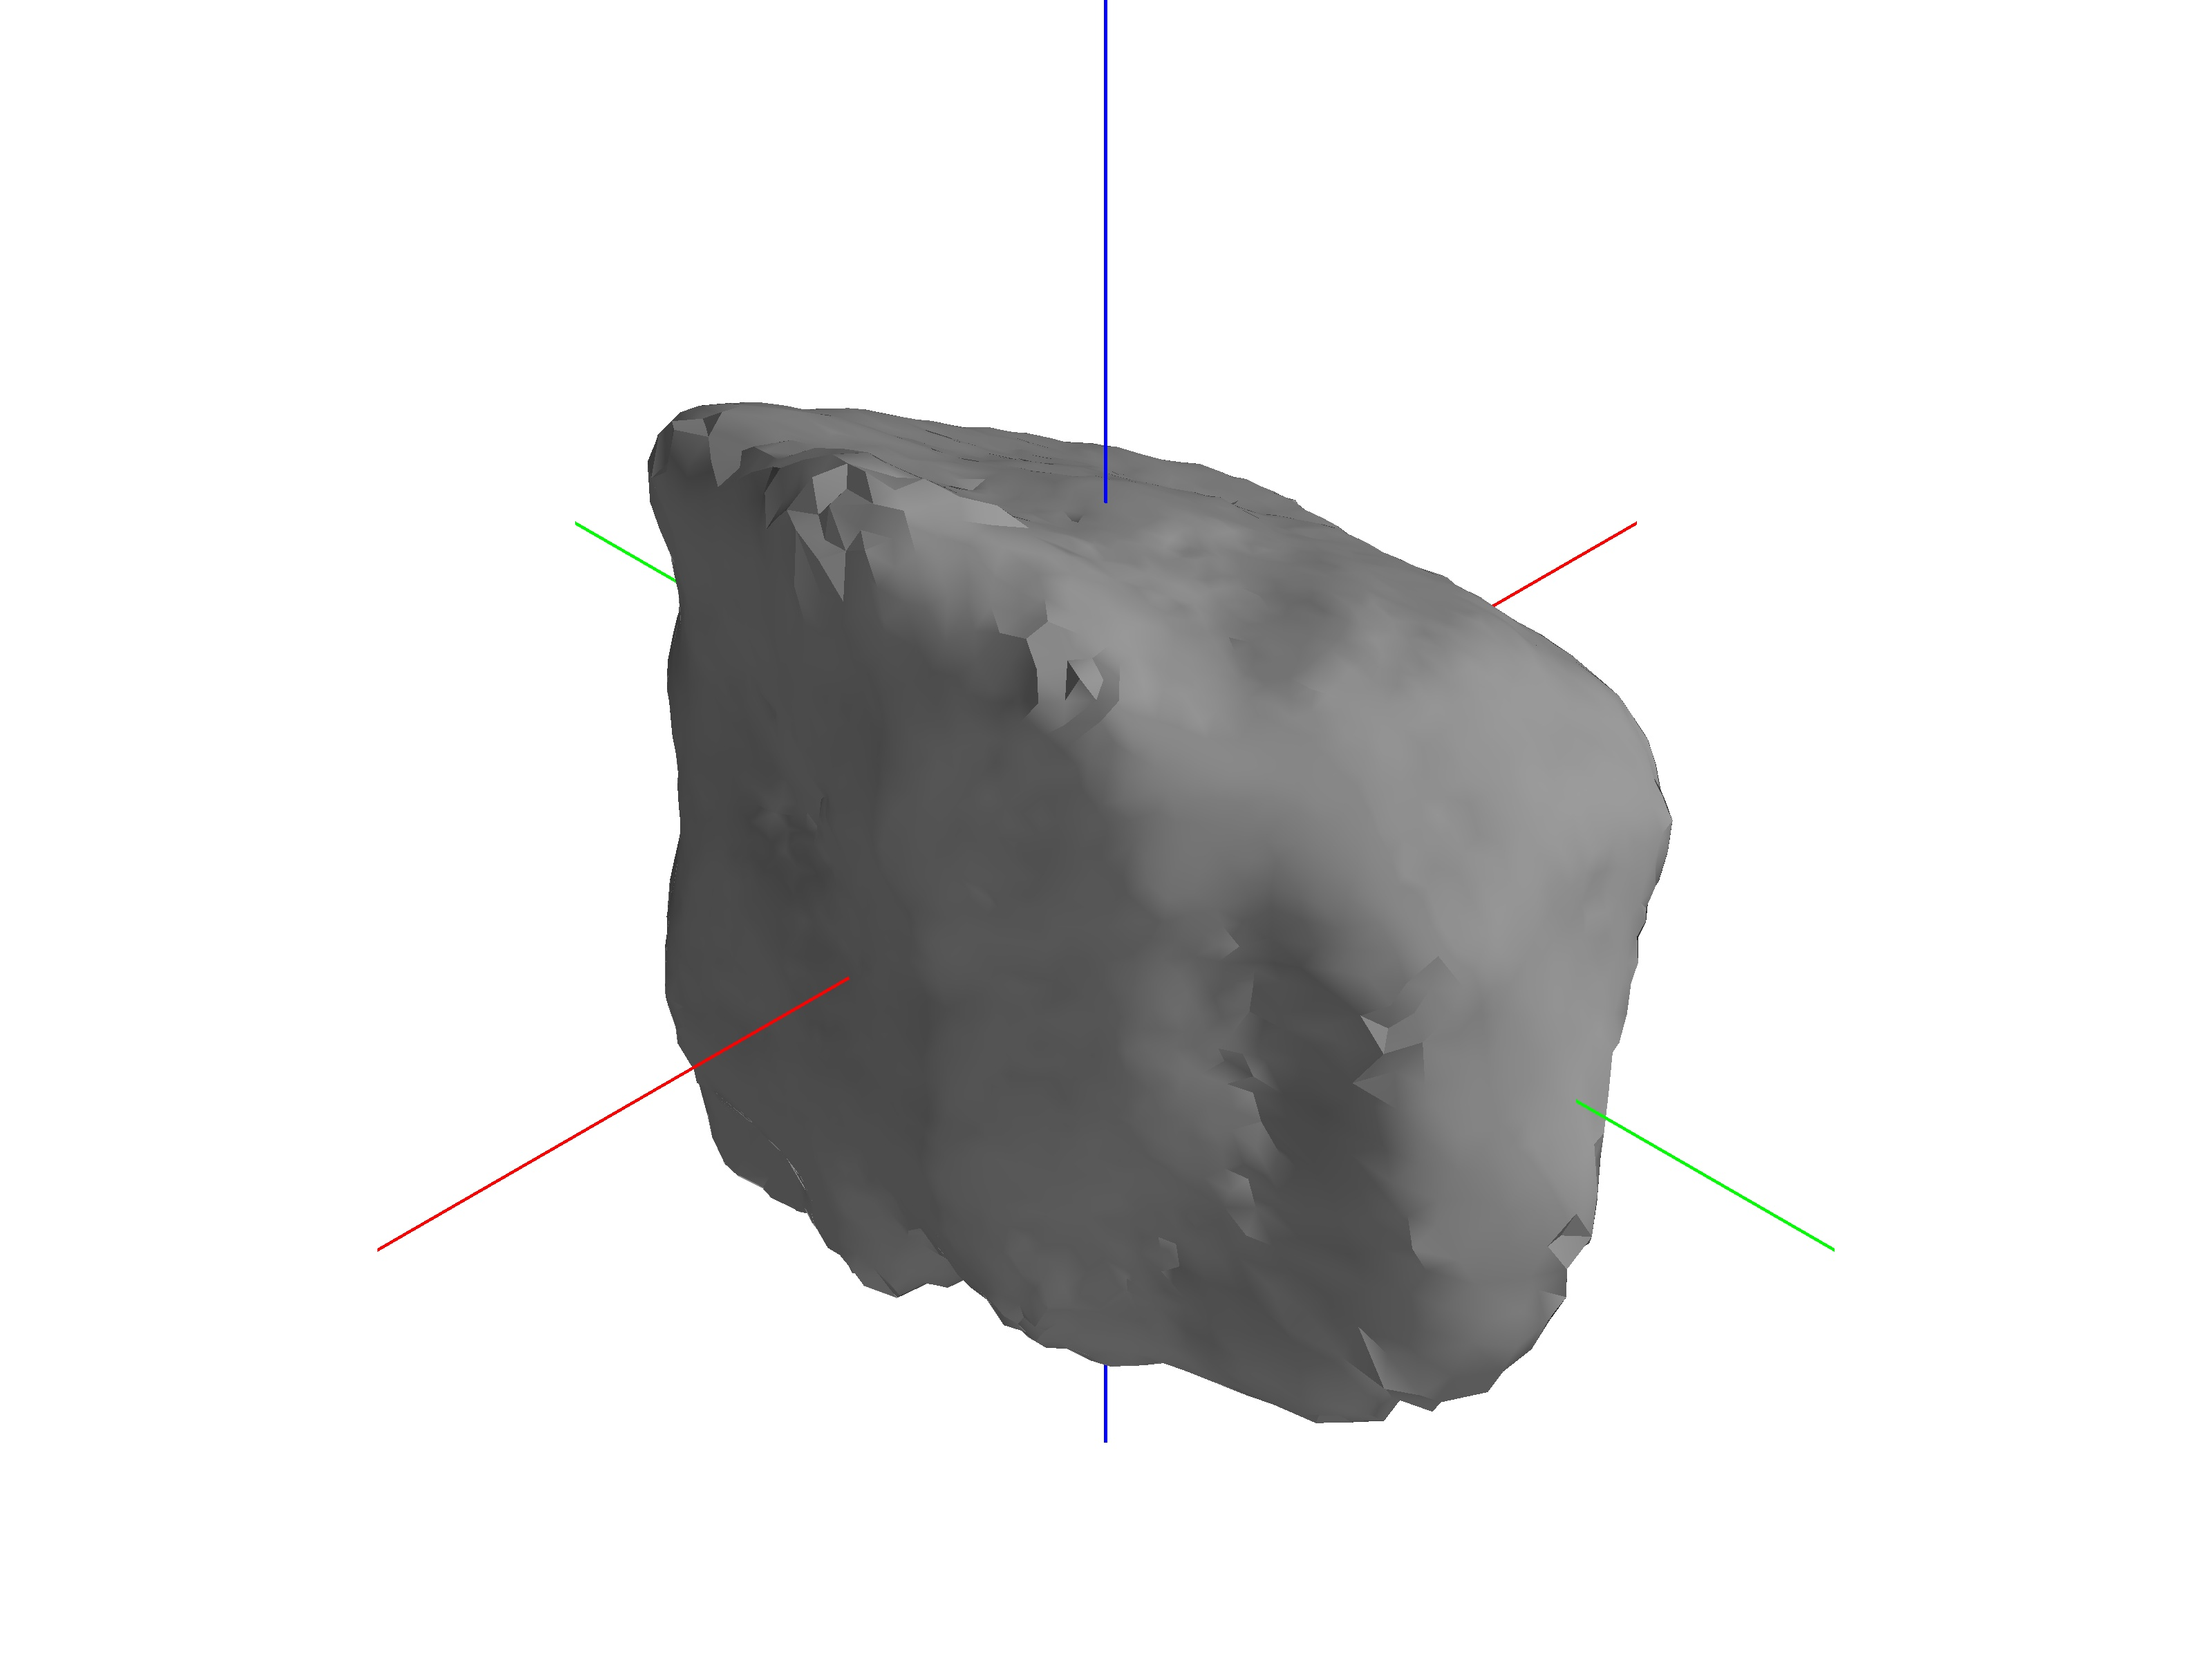
\includegraphics[trim={20cm 10cm 20cm 10cm},clip,keepaspectratio,width=0.5\textwidth,height=0.25\textheight]{figures/mesh_update/golevka/partial_2643.jpg}}%
    \subcaptionbox{\SI{75}{\percent} of measurements added\label{fig:golevka_partial_75}}{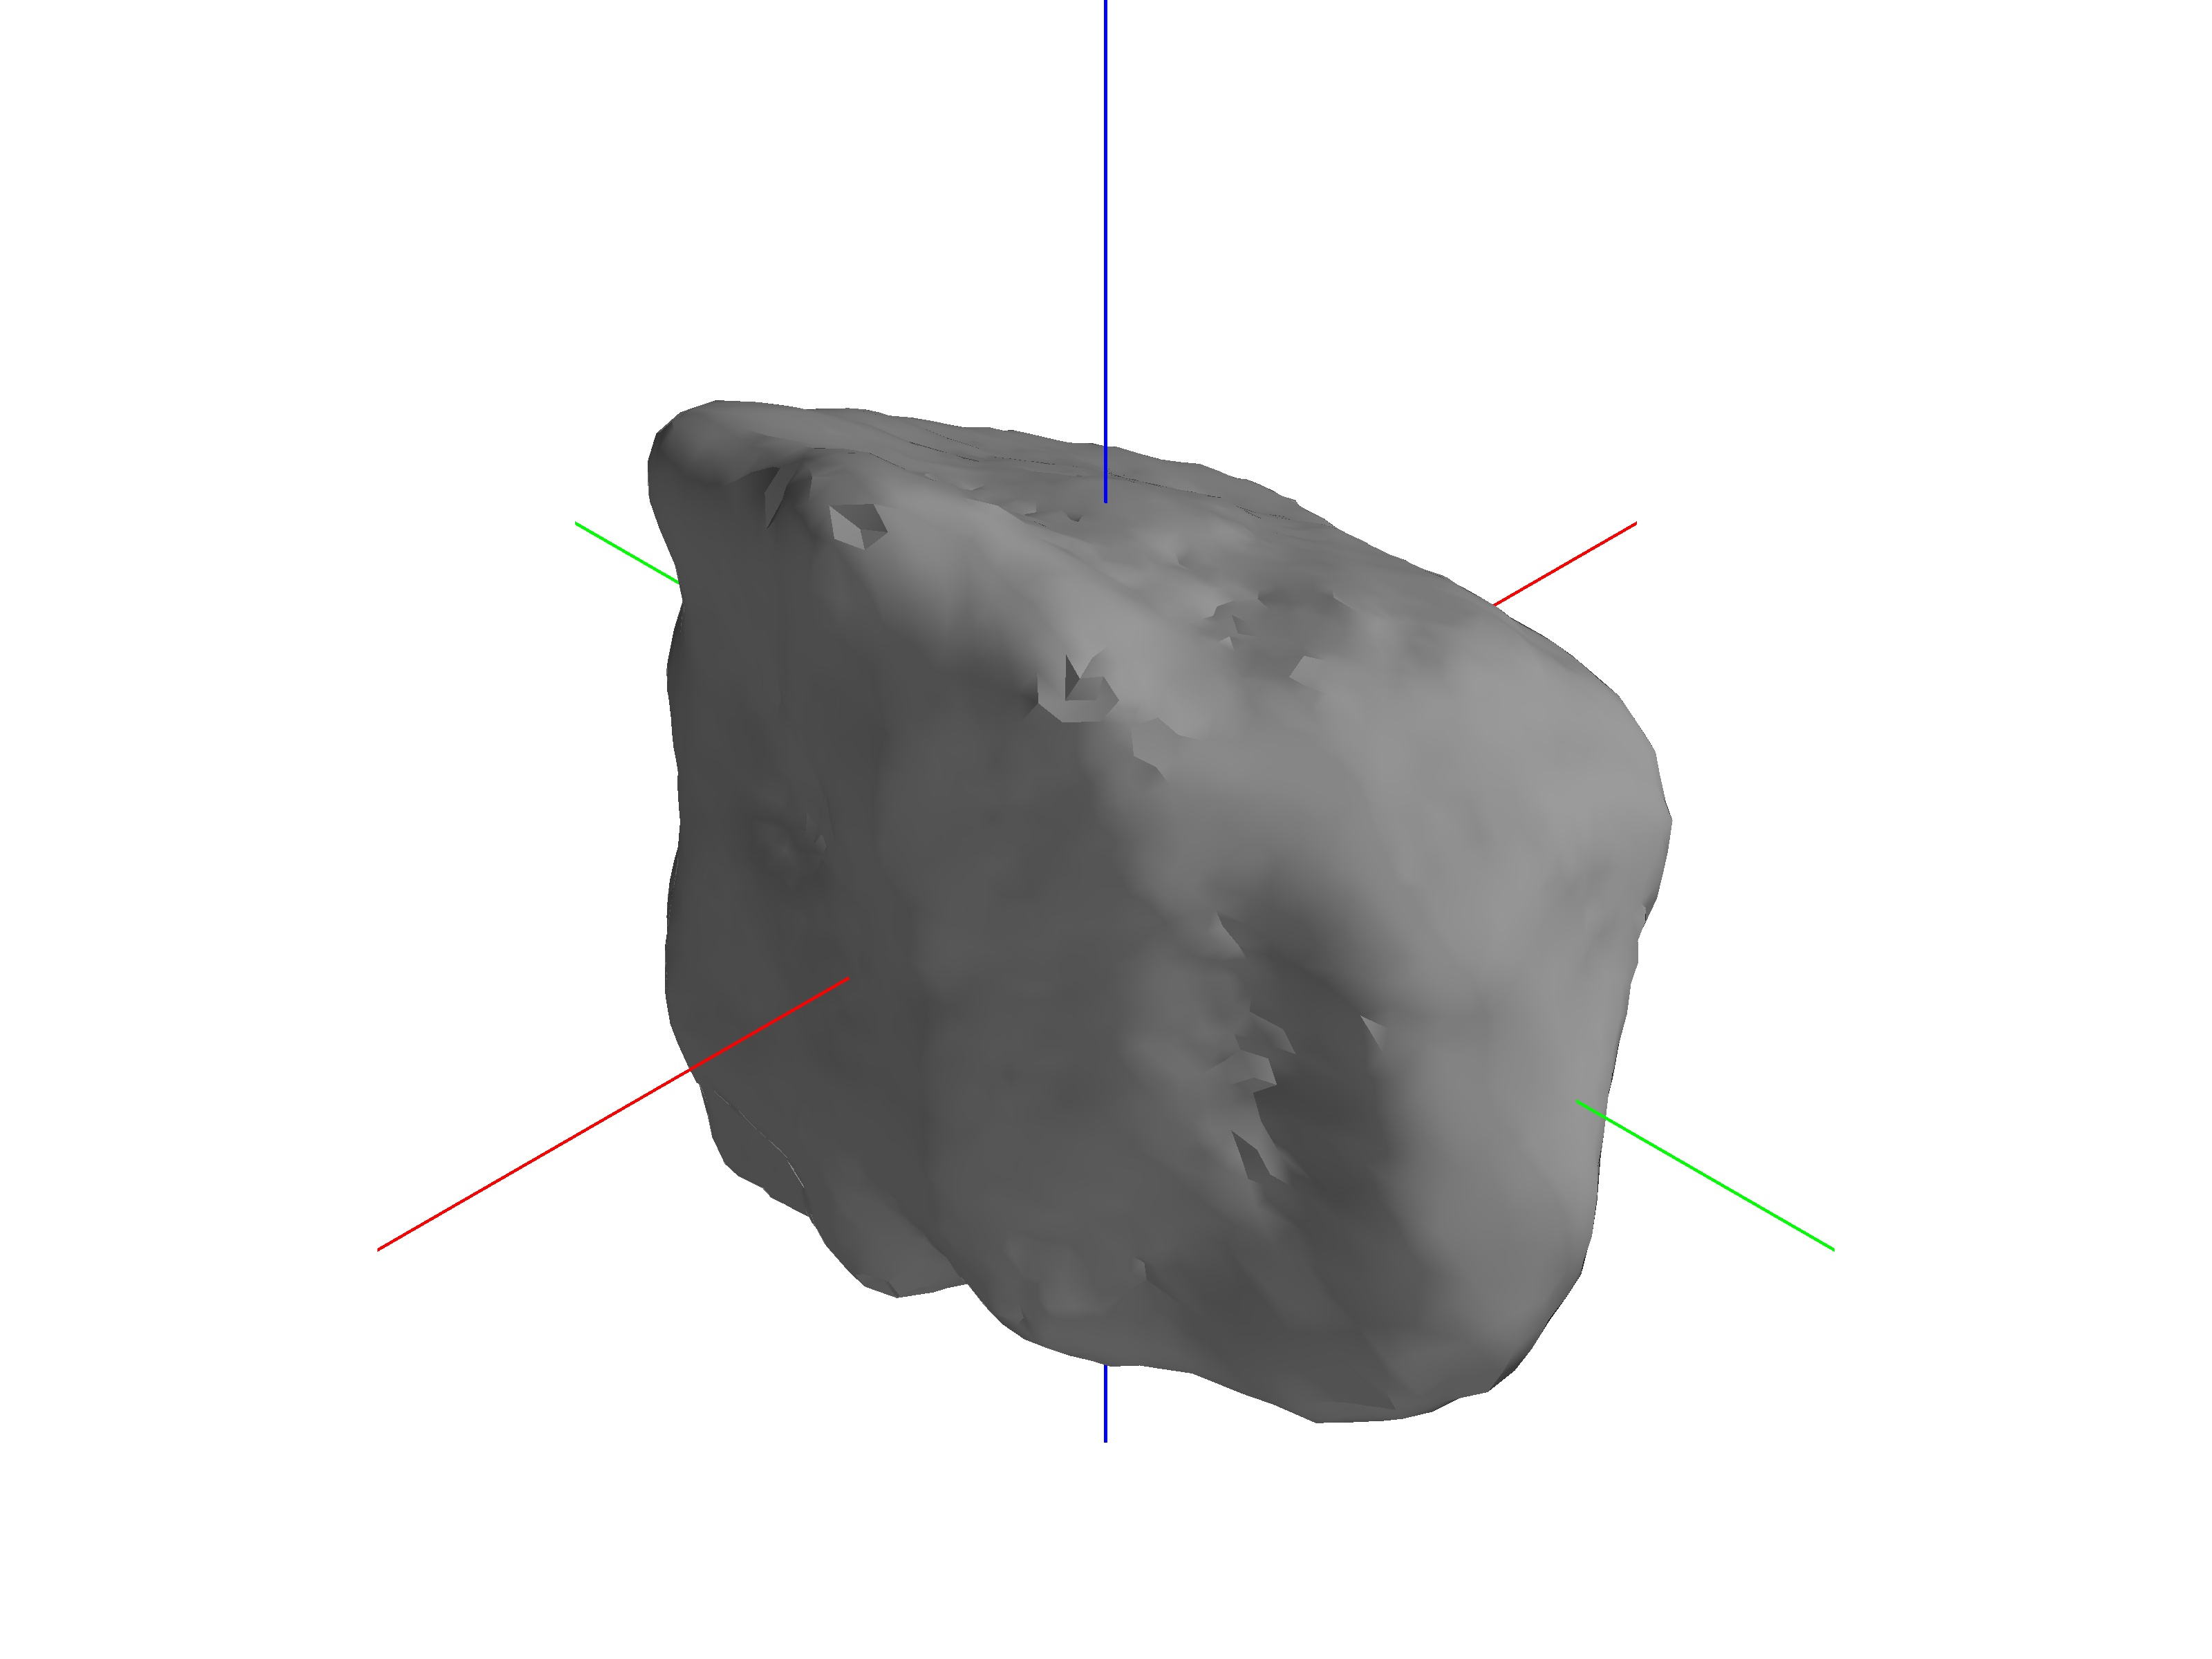
\includegraphics[trim={20cm 10cm 20cm 10cm},clip,keepaspectratio,width=0.5\textwidth,height=0.25\textheight]{figures/mesh_update/golevka/partial_3964.jpg}}\\%

    \subcaptionbox{\SI{100}{\percent} of measurements added\label{fig:golevka_partial_100}}{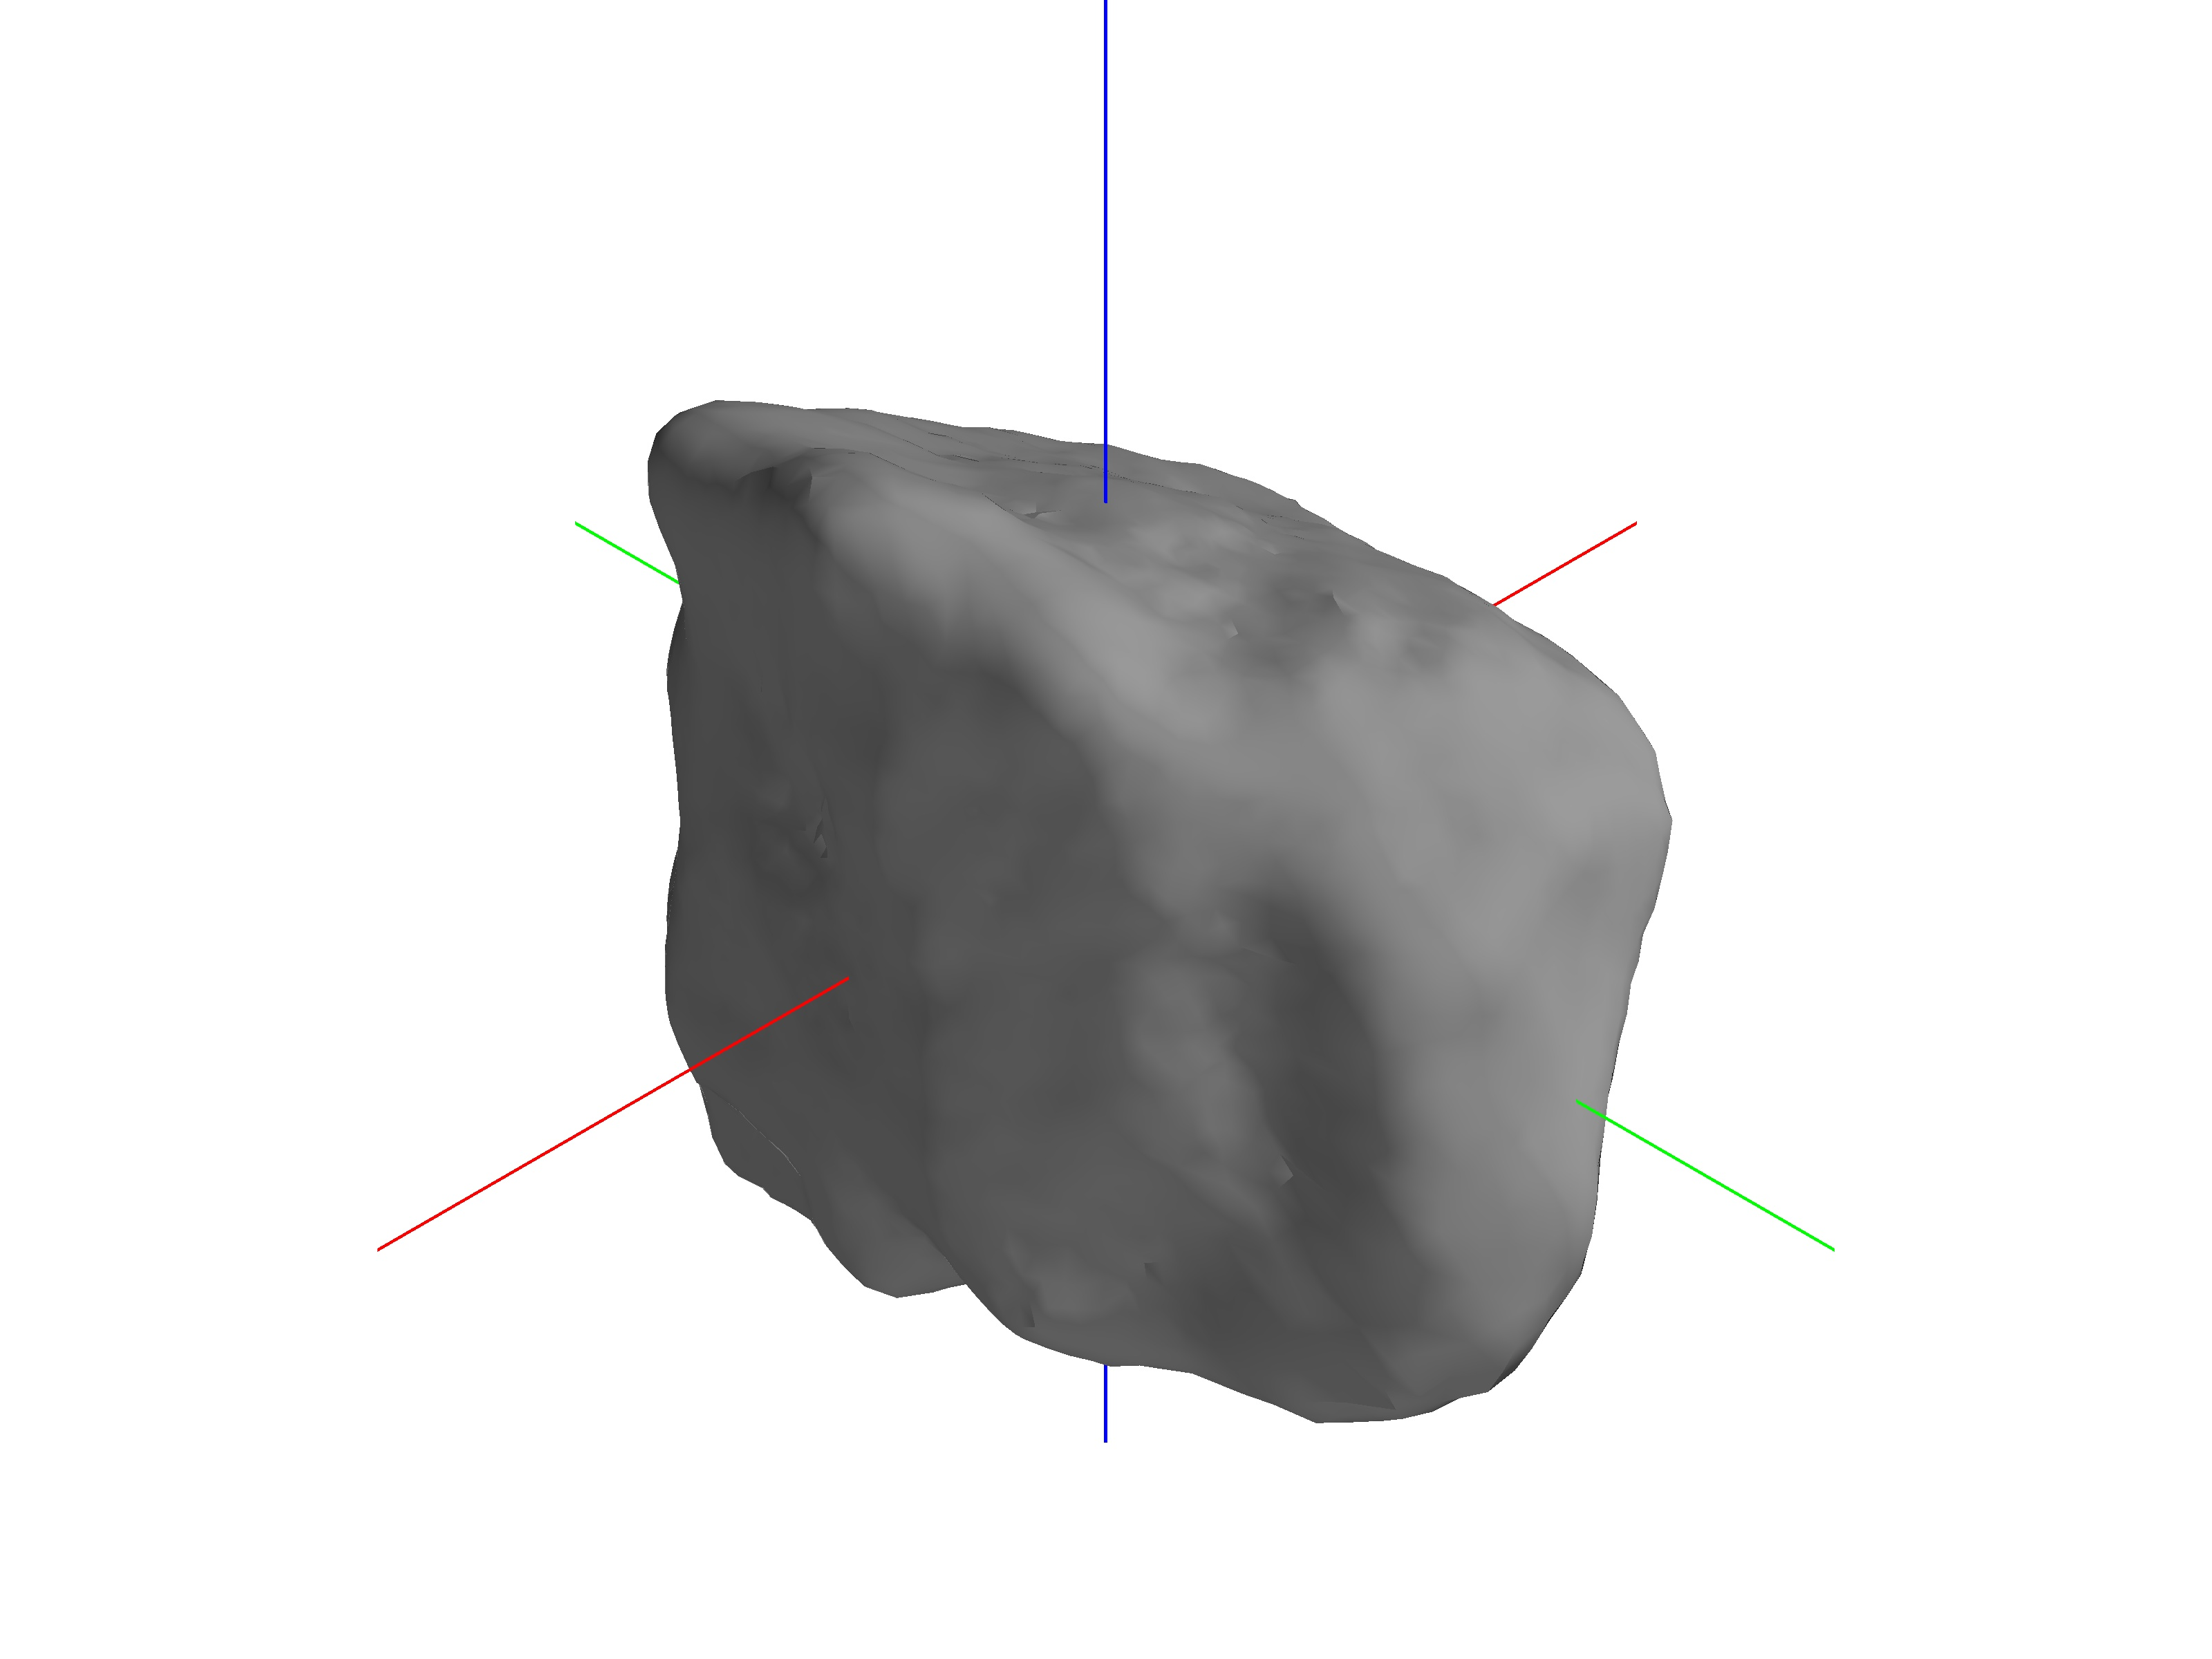
\includegraphics[trim={20cm 10cm 20cm 10cm},clip,keepaspectratio,width=0.5\textwidth,height=0.25\textheight]{figures/mesh_update/golevka/partial_5285.jpg}}%
    \subcaptionbox{True Shape Model\label{fig:golevka_truth}}{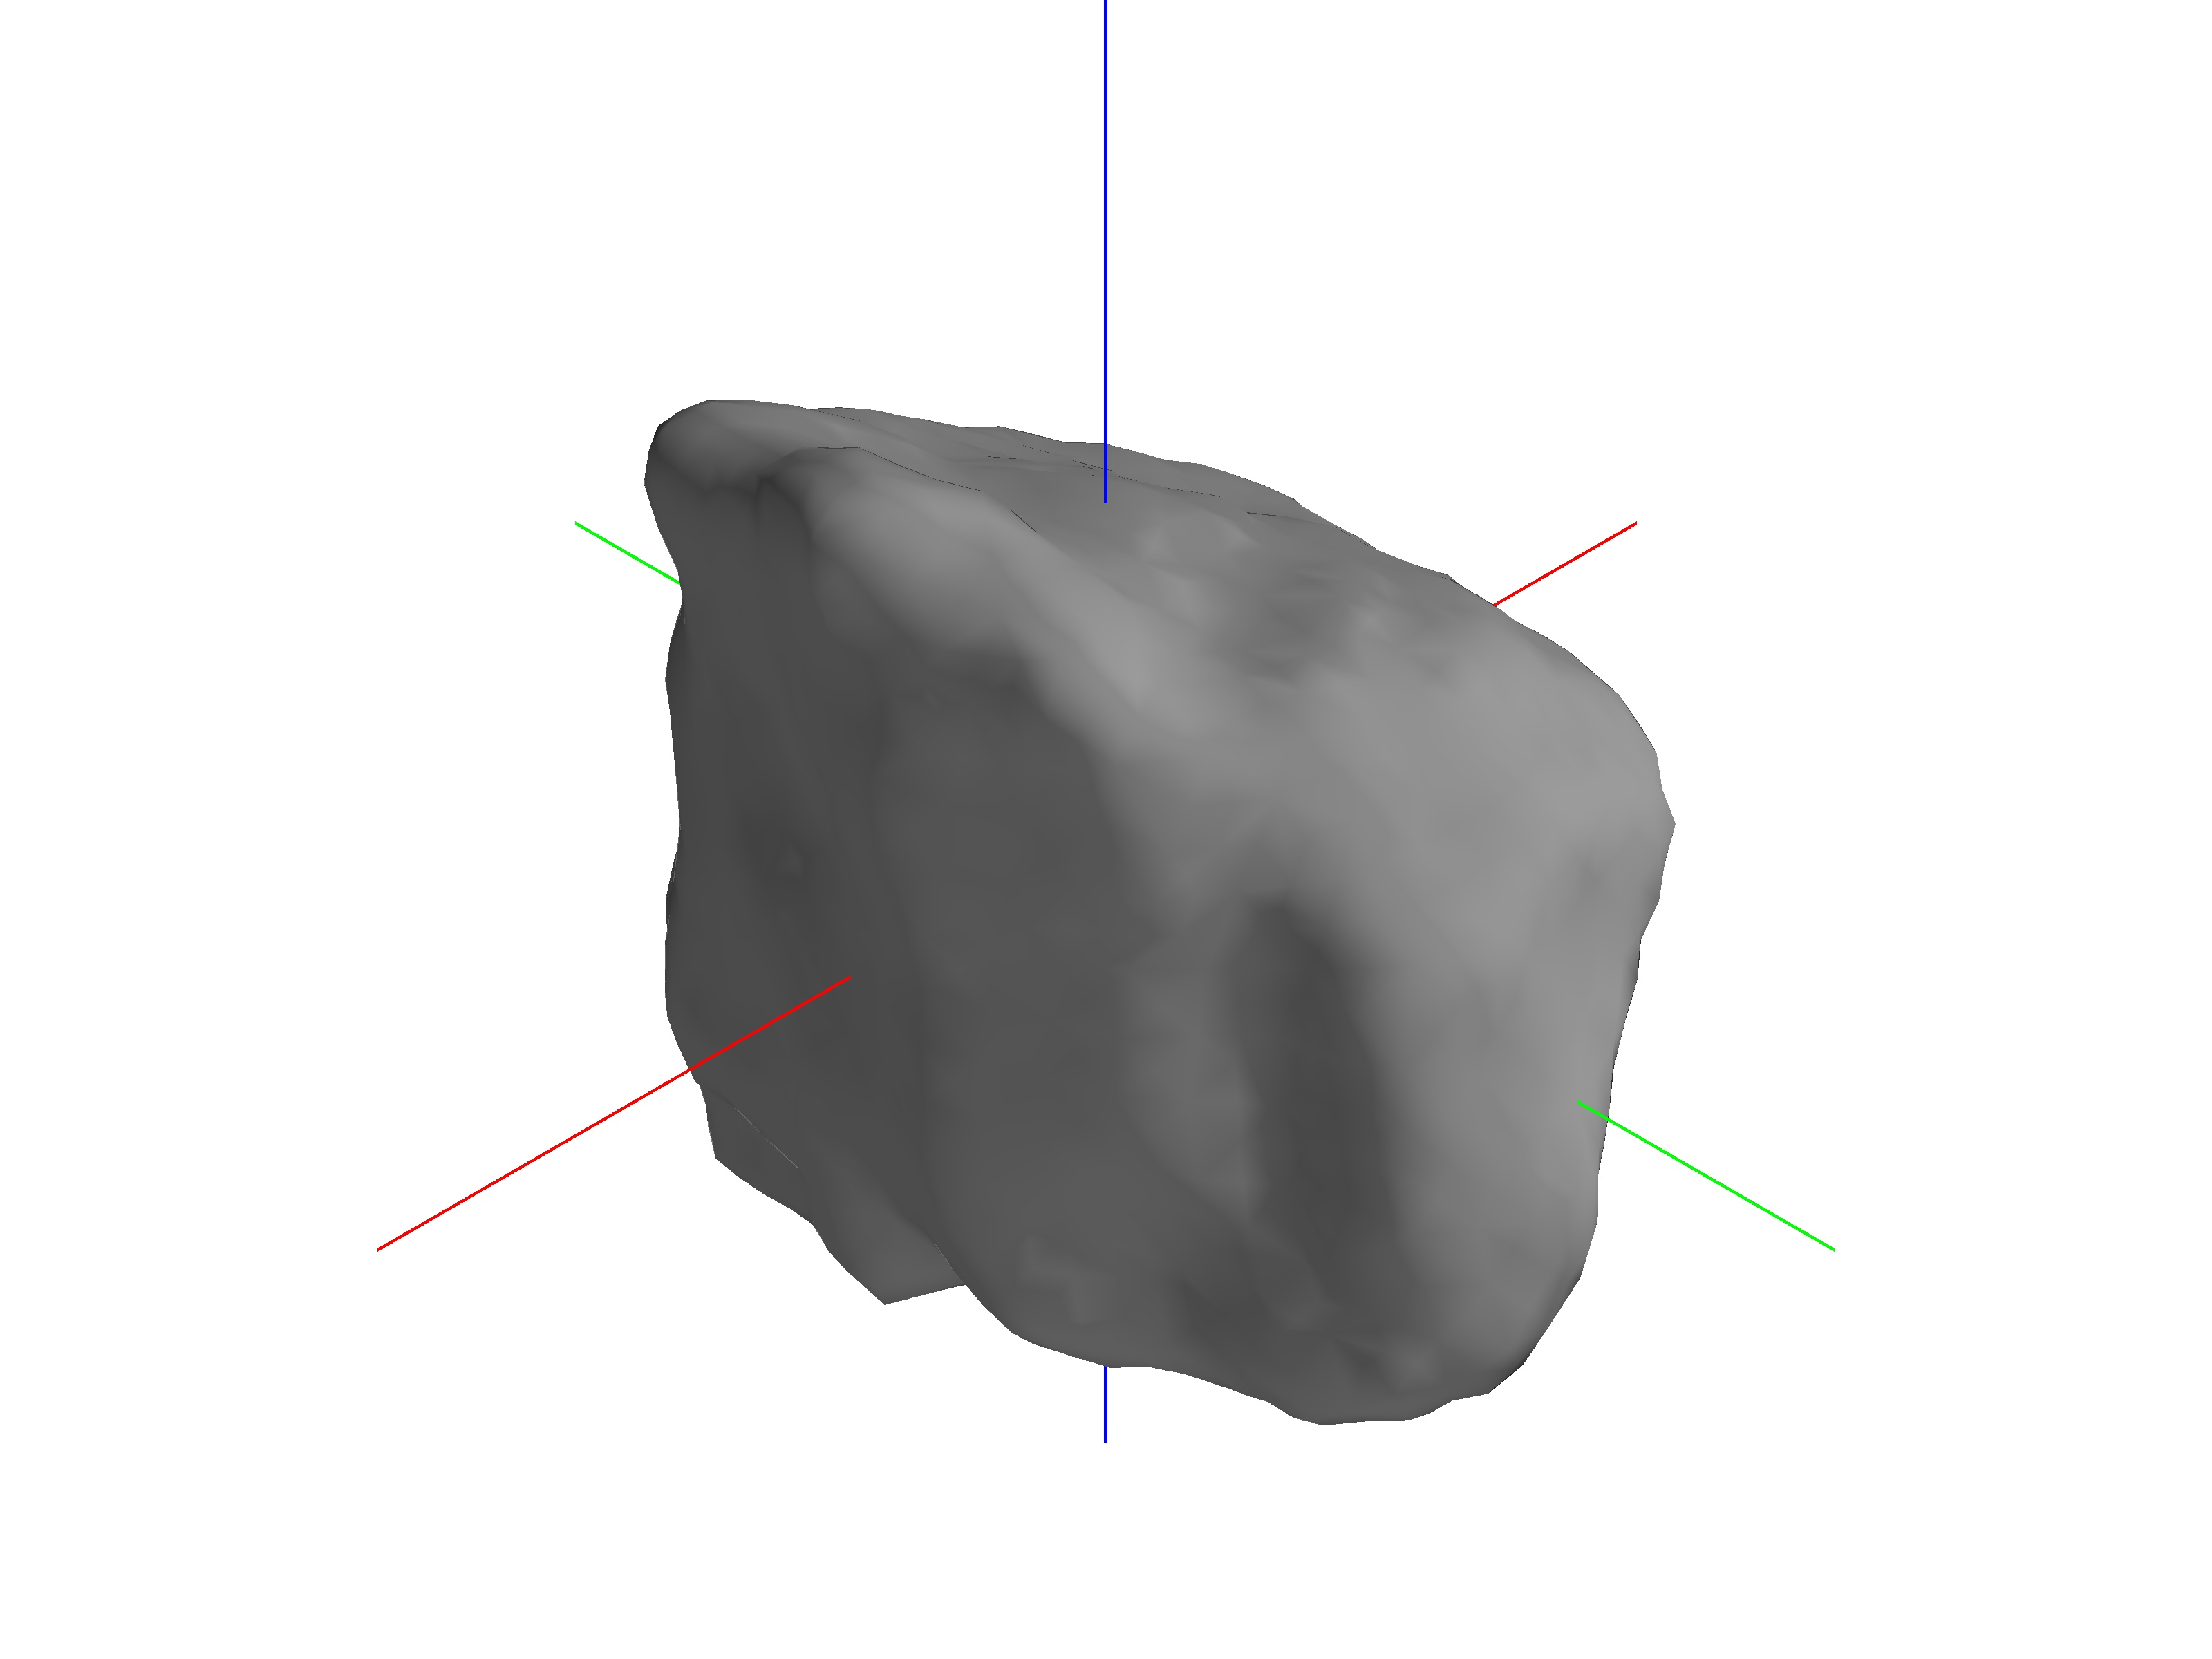
\includegraphics[trim={20cm 10cm 20cm 10cm},clip,keepaspectratio,width=0.5\textwidth,height=0.25\textheight]{figures/mesh_update/golevka/truth.jpg}}
    \caption[Asteroid Golevka incremental reconstruction]{Incremental reconstruction of asteroid Golevka~\label{fig:golevka_reconstruction}}
\end{figure}
Comparing~\cref{fig:golevka_partial_100,fig:golevka_truth} shows that the final shape closely matches the true radar model.
In~\cref{fig:golevka_metrics} we display the vertex uncertainty and mesh volume as a function of time.

\begin{figure}[htbp]
    \centering
    \tikzsetnextfilename{golevka_metrics}
\begin{tikzpicture}[baseline]
    \begin{groupplot}[
        group style={
            group name={golevka_metrics},
            group size=1 by 2,
            xlabels at=edge bottom,
            ylabels at=edge left,
            xticklabels at=edge bottom,
        },
        xlabel={Normalized Time},
        scale only axis,
        width=0.8\textwidth,
        height=0.1\textheight,
        ylabel style={align=center},
    ]
    \nextgroupplot[ylabel={Normalized\\Uncertainty}]
    \addplot [ultra thick, color=blue, mark=none] table [x=NORMALIZED_TIME, y=NORMALIZED_UNCERTAINTY, col sep=comma] {figures/mesh_update/golevka/uncertainty.csv};
    \addplot [ultra thick,red, mark=none, dashed] coordinates {
        (0.0, 0.0) (1.0, 0.0) 
    };

    \nextgroupplot[ylabel={Volume Percent\\Error}]
    \addplot [ultra thick, blue, mark=none] table [x=NORMALIZED_TIME, y=VOLUME_PERCENT_ERROR, col sep=comma] {figures/mesh_update/golevka/volume.csv};
        \addplot [ultra thick,red, mark=none, dashed] coordinates {
            (0.0, 0.0) (1.0, 0.0) 
        };
\end{groupplot}
\end{tikzpicture}


    \caption{Normalized uncertainty and volume percent error for Golevka\label{fig:golevka_metrics}}
\end{figure}

The plots show that the reconstruction achieves an accurate shape estimate with a total volume which closely matches the true volume.
It is interesting to note that the reconstruction of Golevka achieves an accurate shape reconstruction in a much smaller amount of time as compared to Geographos.
This is primarily due to the smaller size of Golevka and the relatively spherical shape of the body in contrast to the highly elliptical shape of Geographos.

\clearpage\newpage
\section{Optimal Guidance for Shape Reconstruction}\label{sec:explore_asteroid}

The shape reconstruction algorithm presented in the preceding section does not offer a method to determine which portion of the surface needs to be measured. 
In this section, we present a guidance scheme or a motion planning scheme in order to direct the spacecraft into the most uncertain region. 
This is to reduce the shape uncertainty in an optimal fashion while considering the control cost to change the orbital properties of the spacecraft. 
Then, a nonlinear geometric controller is utilized which allows the spacecraft to maneuver to the optimized location that will update the shape estimate~\cite{kulumani2017b}.

\subsection{Optimal Guidance}

We define a cost associated with each vertex \( \vc{v}_i \) of the shape estimate as
\begin{align}\label{eq:explore_cost}
    J_i (x, R, R_A) = \alpha_w J_{w_i} + \alpha_d J_{d_i}(x_r) + \alpha_c J_{c_i}(x_r)
\end{align}
where the weighting factors \( \alpha_w, \alpha_d, \alpha_c \in \R^1 \) are chosen such that \( \alpha_w + \alpha_d + \alpha_c = 1 \).
The cost function is defined as a function of the current inertial position, \( x \in \R^3 \), and the attitude, \( R \in \R^{3\times3}\) of the spacecraft.
Furthermore, knowledge of the small body rotation is required in order to determine the position of the spacecraft in the small body fixed frame, \( x_r = R_A^T x\).

The term \( J_{w_i} \in \R^1 \) represents the cost associated with the uncertainty of vertex \( i \) as
\begin{align}\label{eq:weight_cost}
    J_{w_i} &= - \frac{w_i}{w_m}
\end{align}
where \( w_i \) is the uncertainty of vertex \( i \), which is defined as the variance of the radius in the preceding section, and \( w_m \in\Re \) is a maximum uncertainty used to scale the values.
The term \( J_{d_i} \) represents the scaled geodesic distance between the current state of the spacecraft and vertex \( i \),
\begin{align}\label{eq:distance_cost}
    J_{d_i}(\rpos) &= \frac{1}{\pi} \arctan \parenth{ \frac{\norm{\rpos \times \vc{v}_i}}{\rpos \cdot \vc{v}_i}}.
\end{align}

Finally, a control component is included in the cost function which penalizes vertices that are difficult to reach.
Consider, the current position of the spacecraft in the small body fixed frame as \( \rpos\) and a desired vertex \( \vc{v}_i \) of the shape estimate.
We can define a normal vector to the plane spanned by \( \rpos, \vc{v}_i \) as
\begin{align}\label{eq:normal_to_plane}
    \vc{n}_i = \frac{\rpos \times \vc{v}_i}{\norm{\rpos} \norm{\vc{v}_i}}.
\end{align}
Then a desired trajectory \( x_d(\theta) \) as
\begin{align}\label{eq:spherical_waypoint}
    x_d(\theta) = r_d \exp{\parenth{\theta \hat{\vc{n}_i}} } \frac{\rpos}{\norm{\rpos}},
\end{align}
where \( \theta : \bracket{0, \frac{\rpos \cdot \vc{v}_i}{\norm{\rpos}\norm{\vc{v}_i}}} \to \R^1\) parameterizes the desired trajectory.
\Cref{eq:spherical_waypoint} simply describes a portion of a great circle trajectory between the current state, \( \rpos \), and the desired vertex \( \vc{v}_i \)~\cite{chen2016}, with a desired radius $r_d$.
The radius of the spacecraft, \( r_d \in \R \), can be chosen based on sensor characteristics of safety concerns.
For example, \( r_d \) can be chosen as the distance of the Biroullin sphere with an additional safety margin to mitigate any surface collision~\cite{scheeres2012a}.

We assume $\theta$ varies linearly with respect to $t$, and substitute the desired trajectory into \Cref{eq:v_dot} to obtain the control force required to follow the desired trajectory in the absence of any tracking error:
\begin{align}\label{eq:tracking_control_cost}
    u_f(\theta) = -F_{ext}(x_d(\theta)), 
\end{align}
which is computed by the polyhedron potential model given in~\cref{eq:attraction}.
The control cost is then defined as the integral over the desired trajectory~\cref{eq:spherical_waypoint} between the current state and the desired vertex as
\begin{align}\label{eq:control_cost}
    J_{c_i}(\rpos) = \frac{1}{u_m} \int_{\theta_0}^{\theta_f} u_f(\theta)^T R u_f(\theta) d\theta,
\end{align}
where \( u_m \) is used to normalize and scale \( J_{c_i} \).
\Cref{eq:control_cost} is numerically integrated over the trajectory \( x_d(t) \) and used to penalize vertices which have a larger cost.

\todo{Augment dynamic model with the control force and the torque}


The vertex which minimizes~\cref{eq:explore_cost} 
\begin{align*}
    \vc{v}_{min} = \argmin_{i} \{J_i(x, R, R_A)\},
\end{align*}
is determined.
This vertex is then used to determine the desired trajectory of the spacecraft in order to collect a measurement as in~\Cref{eq:spherical_waypoint}.

Next, the desired attitude command, \( R_d\), is chosen such that the spacecraft camera axis, \( \vc{b}_1 \), is directed along the nadir towards the asteroid.
It is sufficient to define two orthogonal vectors to uniquely determine the attitude of the spacecraft.
The \( \vc{b}_{3d} \) vector is chosen to lie in the plane spanned by \(\vc{b}_{1d} \) and \( \vc{e}_3 = \vc{f}_3 \).
The desired attitude command is defined as
\begin{align}
    \vc{b}_{1d} &= - \frac{\vc{x}}{\norm{\vc{x}}} , \\
    \vc{b}_{3d} &= \frac{\vc{f}_3 - \parenth{\vc{f}_3 \cdot \vc{b}_{1d}} \vc{b}_{1d}}{\norm{\vc{f}_3 - \parenth{\vc{f}_3 \cdot \vc{b}_{1d}} \vc{b}_{1d}}}, \\
    \vc{b}_{2d} &= \vc{b}_{3d} \times \vc{b}_{1d} , \\
    R_d &= \begin{bmatrix} \vc{b}_{1d} & \vc{b}_{2d} & \vc{b}_{3d} \end{bmatrix} .
\end{align}
This form of \( R_d \) will direct the \( b_1 \) axis towards the small body, and can be modified for a different camera orientation.

\subsection{Geometric Tracking Control}

We utilize a geometric tracking control system to follow the desired trajectory for the position and the attitude defined above. 

\todo{add description of control}

\subsection{Numerical Examples}

We utilize radar shape models of asteroids \num{4769} Castalia and (\num{52760}) \num{1998} \(\text{ML}_{14}\).
The examples demonstrate the full dynamic simulation of a rigid spacecraft with an autonomous closed loop control scheme to both reconstruct the asteroid shape.
More specifically, the nonlinear controllers described previously are used to control both the translational and rotational states of the vehicle, where the control inputs are computed using the current shape estimate of the asteroid. 
As measurements are collected, the spacecraft autonomously updates its shape estimate and uses this estimate to compute the control inputs and desired future states.
As such, both the shape model and the gravitational potential available to the controller will be gradually refined. 
However, throughout the simulation, the actual spacecraft dynamics are computed with the gravity computed by the full shape model unknown to the controller.
These demonstrate the ability of a spacecraft to autonomously explore and maneuver around an initially-unknown asteroids while incrementally updating the shape model.

The asteroids are assumed to constantly rotate about the \( \vc{f}_3 = \vc{e}_3\) axis according to the parameters given in~\cref{tab:dynamic_asteroids}.
Furthermore, the state of the asteroid, namely the rotation matrix \( R_A \), is assumed to be known based on ground measurements or previous data.
\begin{table}[htbp]
    \centering
    \begin{tabular}{lcc}
        \toprule
        Property & \num{4769} Castalia & (\num{52760}) \num{1998} \(\text{ML}_{14}\) \\
        \midrule
        Semi-major axes(\si{\kilo\meter}) & \( 0.8065 \times 0.4905 \times 0.413 \) & \( 1.1 \times 1.1 \times 1.1 \) \\
        Rotational Period (\si{\hour}) & \num{4.095} & \num{14.98} \\
        Density (\si{\gram\per\centi\meter^3}) & \num{2.1} & \num{2.1} \\
        Vertices & \num{2048}  & \num{8192} \\
        Faces & \num{4092} & \num{16320} \\
        \bottomrule
    \end{tabular}
    \caption{Asteroid properties for dynamic exploration~\label{tab:dynamic_asteroids}}
\end{table}
At the beginning of the simulation the spacecraft is assumed to lie on the inertial \( e_1 \) axis, i.e.\ \( x_0 = \begin{bmatrix} x_0 & 0 & 0 \end{bmatrix} \si{\kilo\meter} \).
In addition, at the initial state the spacecraft is orientated such that the \( b_1 \) axis is aligned with the inertial \( e_2 \) axis.
In other words the initial orientation is given by \( R_0 = \exp(\frac{\pi}{2} \hat{e}_3)\).
The shape reconstruction phase of the simulation is performed over \SI{15000}{\second}, over which time the spacecraft will take LIDAR measurements of the surface at \SI{1}{\hertz}.
Once the total uncertainty has been reduced sufficiently the spacecraft maneuvers to a ``home'' position aligned with the \( f_1 \) axis of the asteroid.

\paragraph{Asteroid 52760 Reconstruction}

Asteroid (\num{52760}) \num{1998} \(\text{ML}_{14}\) was discovered in \num{1998} and is near Earth asteroid of the Apollo group and classified as a potentially hazardous body.
The asteroid is roughly spherical with a mean radius of approximately \SI{1}{\kilo\meter}.
The initial shape estimate is assumed to be spherical with approximately the same number of vertices as the truth model.
\Cref{fig:52760_weights_reconstruction} show the shape reconstruction at several discrete points during the simulation.
Due to the roughly spherical shape of the asteroid large portions of the surface are quickly modified to match the measurements.
In addition~\cref{fig:52760_weights_reconstruction} displays the vertex uncertainty \( w_i \) as a colormap on the surface. 
Areas of high uncertainty are denoted in yellow while areas of low uncertainty are in purple/blue.

\begin{figure}[htbp]
    \centering
    \subcaptionbox{Initial Shape Estimate\label{fig:52760_partial_weights_0}}{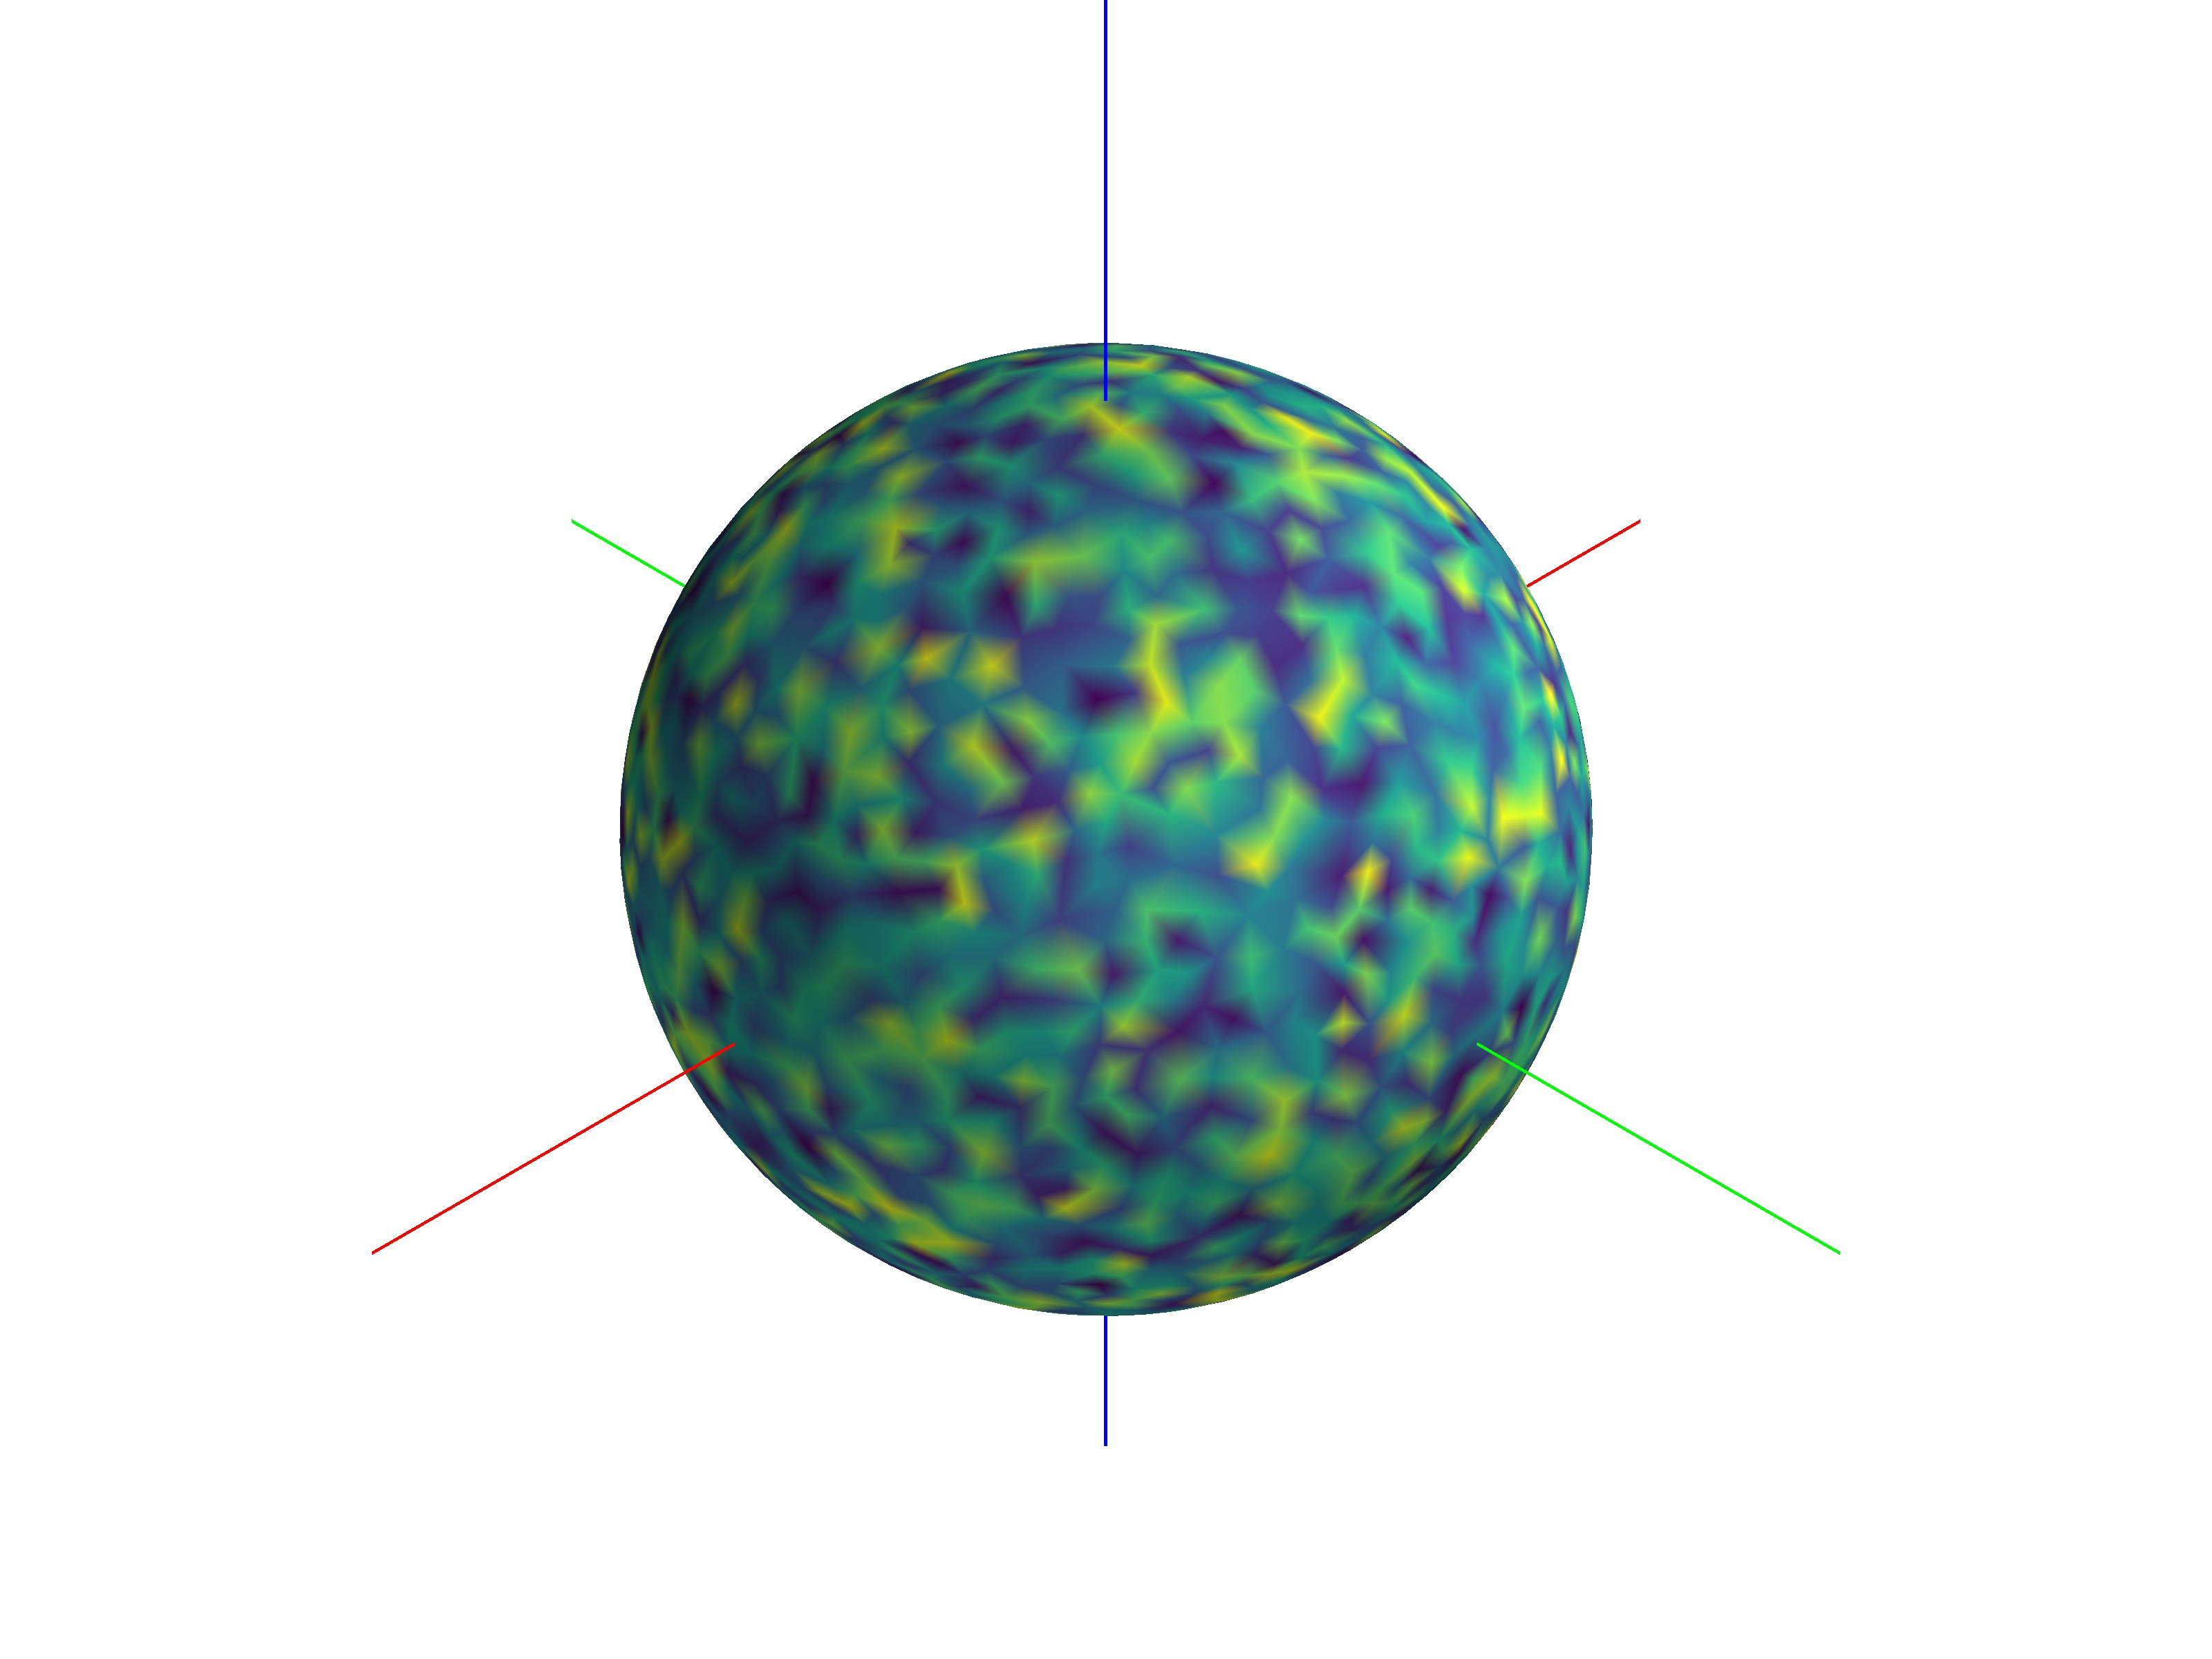
\includegraphics[trim={30cm 15cm 30cm 15cm},clip,height=0.25\textheight,width=0.5\textwidth,keepaspectratio]{figures/dynamic_exploration/52760/partial_weights_1.jpg}}%
    \subcaptionbox{\SI{25}{\percent} of measurements\label{fig:52760_partial_weights_25}}{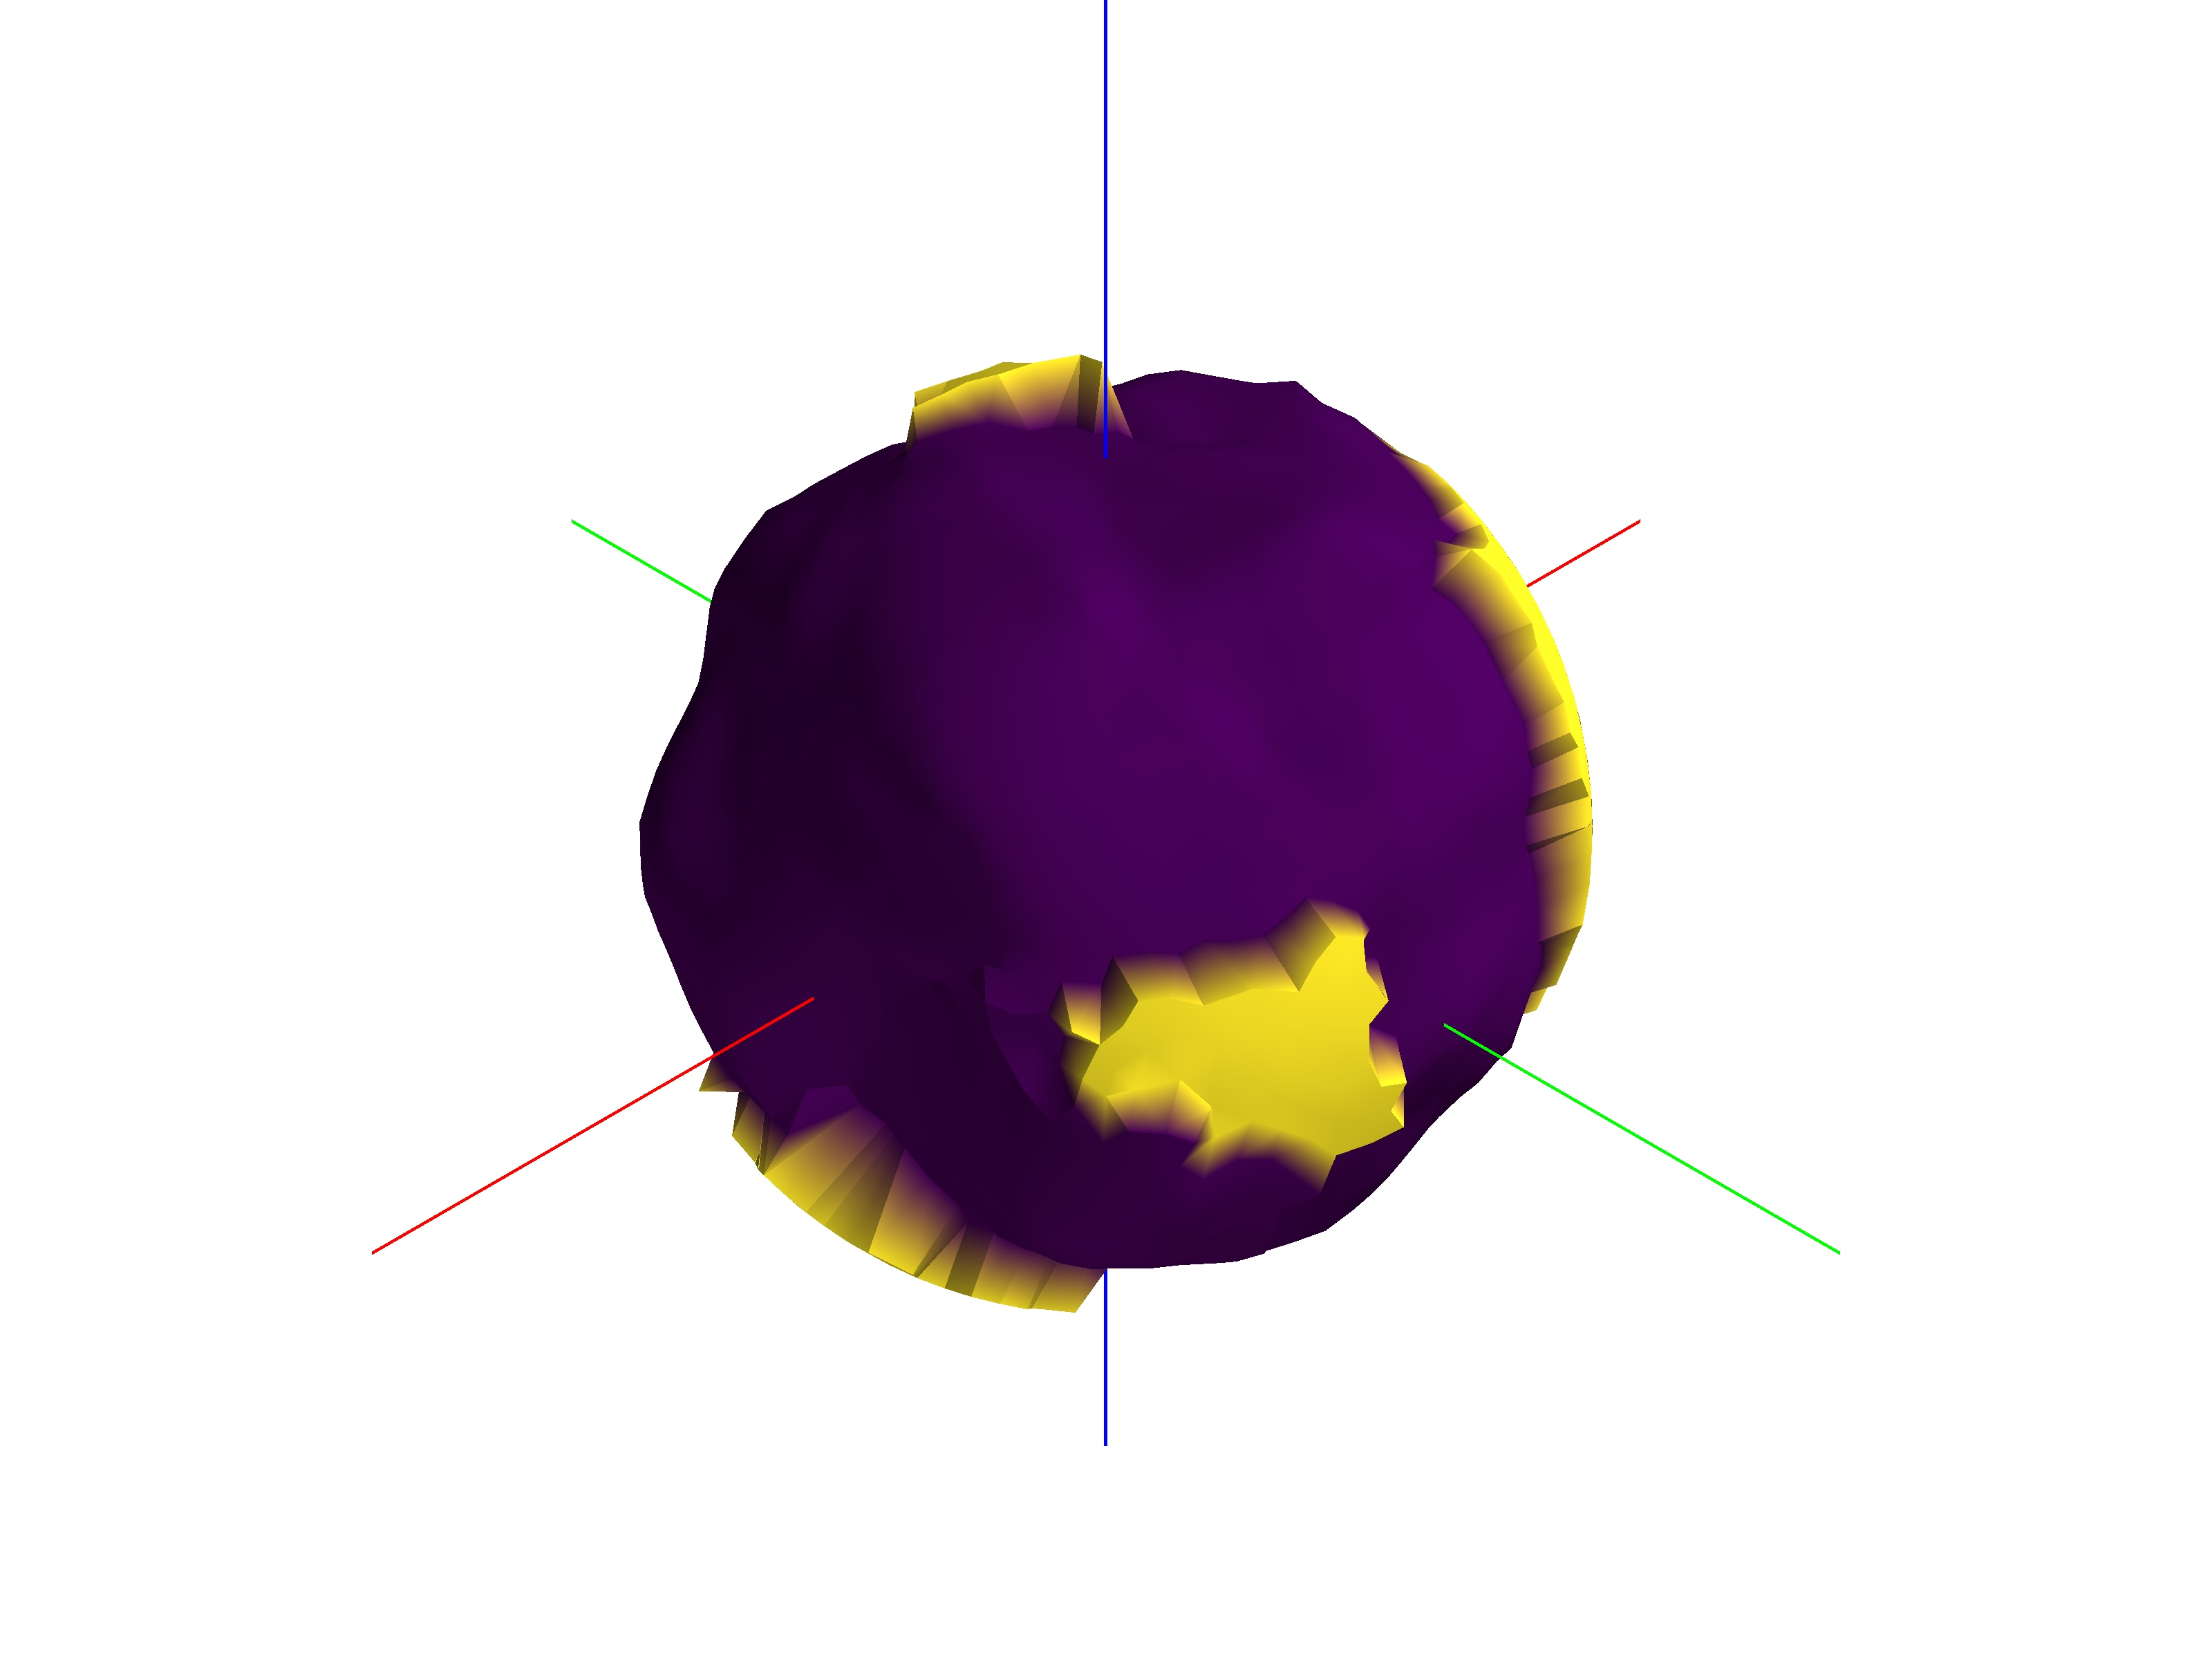
\includegraphics[trim={30cm 15cm 30cm 15cm},clip,height=0.25\textheight,width=0.5\textwidth,keepaspectratio]{figures/dynamic_exploration/52760/partial_weights_3749.jpg}}%

    \subcaptionbox{\SI{50}{\percent} of measurements\label{fig:52760_partial_weights_50}}{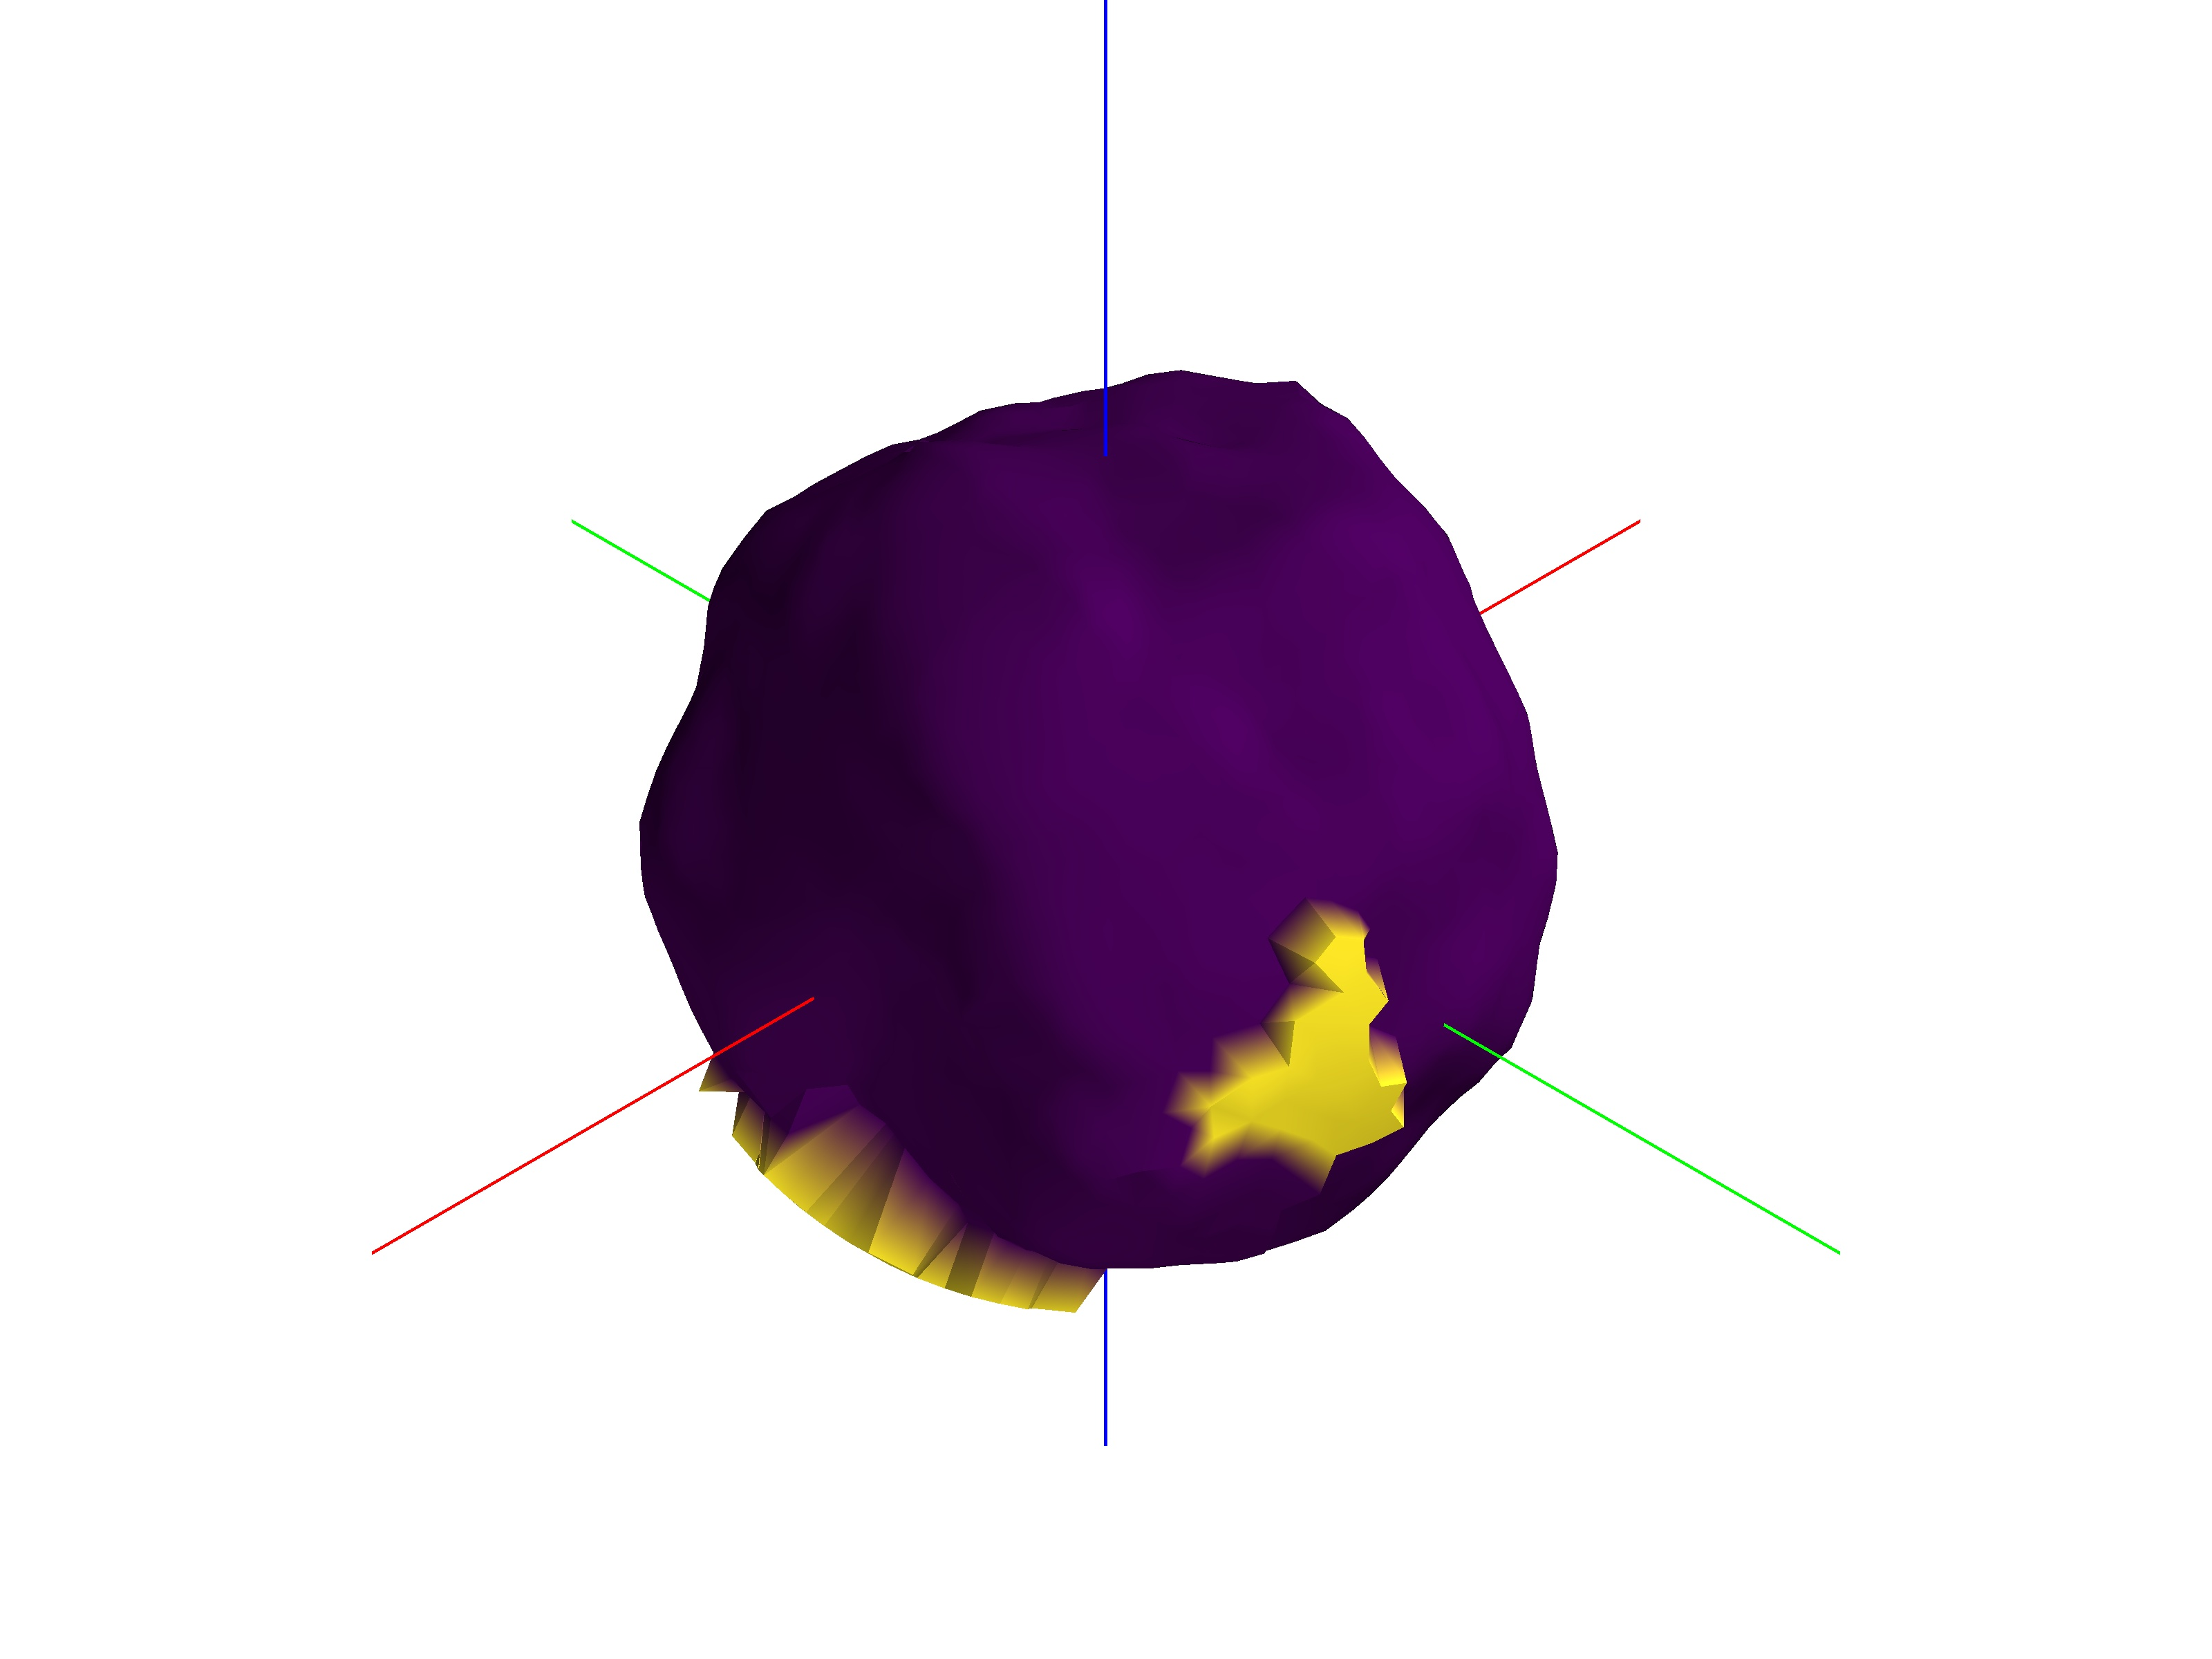
\includegraphics[trim={30cm 15cm 30cm 15cm},clip,height=0.25\textheight,width=0.5\textwidth,keepaspectratio]{figures/dynamic_exploration/52760/partial_weights_7499.jpg}}
    \subcaptionbox{\SI{75}{\percent} of measurements\label{fig:52760_partial_weights_75}}{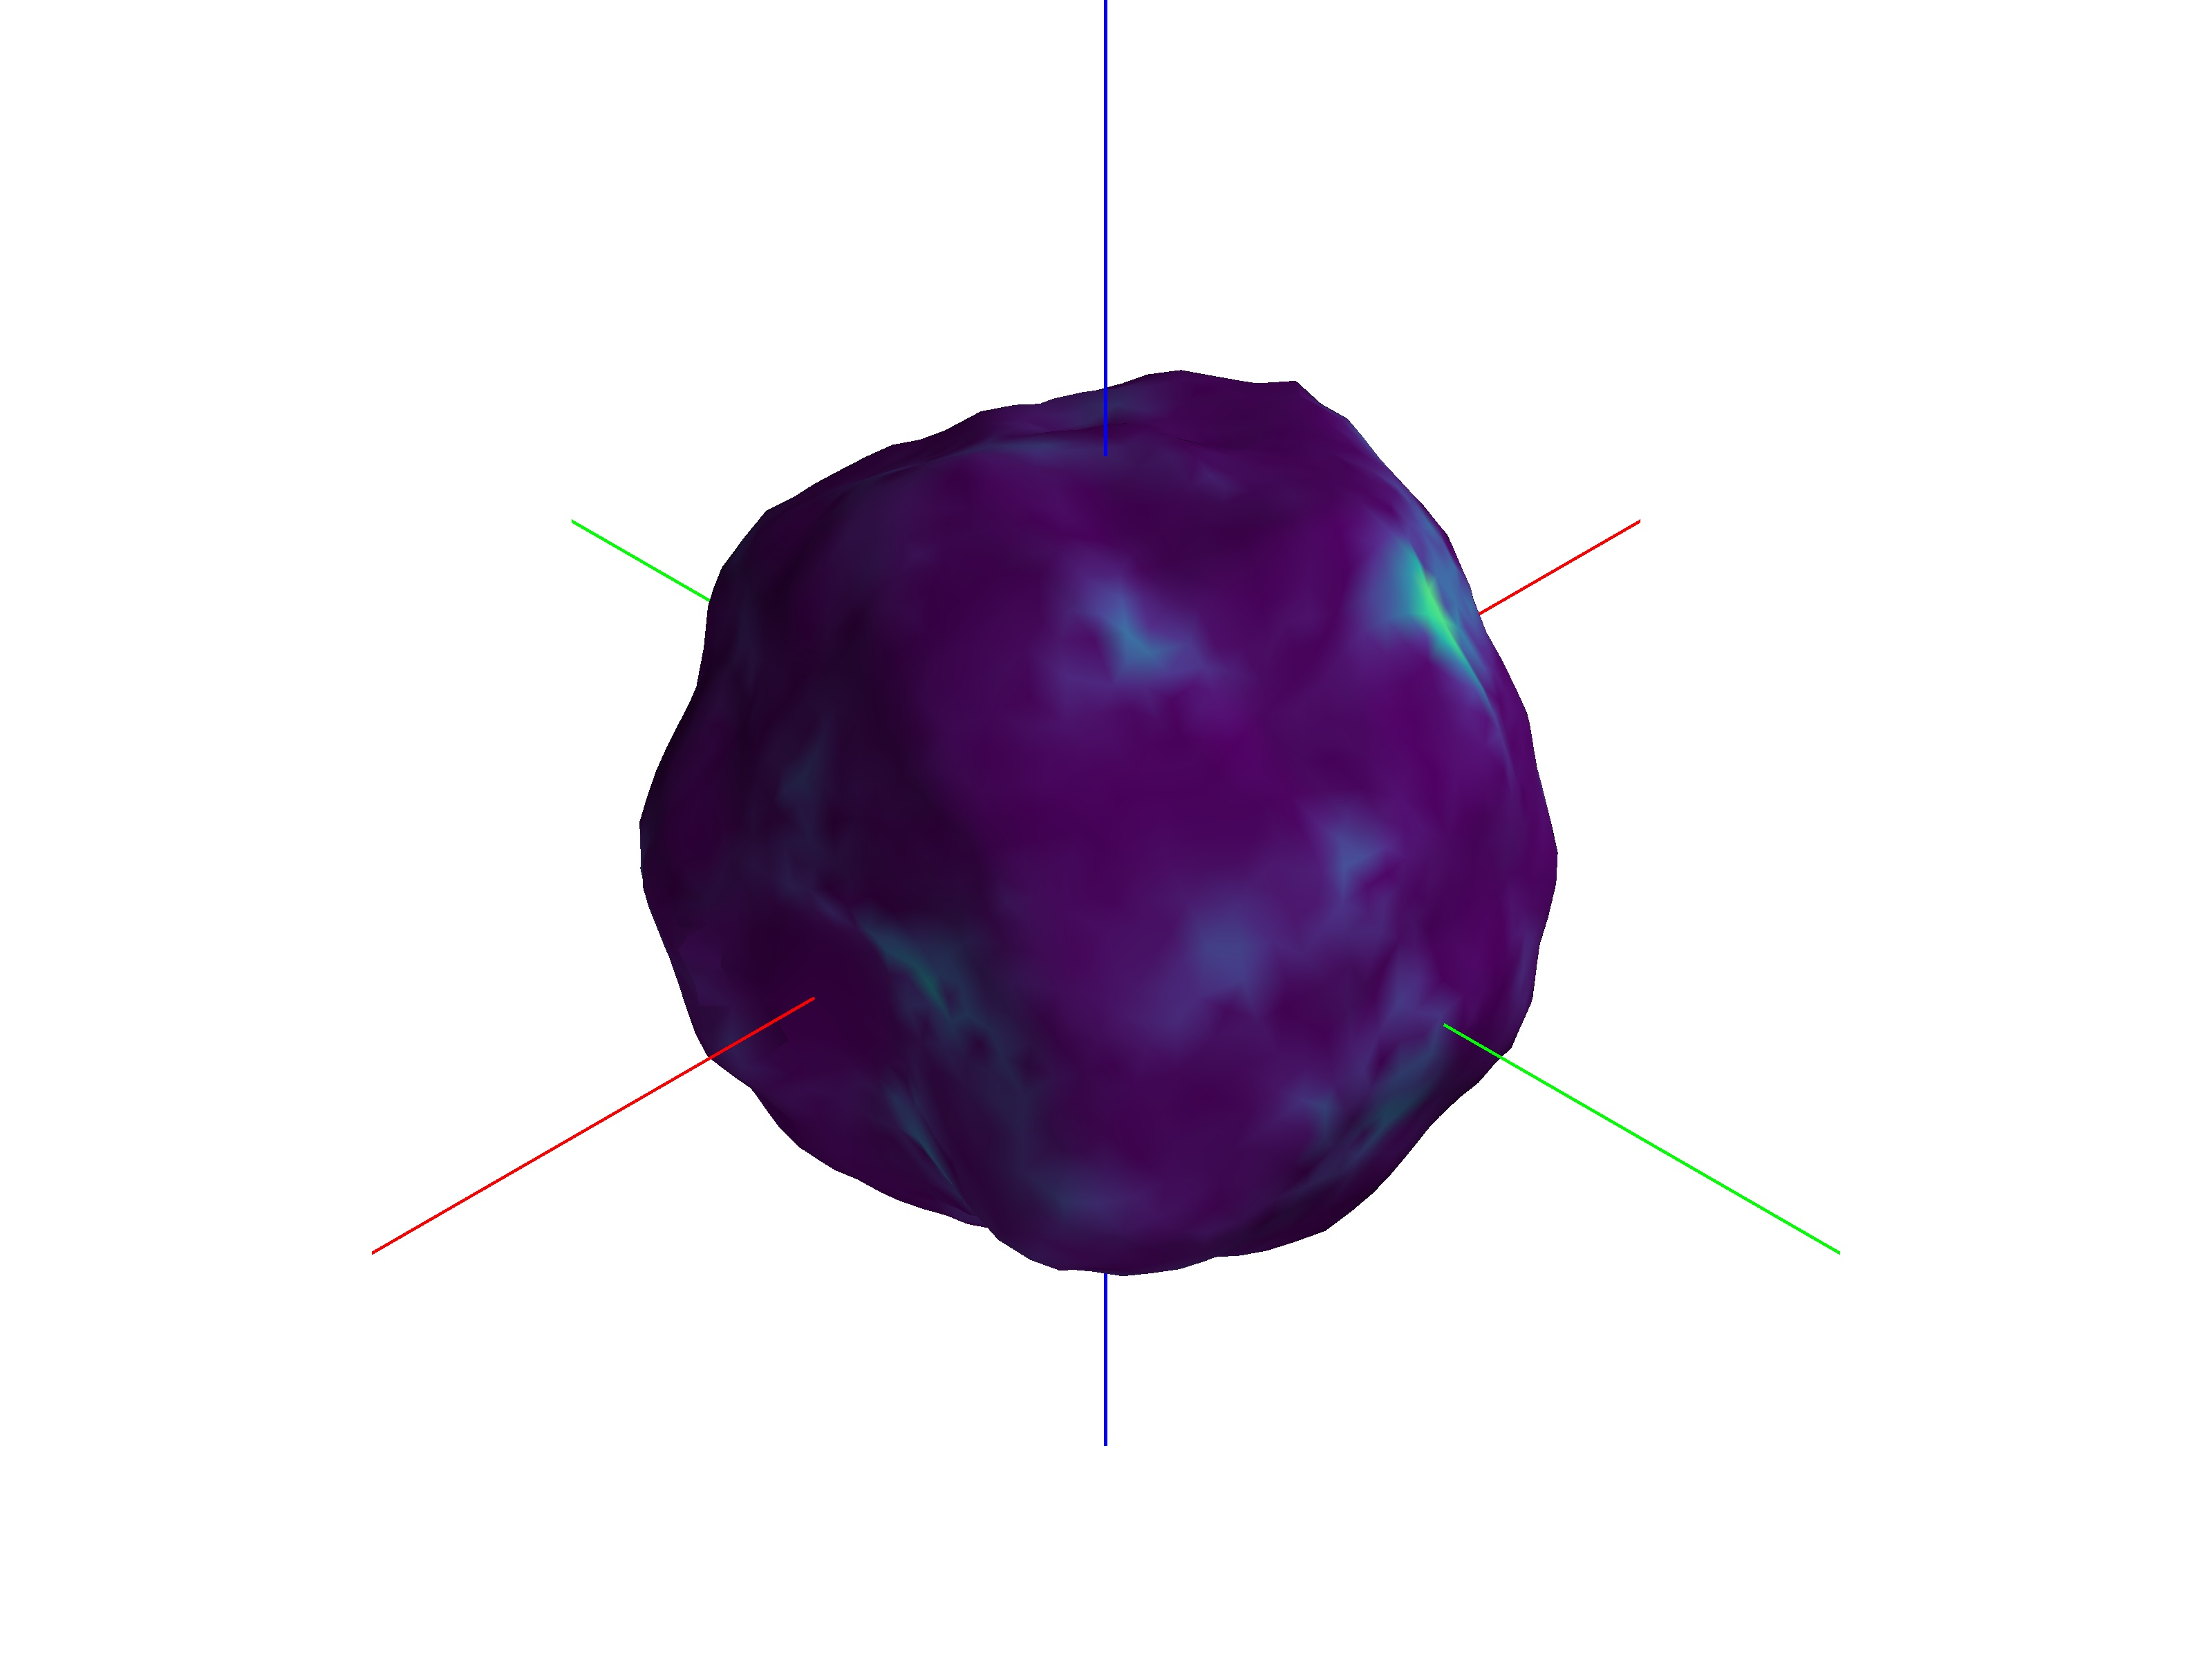
\includegraphics[trim={30cm 15cm 30cm 15cm},clip,height=0.25\textheight,width=0.5\textwidth,keepaspectratio]{figures/dynamic_exploration/52760/partial_weights_11249.jpg}}%

    \subcaptionbox{\SI{100}{\percent} of measurements\label{fig:52760_partial_weights_100}}{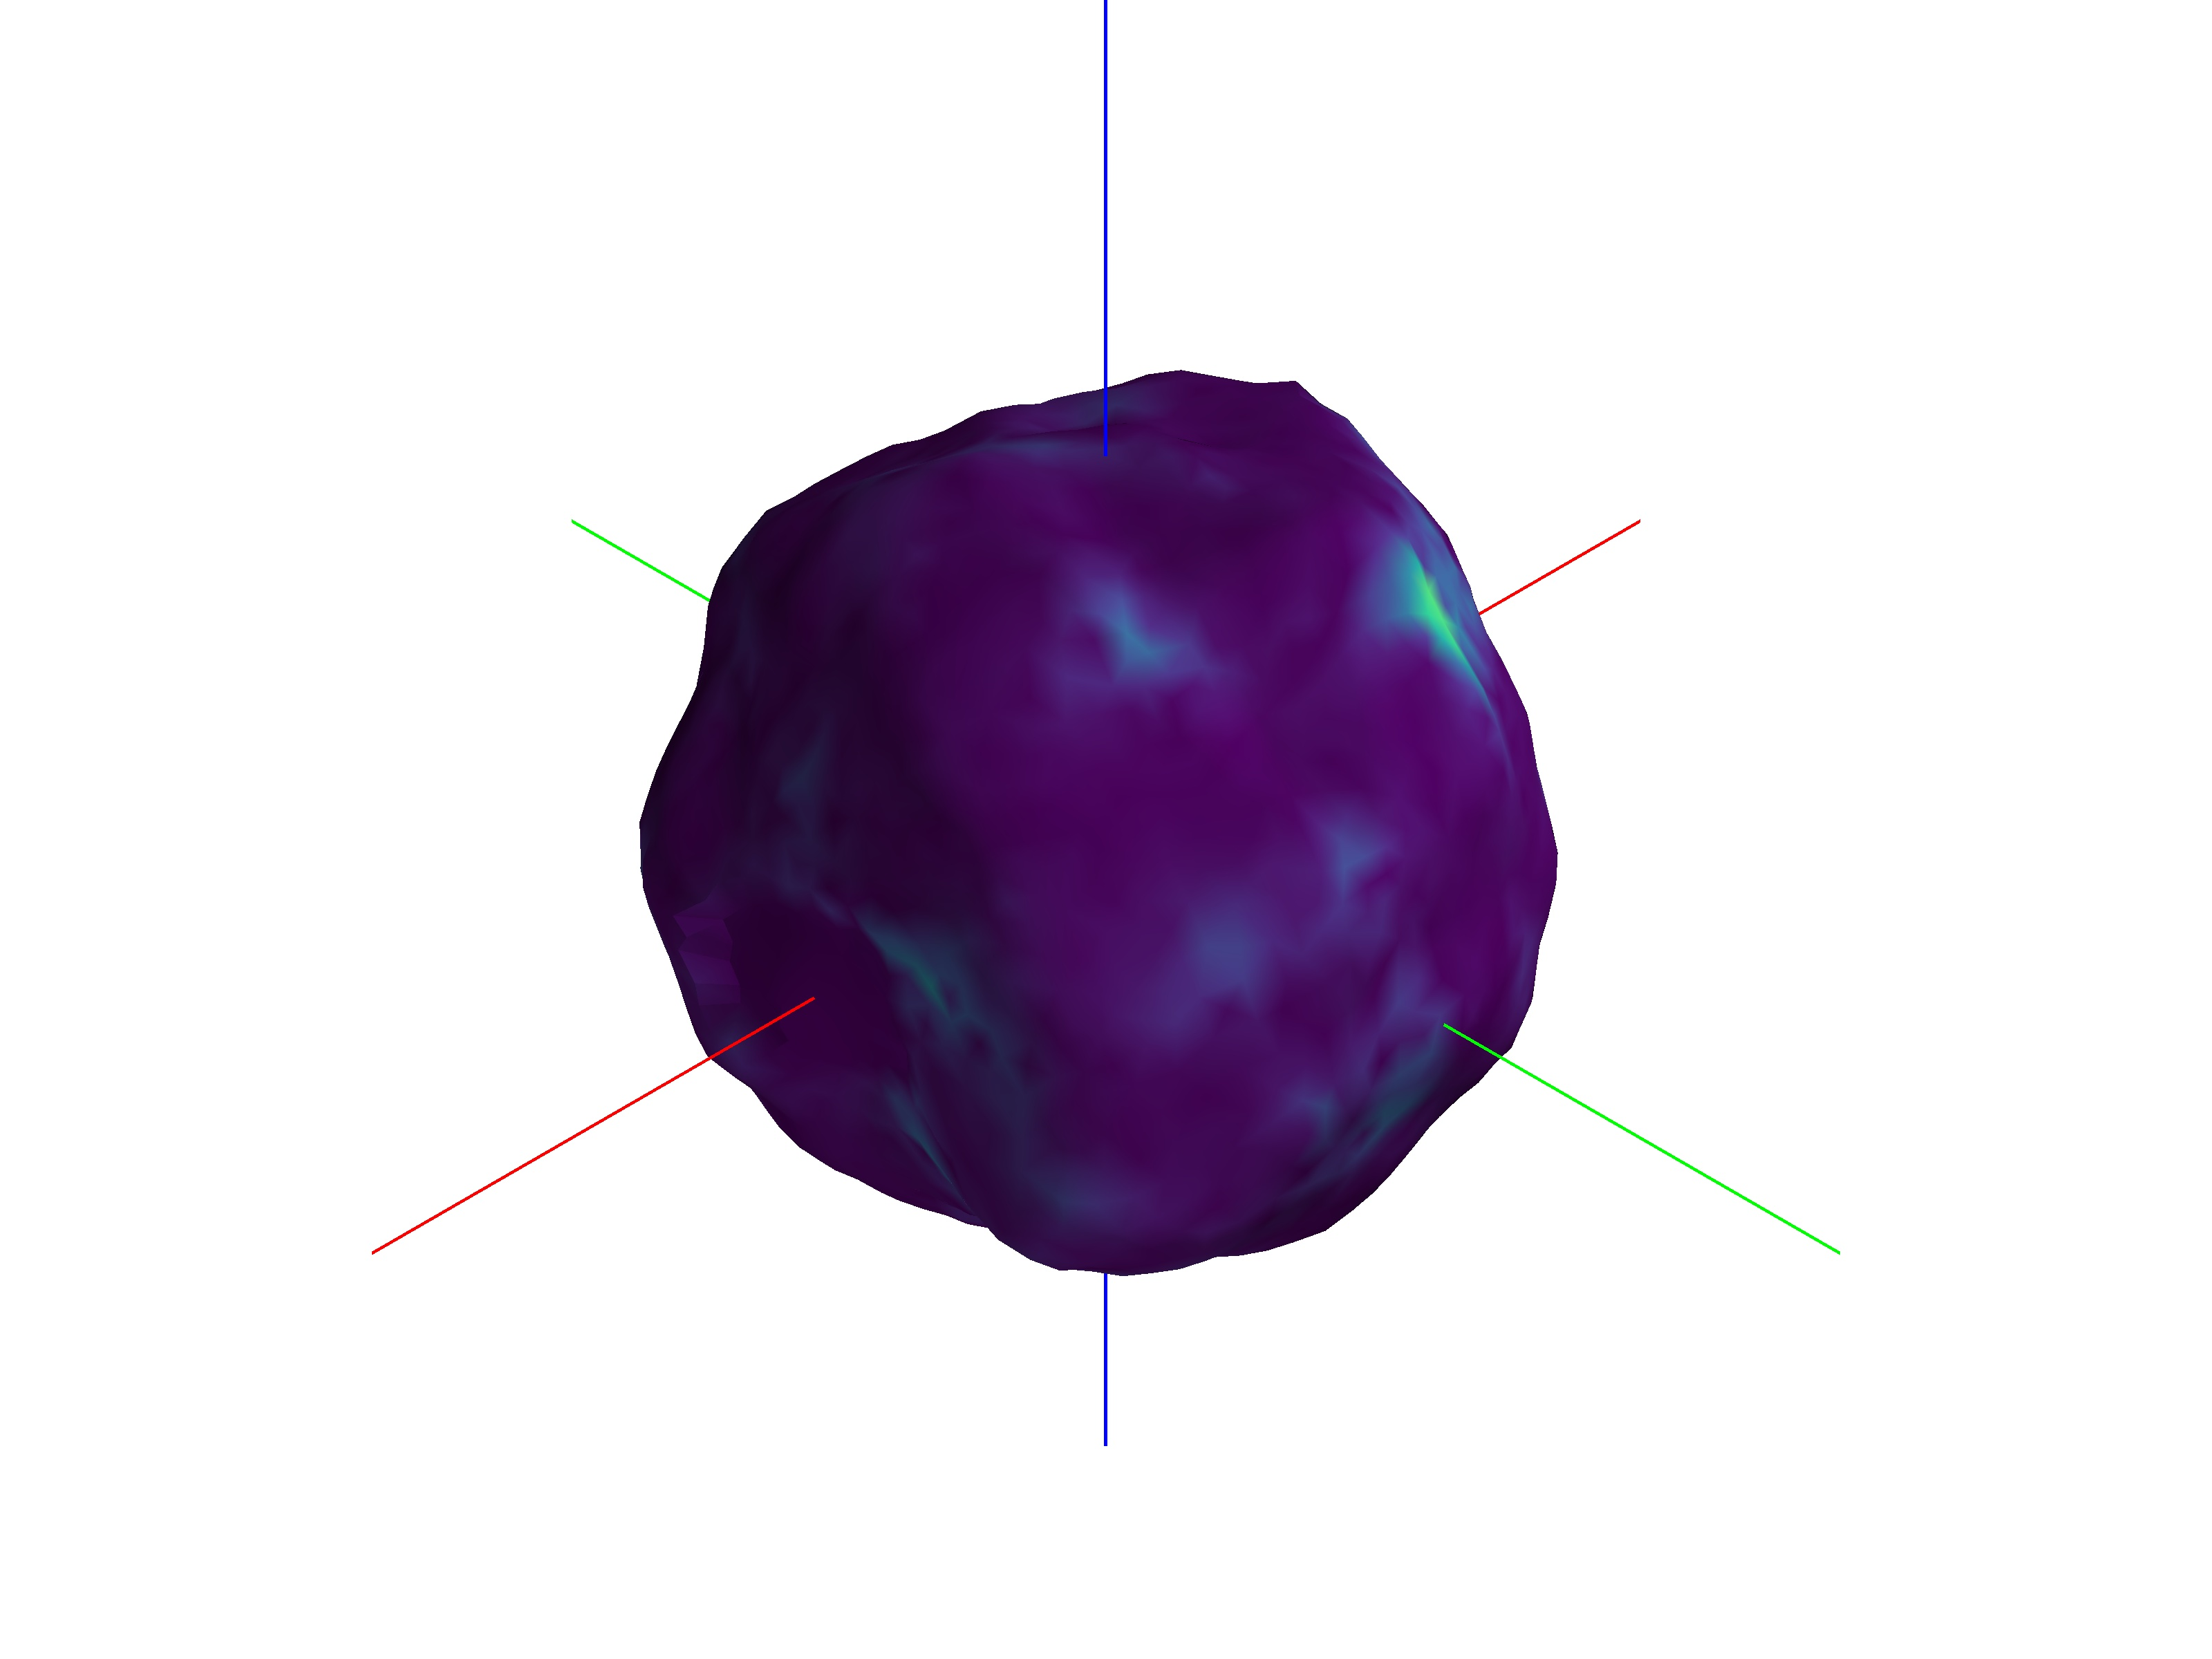
\includegraphics[trim={30cm 15cm 30cm 15cm},clip,height=0.25\textheight,width=0.5\textwidth,keepaspectratio]{figures/dynamic_exploration/52760/partial_weights_14998.jpg}}%
    \subcaptionbox{True Shape Model\label{fig:52760_weights_truth}}{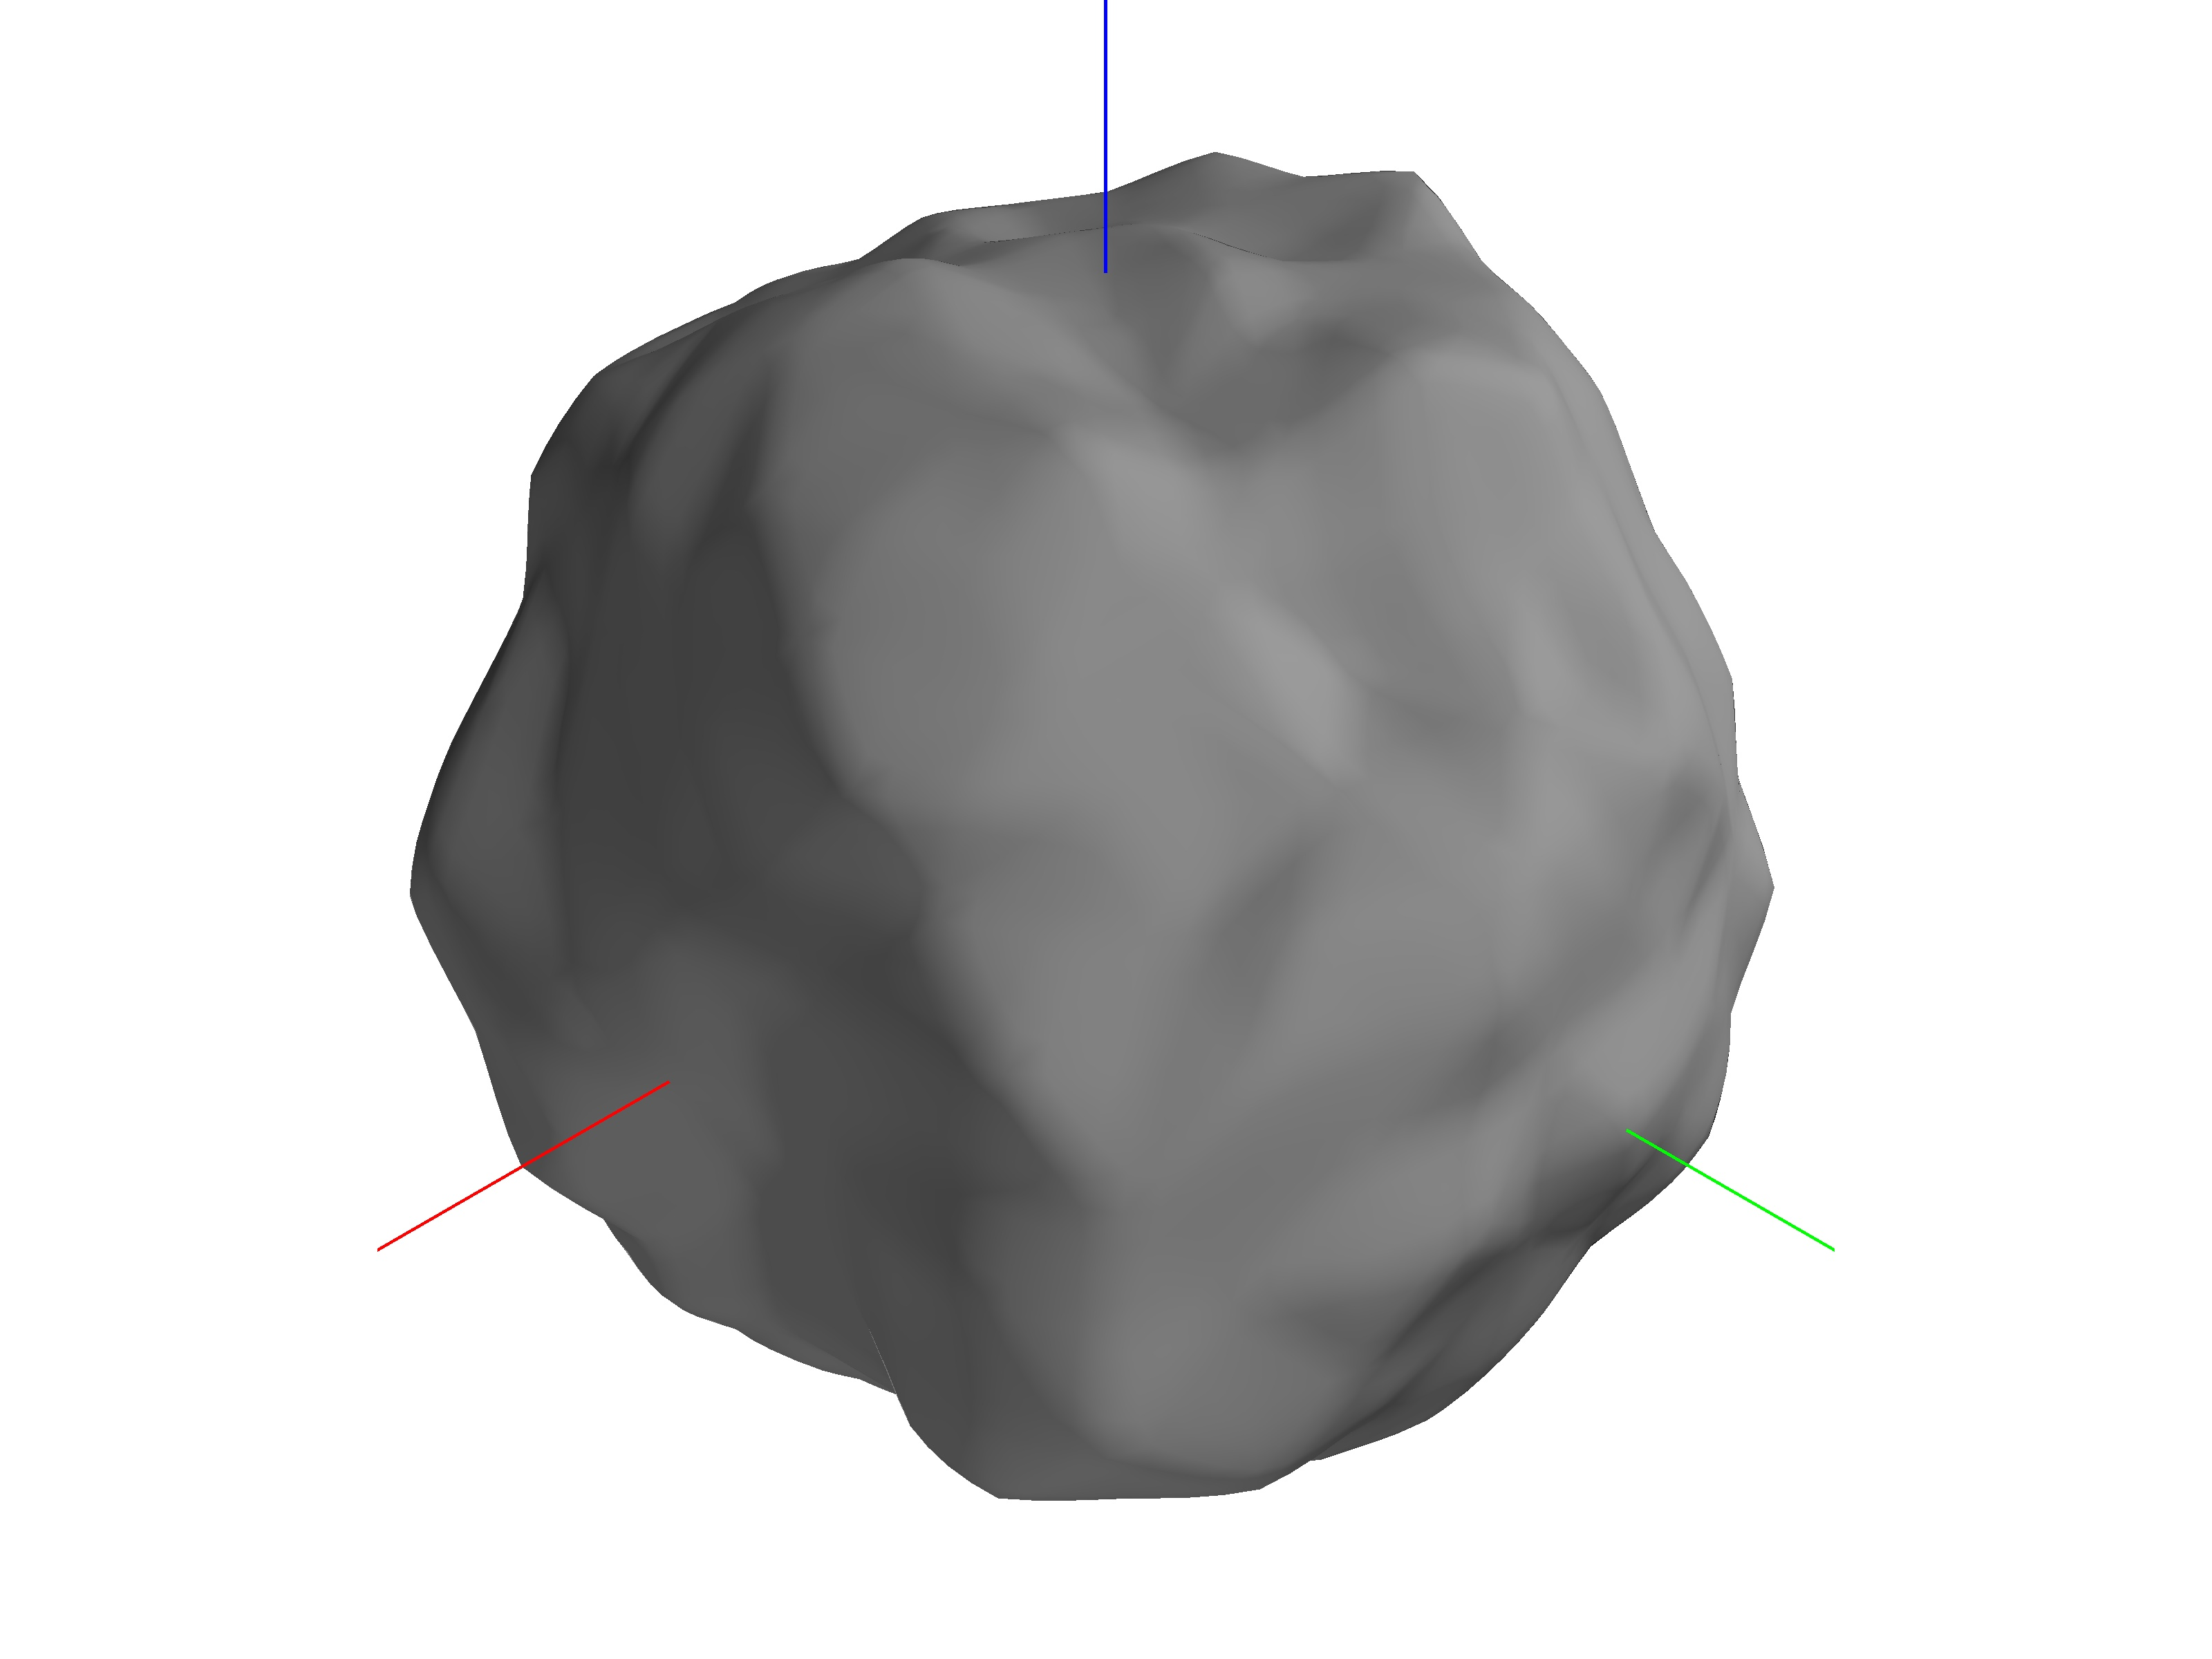
\includegraphics[trim={15cm 0cm 15cm 5cm},clip,height=0.25\textheight,width=0.5\textwidth,keepaspectratio]{figures/mesh_update/52760/truth.jpg}}
    \caption[Asteroid 52760 shape reconstruction with uncertainty]{Incremental reconstruction of asteroid 52760. The images colored according to the shape uncertainty. Areas of high uncertainty are in yellow while ares of low uncertainty are in purple.~\label{fig:52760_weights_reconstruction}}
\end{figure}

\paragraph{Asteroid 4769 Castalia Reconstruction}

Asteroid 4769 Castalia is a small near Earth asteroid of the Apollo group.
In addition, it is classified as a potentially hazardous object with a closed approach distance of less than \SI{0.05}{\astronomicalunit}.
Castalia was discovered in \num{1989} and is the first asteroid to be modeled using radar imagery~\cite{hudson1994}.
Castalia is composed of two distinct lobes suggesting that it is a contact binary of two smaller objects held together by their mutual gravity.
\Cref{fig:castalia_weights_reconstruction} show the shape reconstruction at several discrete points during the simulation.
In addition~\cref{fig:castalia_weights_reconstruction} displays the vertex uncertainty \( w_i \) as a colormap on the surface. 
Areas of high uncertainty are denoted in yellow while areas of low uncertainty are in purple/blue.
Within \SI{50}{\percent} of the simulation span the spacecraft is able to achieve an accurate estimate of the true shape of Castalia.

\begin{figure}[htbp]
    \centering
    \subcaptionbox{Initial Shape Estimate\label{fig:castalia_partial_weights_0}}{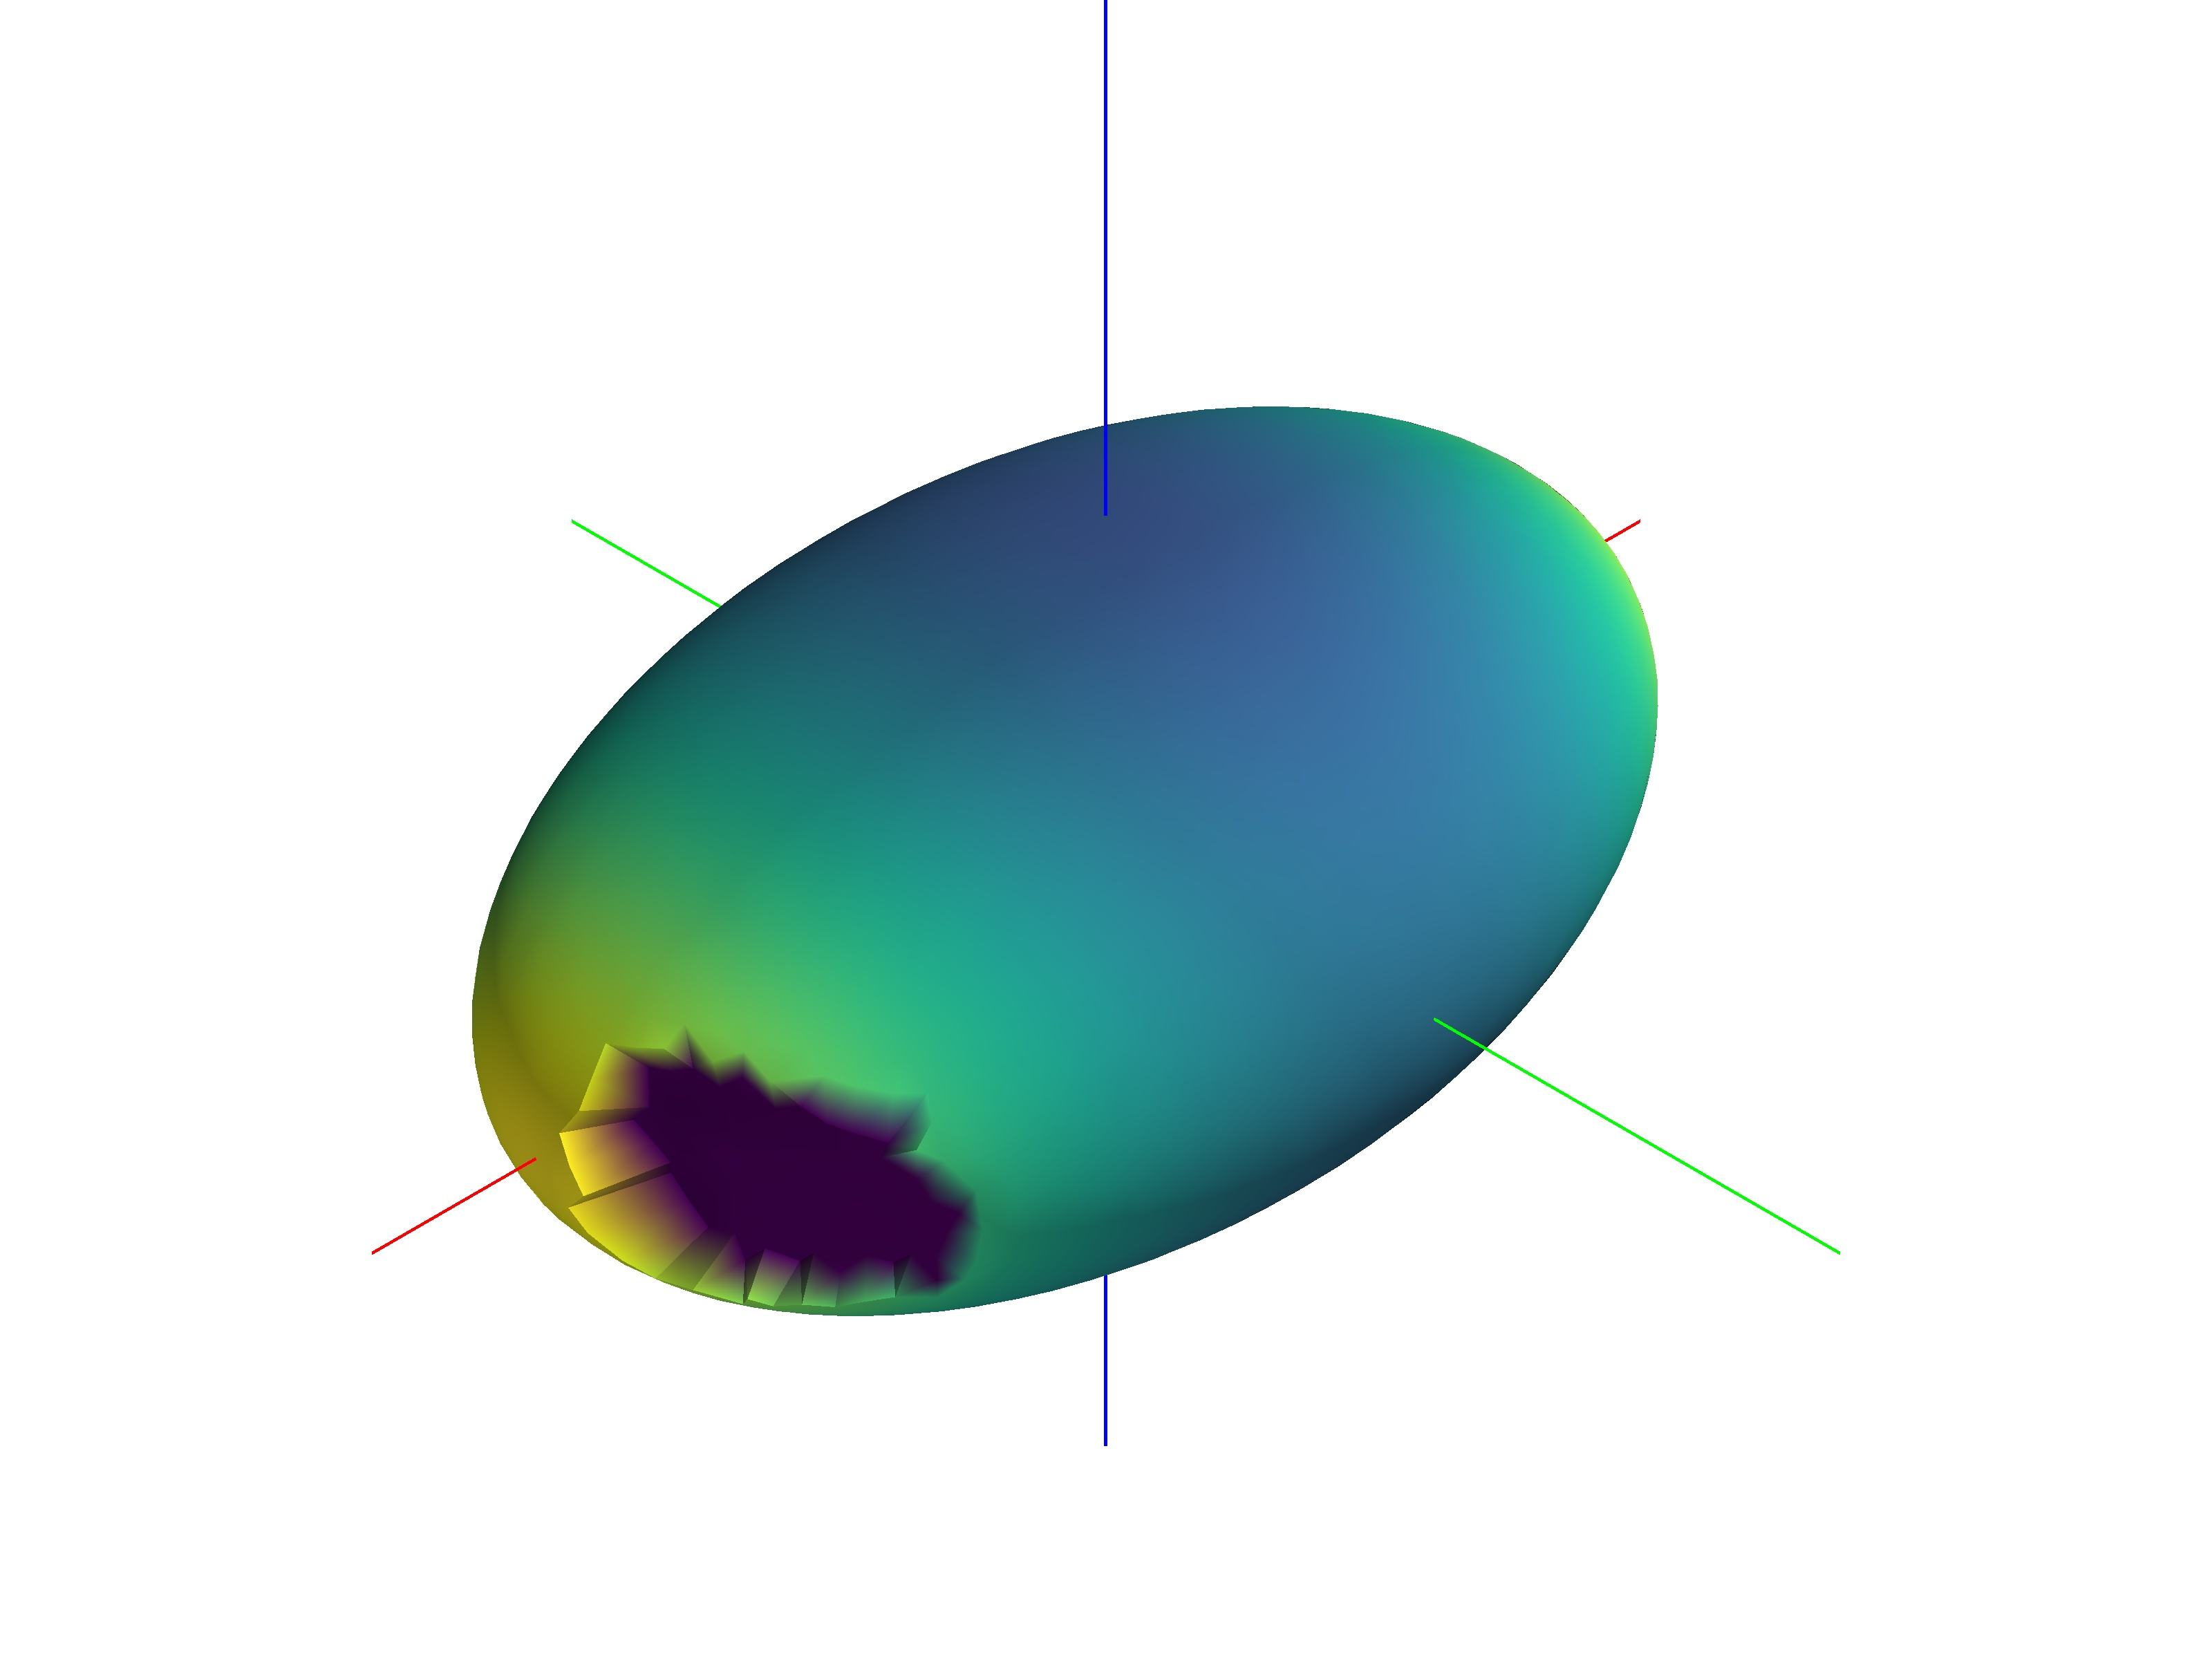
\includegraphics[trim={15cm 10cm 15cm 10cm},clip,height=0.5\textheight,width=0.3\textwidth,keepaspectratio]{figures/dynamic_exploration/castalia/partial_weights_1.jpg}}%
    \subcaptionbox{\SI{25}{\percent} of measurements added\label{fig:castalia_partial_weights_25}}{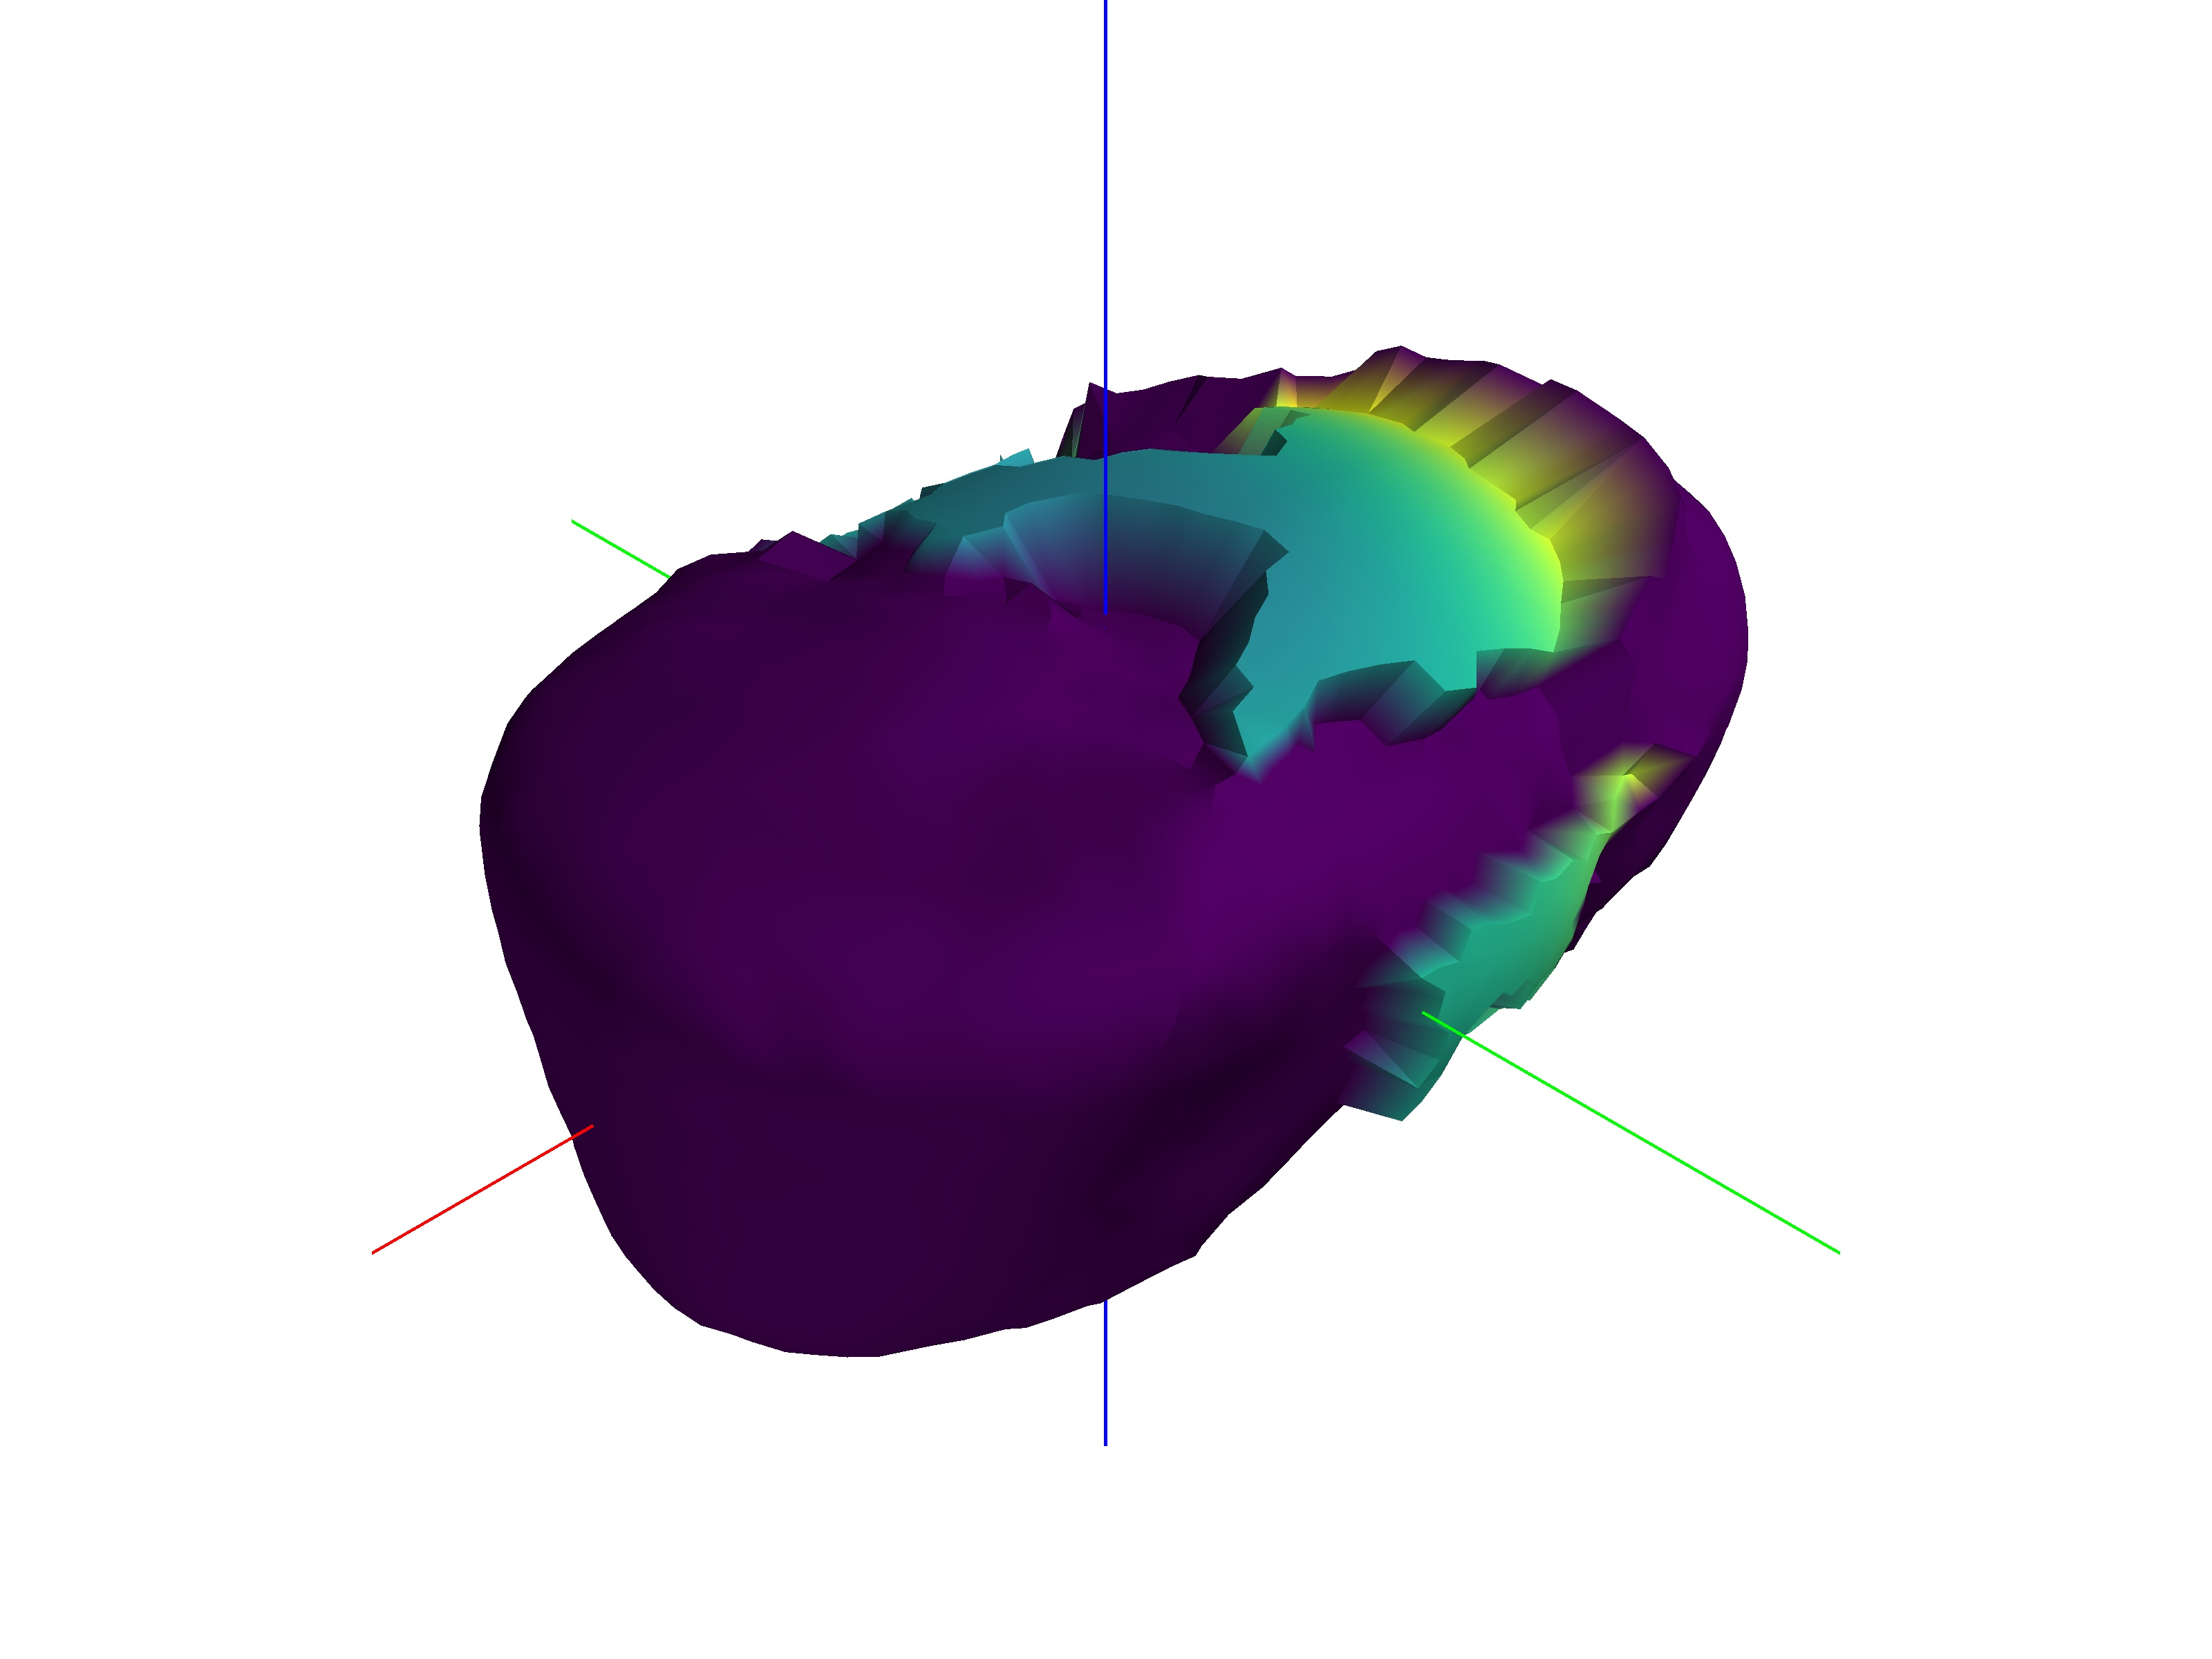
\includegraphics[trim={15cm 10cm 15cm 10cm},clip,height=0.5\textheight,width=0.3\textwidth,keepaspectratio]{figures/dynamic_exploration/castalia/partial_weights_3749.jpg}}%
    \subcaptionbox{\SI{50}{\percent} of measurements added\label{fig:castalia_partial_weights_50}}{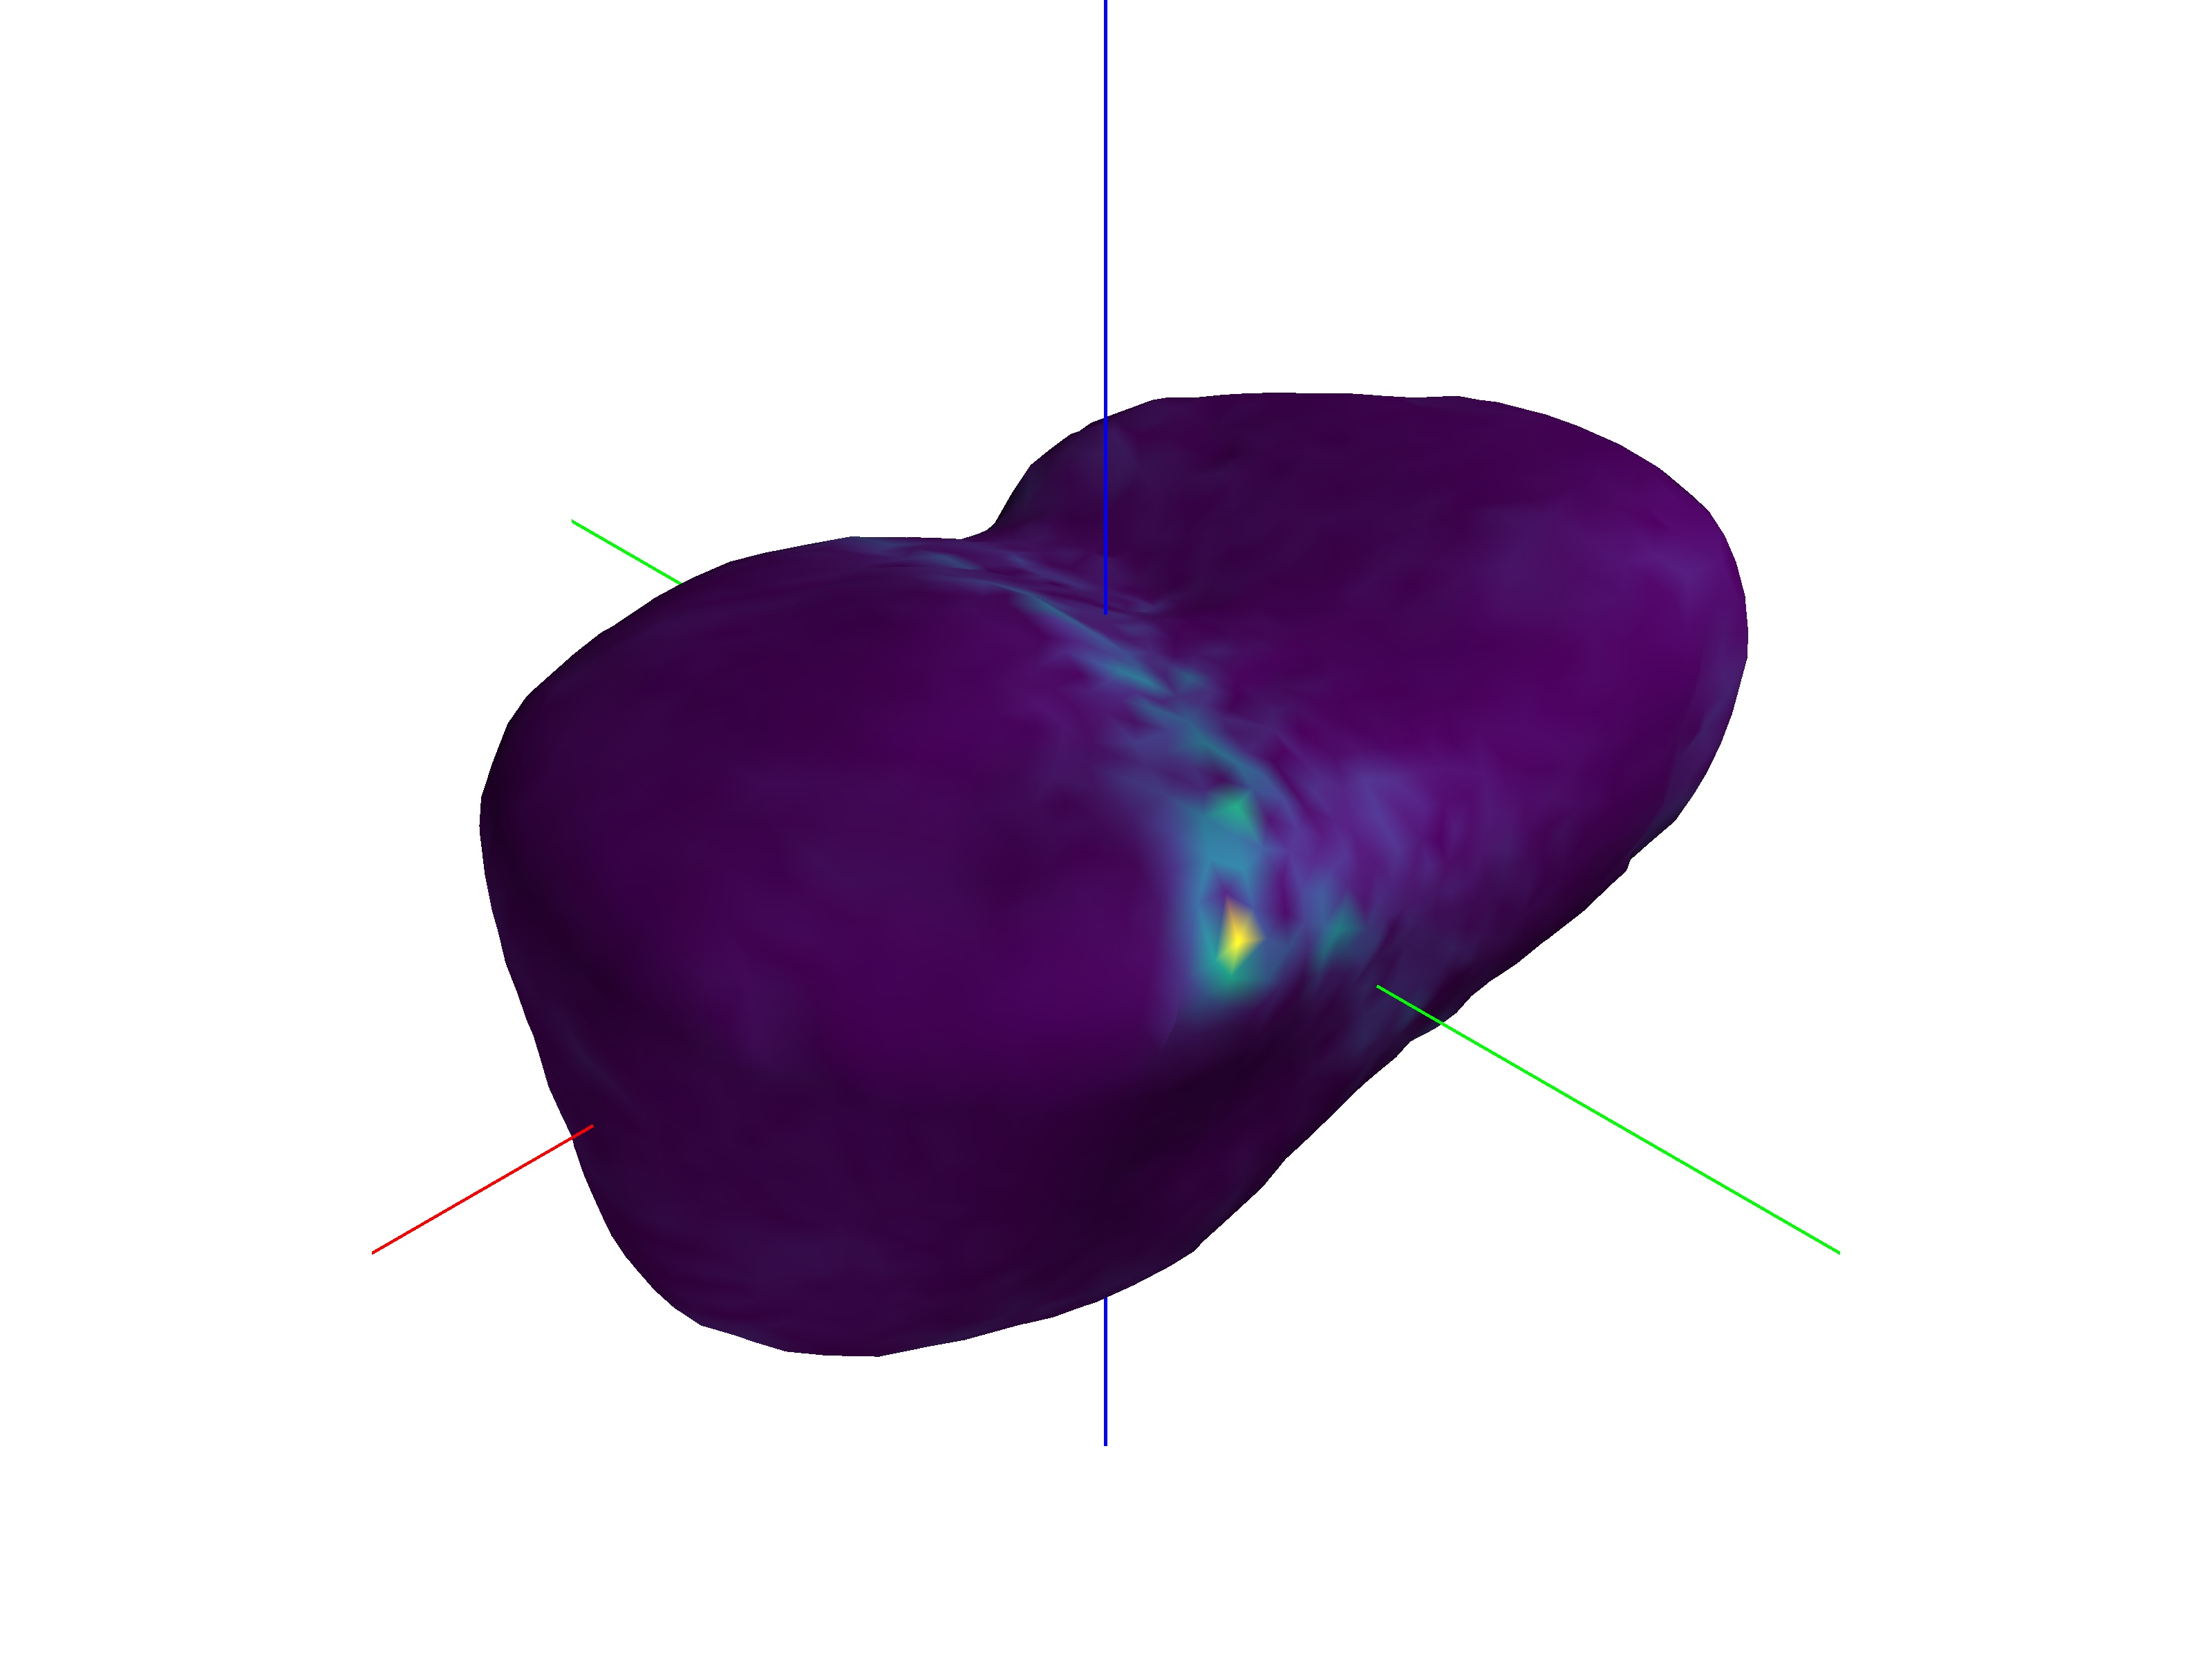
\includegraphics[trim={15cm 10cm 15cm 10cm},clip,height=0.5\textheight,width=0.3\textwidth,keepaspectratio]{figures/dynamic_exploration/castalia/partial_weights_7499.jpg}}

    \subcaptionbox{\SI{75}{\percent} of measurements added\label{fig:castalia_partial_weights_75}}{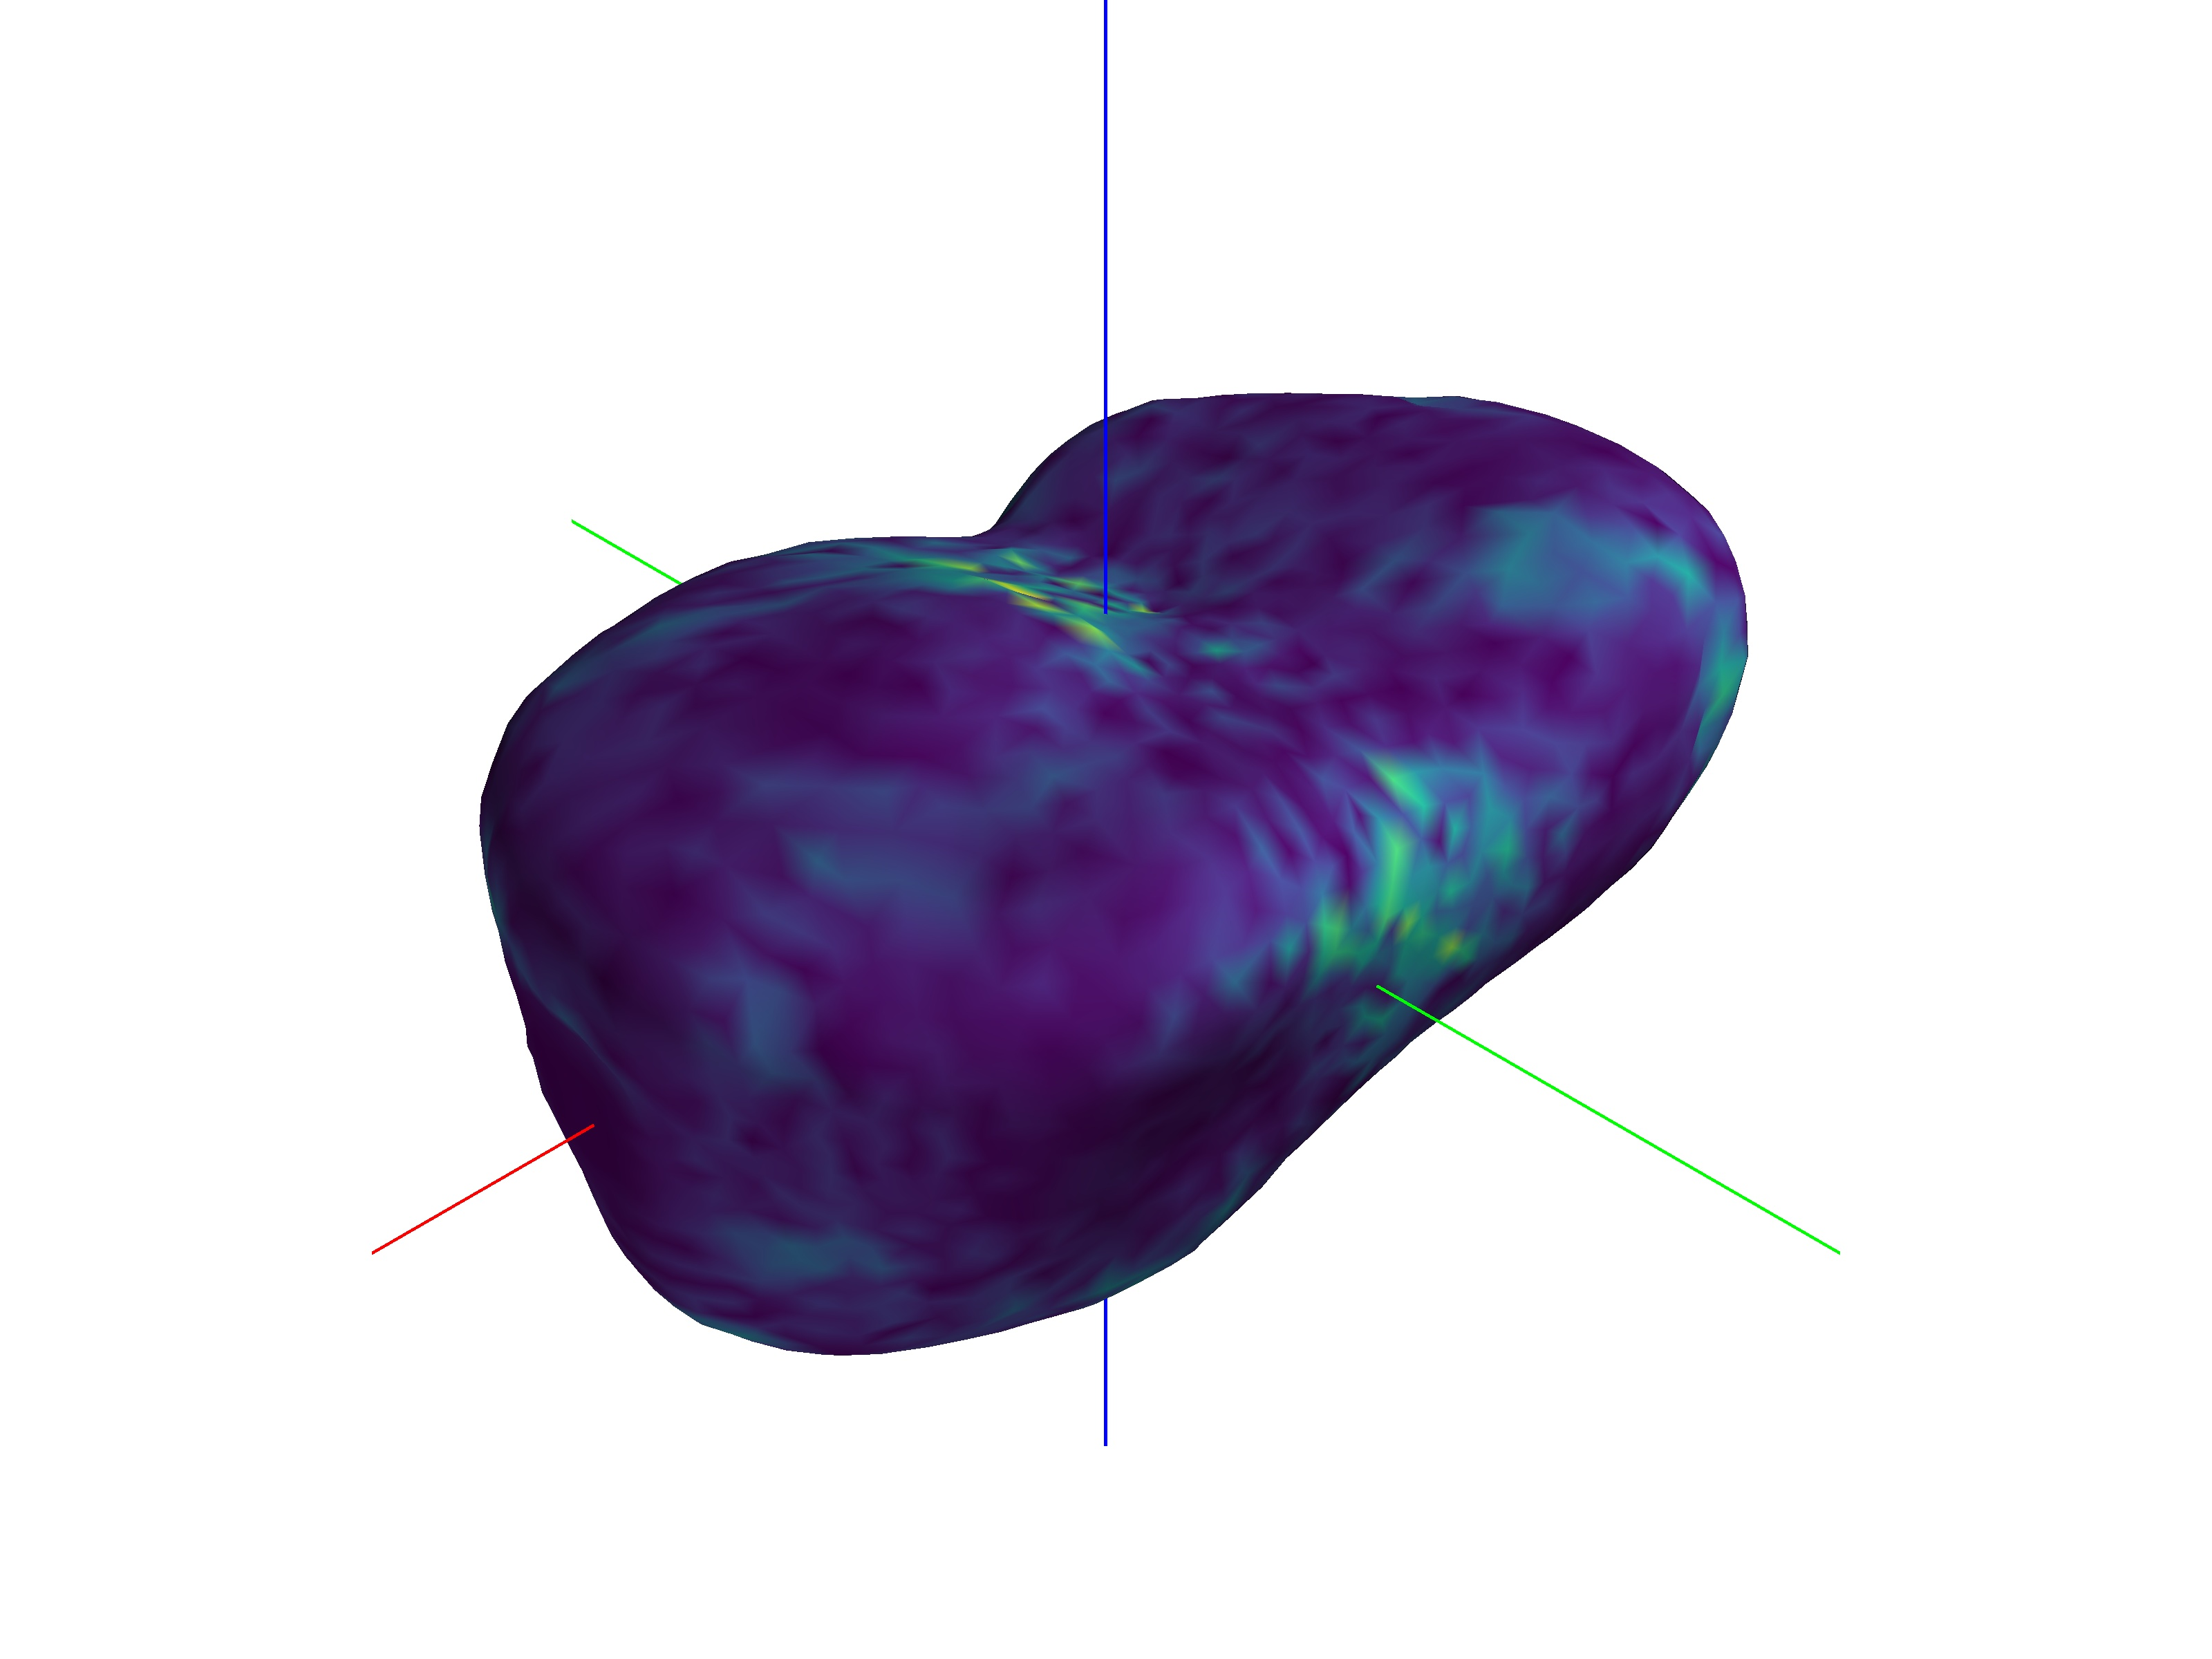
\includegraphics[trim={15cm 10cm 15cm 10cm},clip,height=0.5\textheight,width=0.3\textwidth,keepaspectratio]{figures/dynamic_exploration/castalia/partial_weights_11249.jpg}}%
    \subcaptionbox{\SI{100}{\percent} of measurements added\label{fig:castalia_partial_weights_100}}{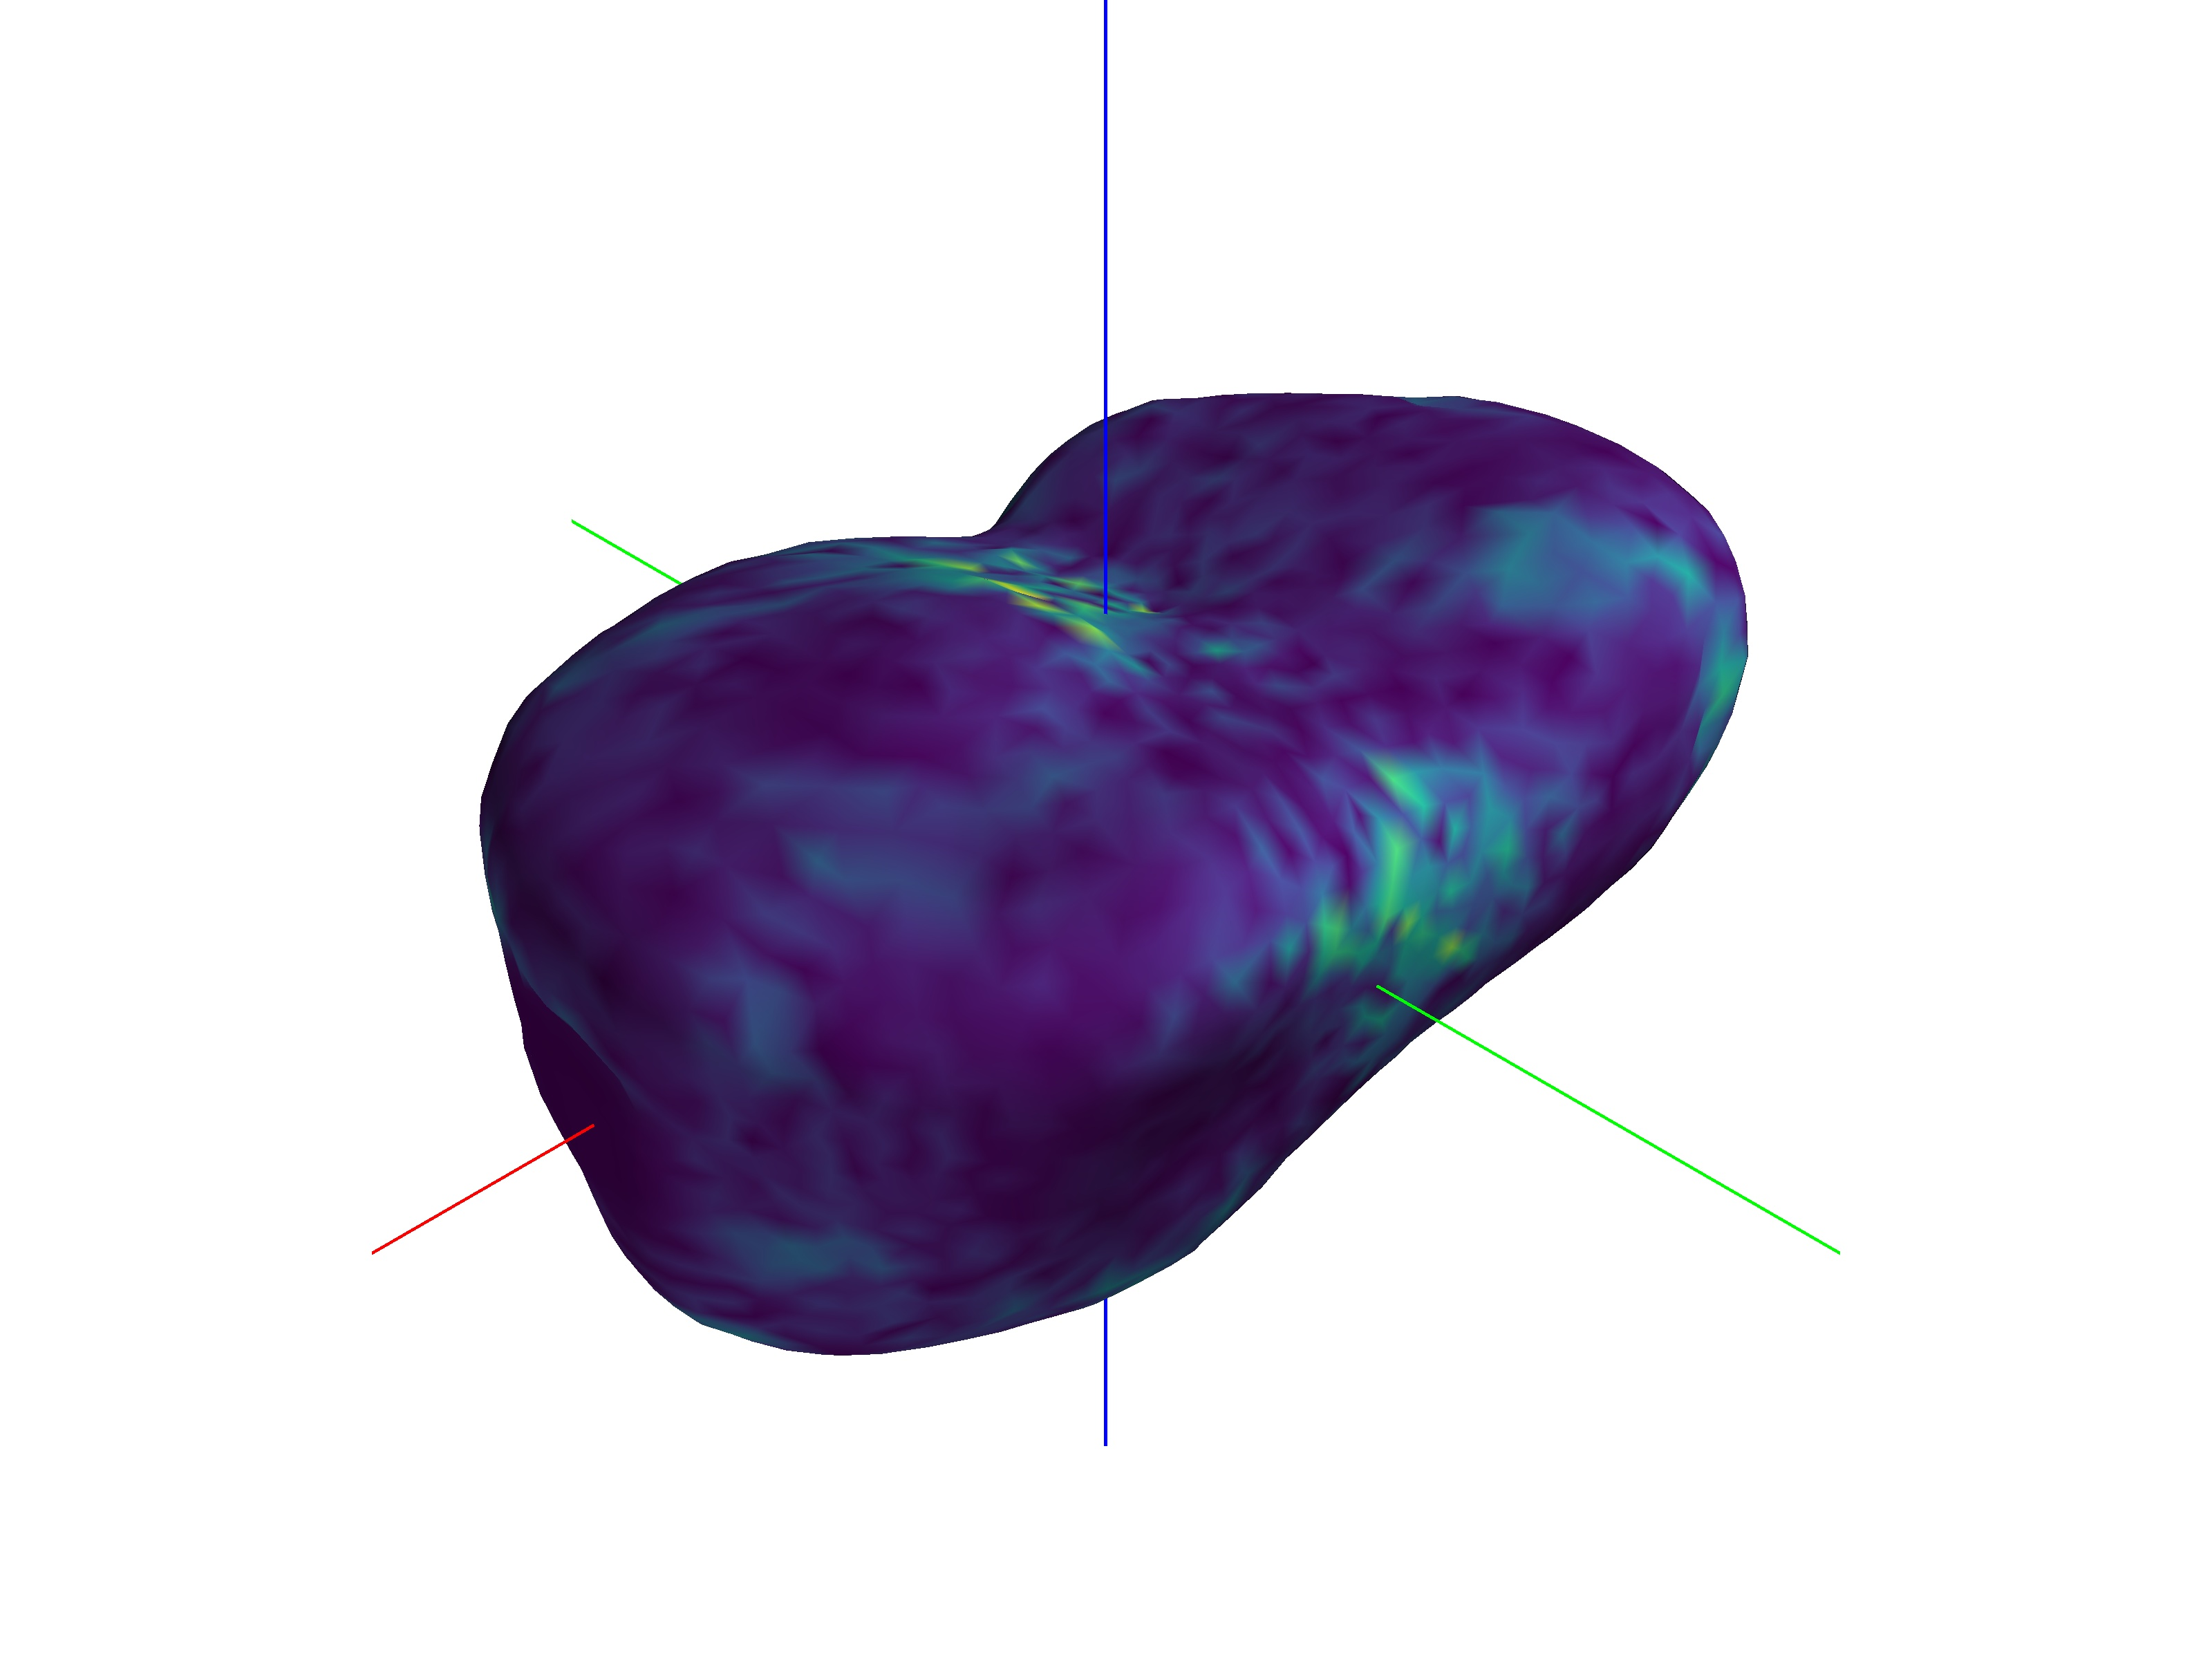
\includegraphics[trim={15cm 10cm 15cm 10cm},clip,height=0.5\textheight,width=0.3\textwidth,keepaspectratio]{figures/dynamic_exploration/castalia/partial_weights_14998.jpg}}%
    \subcaptionbox{True Shape Model\label{fig:castalia_weights_truth}}{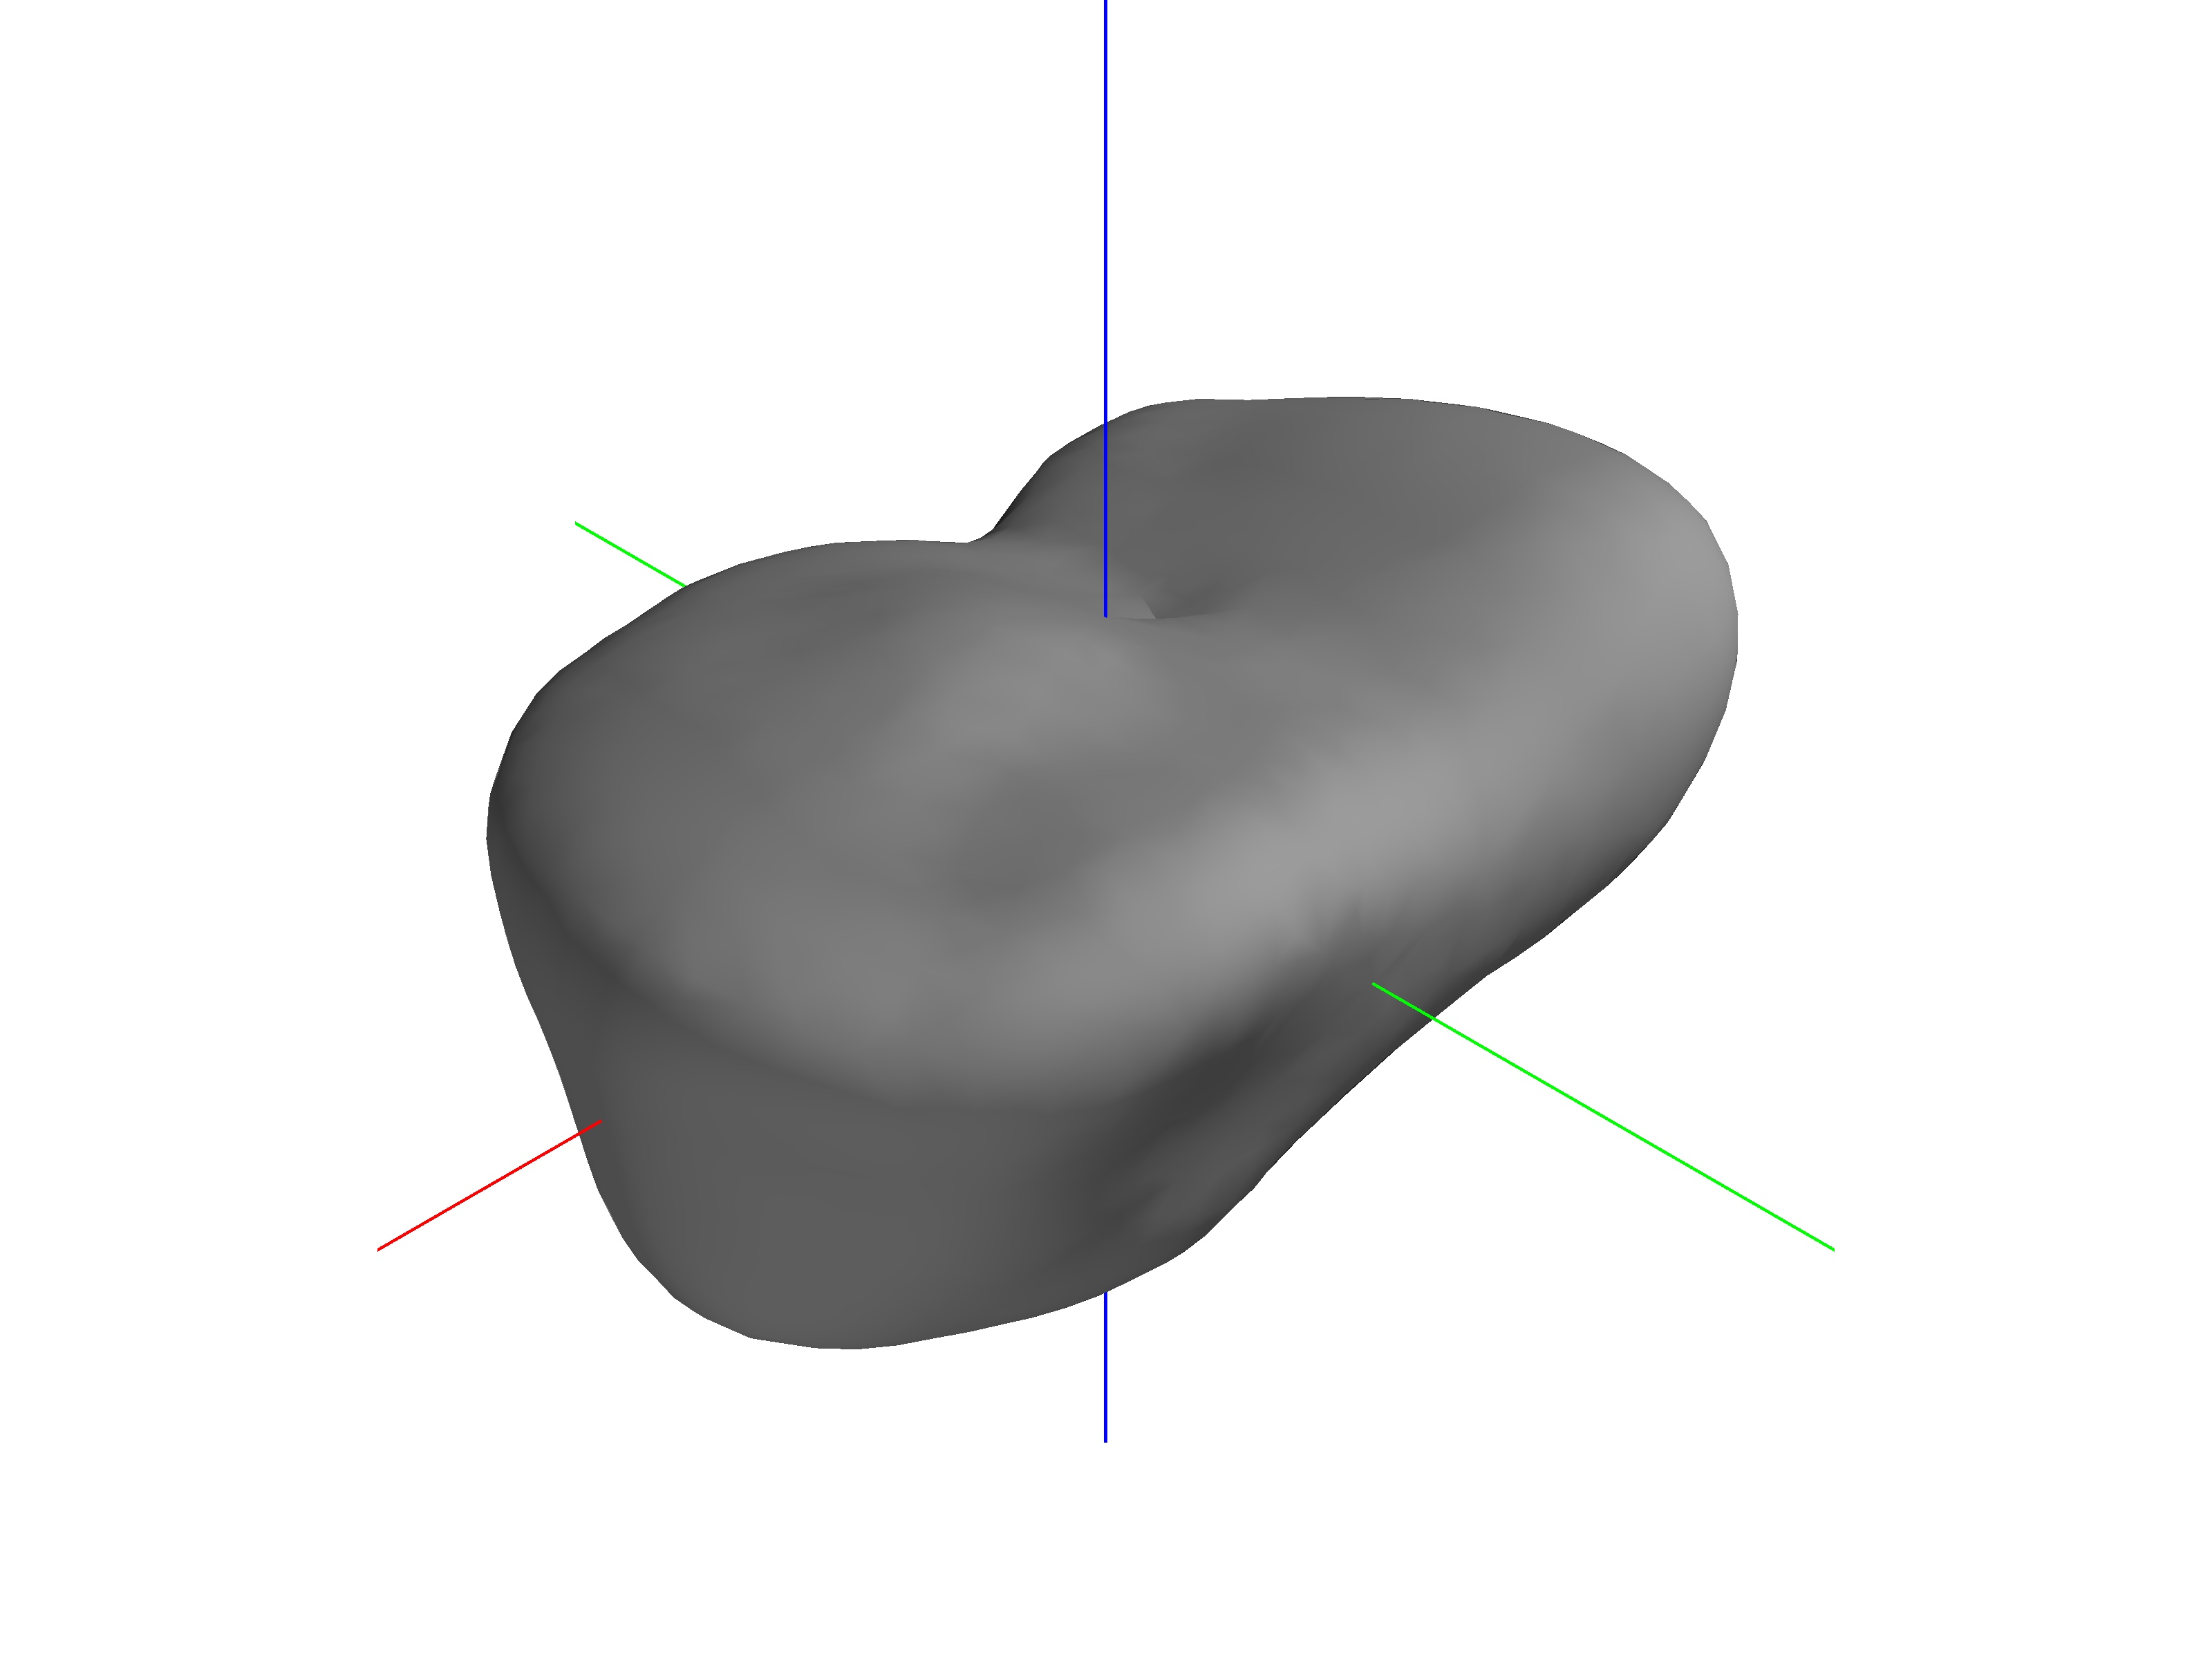
\includegraphics[trim={15cm 10cm 15cm 10cm},clip,height=0.5\textheight,width=0.3\textwidth,keepaspectratio]{figures/mesh_update/castalia/truth.jpg}}
    \caption[Asteroid Castalia shape reconstruction with uncertainty]{Incremental reconstruction of asteroid Castalia. The images colored according to the shape uncertainty. Areas of high uncertainty are in yellow while ares of low uncertainty are in purple.~\label{fig:castalia_weights_reconstruction}}
\end{figure}

\Cref{fig:castalia_metrics} shows the total normalized uncertainty and percent error for the volume estimate. 
The plots show that the reconstruction converges to an accurate shape estimate after approximately \SI{8000}{\second}.
In addition, the volume estimate is initially a much larger value but quickly converges to the true value.
\begin{figure}[htbp]
    \centering
    \tikzsetnextfilename{castalia_metrics}
\begin{tikzpicture}[baseline]
    \begin{groupplot}[
        group style={
            group name={castalia_metrics},
            group size=1 by 2,
            xlabels at=edge bottom,
            ylabels at=edge left,
            xticklabels at=edge bottom,
        },
        xlabel={Normalized Time},
        scale only axis,
        width=0.8\textwidth,
        height=0.1\textheight,
        ylabel style={align=center},
    ]
    \nextgroupplot[ylabel={Normalized\\Uncertainty}]
    \addplot [ultra thick, color=blue, mark=none] table [x=NORMALIZED_TIME, y=NORMALIZED_UNCERTAINTY, col sep=comma] {figures/dynamic_exploration/castalia/uncertainty.csv};
    \addplot [ultra thick,red, mark=none, dashed] coordinates {
        (0.0, 0.0) (1.0, 0.0) 
    };

    \nextgroupplot[ylabel={Volume Percent\\Error}]
    \addplot [ultra thick, blue, mark=none] table [x=NORMALIZED_TIME, y=VOLUME_PERCENT_ERROR, col sep=comma] {figures/dynamic_exploration/castalia/volume.csv};
        \addplot [ultra thick,red, mark=none, dashed] coordinates {
            (0.0, 0.0) (1.0, 0.0) 
        };
\end{groupplot}
\end{tikzpicture}


    \caption{Normalized uncertainty and volume percent error for Castalia\label{fig:castalia_metrics}}
\end{figure}
The spacecraft autonomously navigates around asteroid Castalia to best minimize the cost function in~\cref{eq:control_cost}.


\section{Multi-resolution Landing Area Refinement}\label{sec:landing_refinement}

In this section, we consider a scenario of autonomous landing on the surface of asteroid, once its shape is constructed as described above.
The shape reconstruction scheme is based on an initial coarse shape estimate that is iteratively updated with range measurements of the surface.
Consequently, the original mesh is uniformly distributed with a relatively large mesh size and many small topological features such as rocks or small craters may not be captured accurately.
However, these small features are critical for surface operations and safe landings.
In addition, it would be computationally prohibitive to have a uniformly high resolution mesh.
In this section, we extend the previous shape update approach to enable a much higher fidelity in a specific location.

\subsection{Landing Site Determination}

The selection of a landing site will typically require a vast quantity of data and weigh a multitude of possible metrics, such as scientific value, hardware constraints, timing and communication limits, or safety considerations. 
In our analysis we consider the surface slope, the distance to the surface, and a fictitious science metric in order to determine the best landing site based on the complete shape estimate.
This approach allows for a spacecraft to autonomously select and land on small body.

The surface slope is computed according to the method developed in Reference~\cite{scheeres1996}.
Due to the small size, and therefore low gravitational attraction, the force at each point on the surface is a combination of the gravitational attraction and the centripetal acceleration.
At the center of each face, \( f_i = \begin{bmatrix} f_x & f_y & f_z \end{bmatrix} \), we compute a modified surface acceleration as
\begin{align}\label{eq:surface_force}
    U_m = \omega^2 \begin{bmatrix} f_x \\ f_y \\ 0 \end{bmatrix} + \begin{bmatrix} U_x \\ U_y \\ U_z \end{bmatrix},
\end{align}
where \( \omega \in \R^1 \) is the angular velocity of the asteroid and \( U_i \) is computed from~\cref{eq:attraction}.
Then the surface slope can be computed from
\begin{align}\label{eq:surface_slope}
    \cos \parenth{ \pi - \phi } = \frac{\vc{n}_f \cdot U_m}{\norm{U_m}},
\end{align}
where \( \phi \in \R^1 \) is the surface slope defines the angle between the surface normal \( \vc{n}_f \in \R^3 \) and the force vector at the surface.
If \( \phi = \SI{0}{\degree} \) then the force vector and the surface normal are anti-parallel, while \( \phi > \SI{90}{\degree} \) means that a particle on the surface would be thrown off the body as the centripetal force is larger than the gravitational attraction.

Additionally, we compute the distance, using~\cref{eq:geodesic_distance}, between the spacecraft state and each face of the asteroid. 
Finally, we also assign a random science value to the surface in the form of a two dimensional Gaussian.
This can be modified depending on the specific objective of the mission. 

Utilizing these metric, a landing site is chosen to minimize the surface cost given as
\begin{align}\label{eq:surface_cost}
    J_l =  J_{\text{distance}} - J_{\text{science}},
\end{align}
subject to a hard inequality constraint requiring that the surface slope is less than a threshold, i.e., \( \phi \leq \phi_m \).

\todo{rewrite the above equation as a function of a candidate landing site location; we also need to describe how many points are considered for minimization; is it just the set of vertices}

\subsection{High-Resolution Mapping}\label{sec:refinement}

Mixed resolution surface meshes are routinely used in finite element and geometric modeling applications~\cite{botsch2010}.
As shown in Reference~\citenum{mcmahon2017}, utilizing mixed resolution shape models for asteroid missions offers the potential of reduced computational demands.
The computational cost of the polyhedron potential model, given by~\cref{eq:potential}, is roughly proportional to the number of faces in the shape model.
As a result, a uniformly high resolution shape would quickly become intractable for real time operations.
However, utilizing a mixed resolution approach allows for a high fidelity in a smaller mission critical area, such as a landing site, with a limited impact on the computational cost.

Once a suitable landing site is selected, the surrounding area is isolated and refined by adding new vertices and faces in the specified area.
The goal of refinement, or more generally remeshing, is given a mesh ( or a portion of it), compute another mesh whose elements satisfy some quality metrics while suitably approximating the original mesh.
In this work, we utilize the isotropic remeshing algorithm implemented in the Computational Geometry and Algorithms Library (CGAL).
\todo{add reference to CGAL}
This algorithm uses an iterative method which repeatedly splits long edges, collapses short edges, and relocates vertices until all edges are approximately the desired target edge length.
% TODO Think about adding PMP 6.12 image here

For example,~\cref{fig:cube_remesh} shows the isotropic remeshing result for the selected faces of a unit cube.
The original unit cube is composed of \num{8} vertices and \num{12} faces.
The two triangular faces of the visible side of the cube are selected for the isotropic remeshing operation as shown in~\cref{fig:cube_original_mesh}.
A target edge length of \num{0.1} is selected for these faces and used to generate~\cref{fig:cube_refine_mesh}.
The two large triangular faces are divided into a number of smaller triangular faces.
Furthermore, the additional faces are all approximately the same size and preserve the original surface of the cube.
After the isotropic remeshing operation the number of vertices has increased from \num{8} to \num{140}.
\begin{figure}[htbp]
    \centering
    \subcaptionbox{Original Cube\label{fig:cube_original_mesh}}{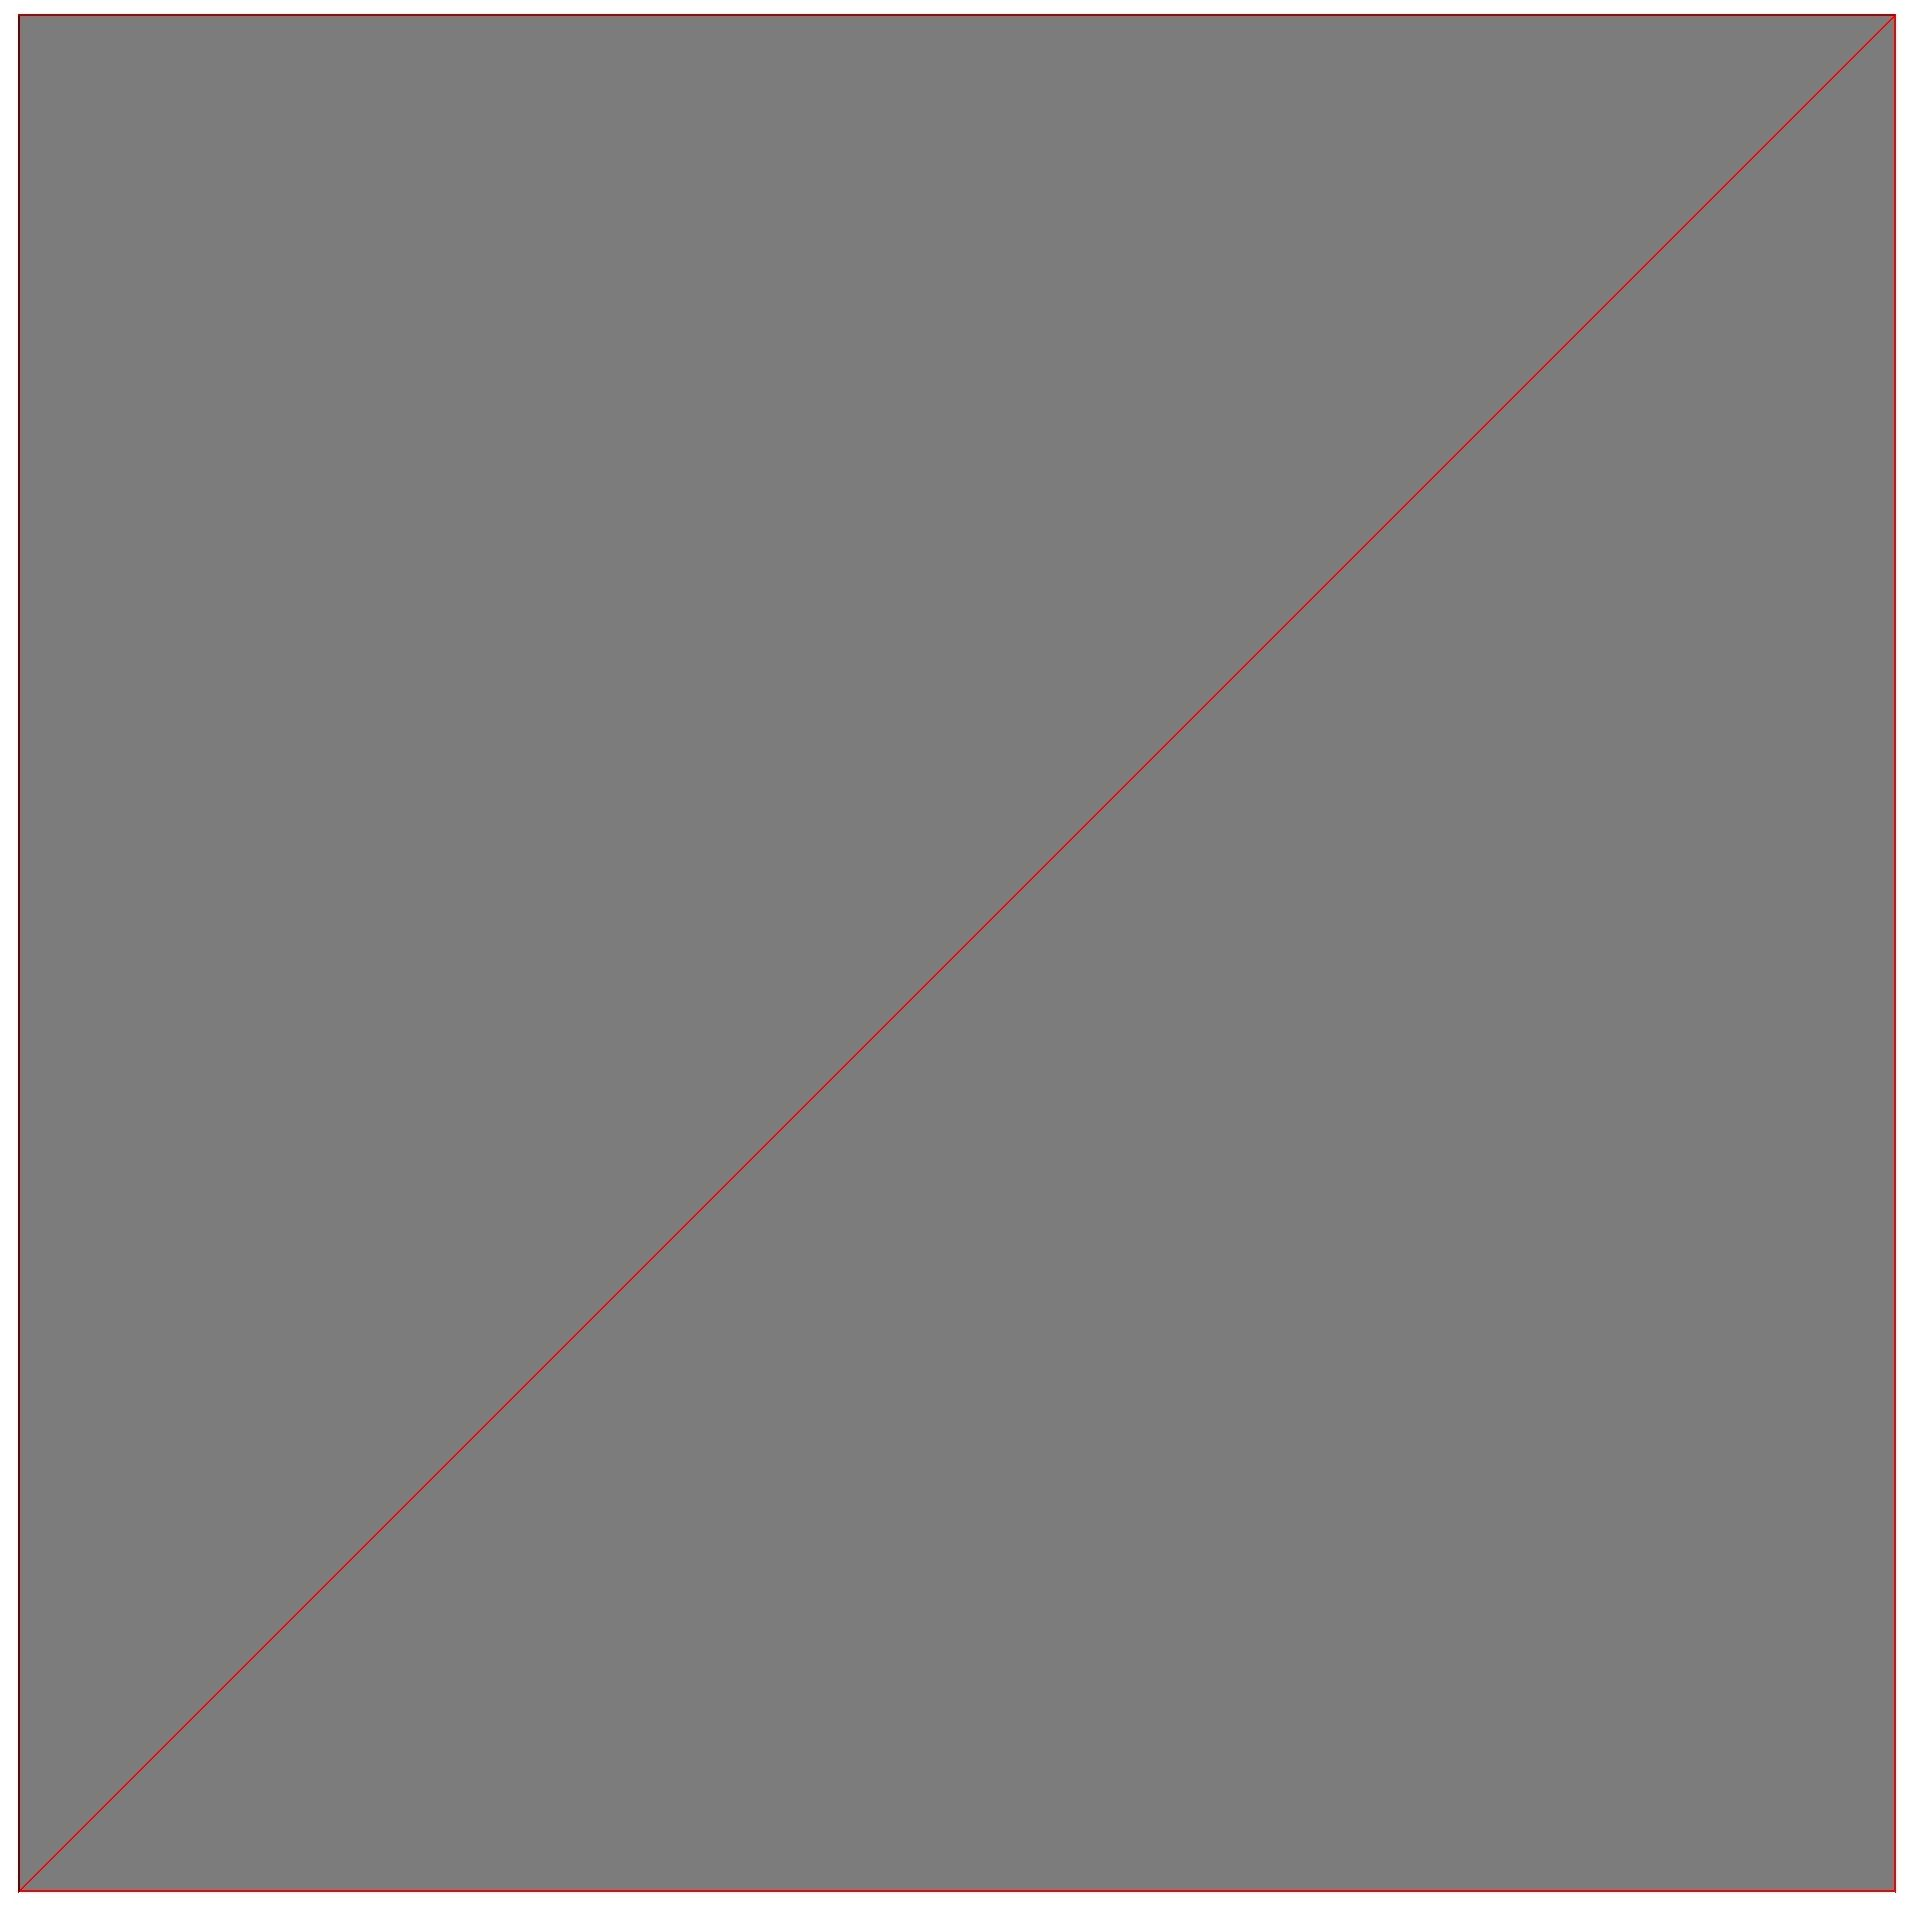
\includegraphics[width=0.45\textwidth]{figures/original_cube.jpg}}~
    \subcaptionbox{Remeshed Cube\label{fig:cube_refine_mesh}}{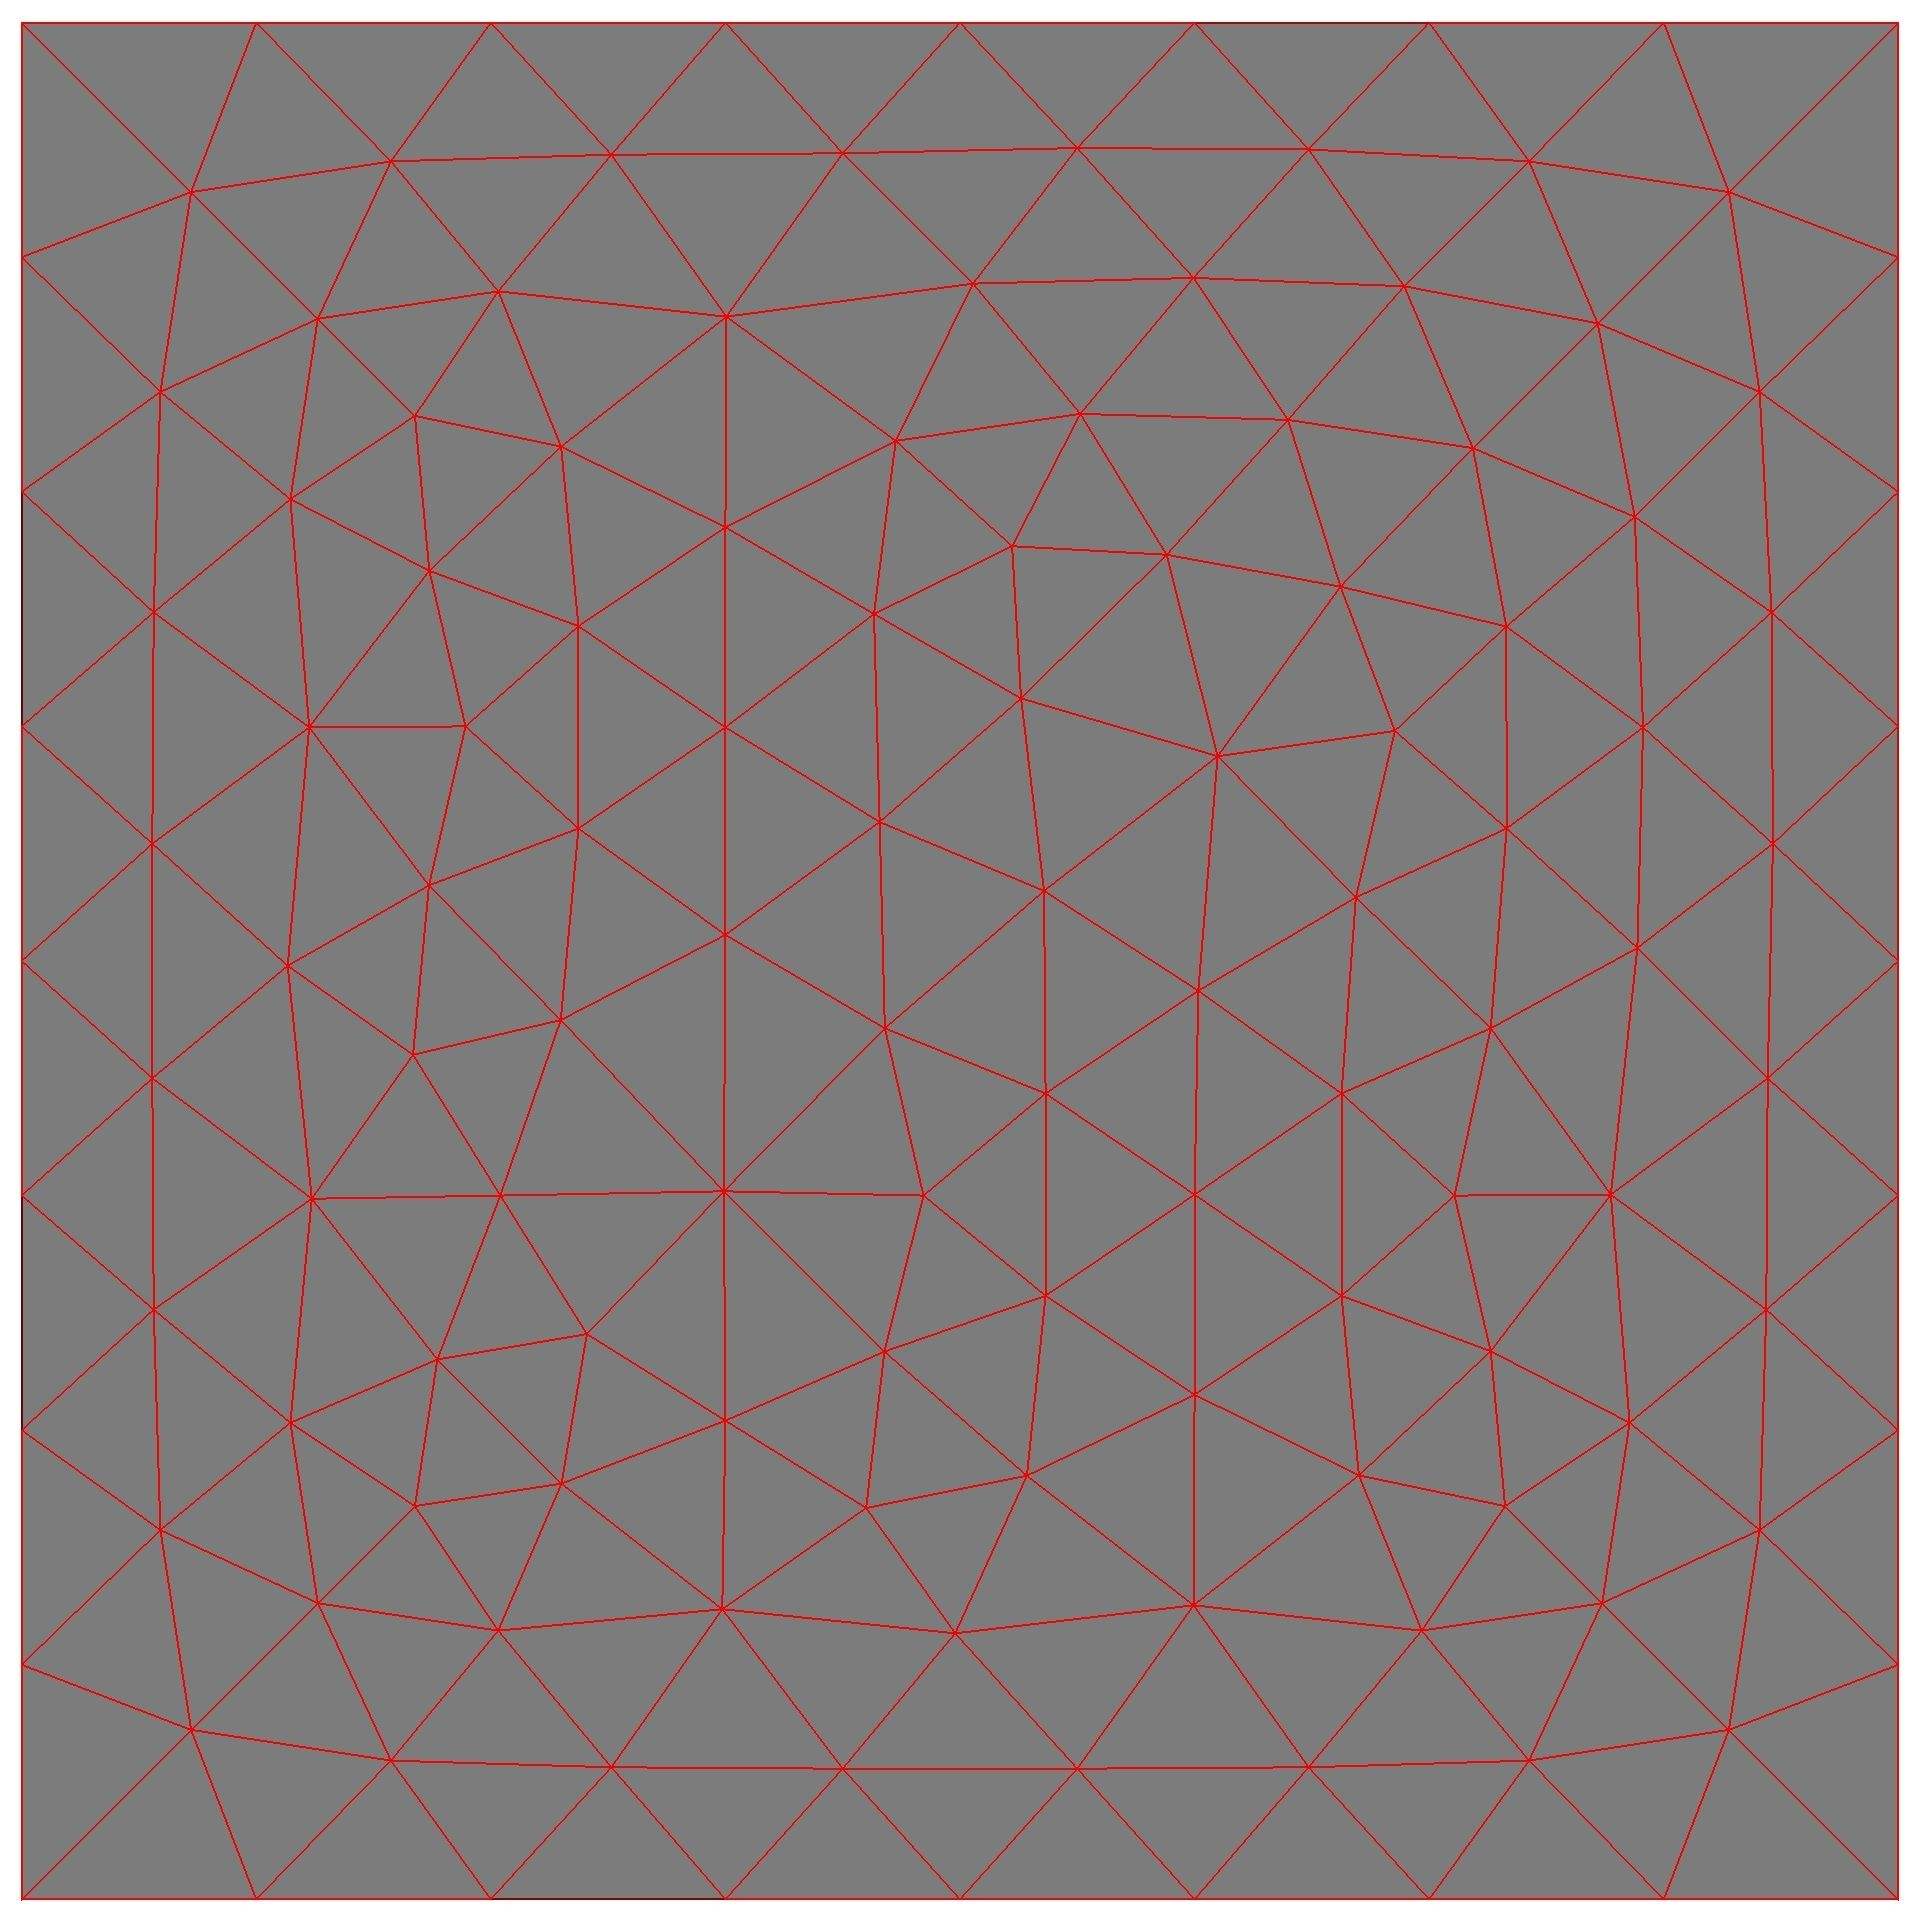
\includegraphics[width=0.45\textwidth]{figures/remesh_cube.jpg}}
    \caption{Example of isotropic remeshing of a face of a cube\label{fig:cube_remesh}}
\end{figure}

Once the area around the landing site is remeshed, the preceding shape reconstruction scheme is applied to those area to develop a high-fidelity topological map. 

\subsection{Numerical Example}

The proposed schemes for landing site selection and refinement are applied to Castalia.

%\section{Numerical Examples}\label{sec:reconstruction_examples}

% TODO Add more plots from dissertation. All the uncertainty and volume plots
% TODO Show examples with the other asteroids
% TODO Mention that the software to do this is available online?

\paragraph{Castalia Landing Site Selection}

With an appropriate shape estimate, the spacecraft can autonomously transition from a shape reconstruction to a landing mode.
Based on the shape estimate we seek to determine the best location to land. 
In reality, any landing site selection would be based on a wide variety of factors and constraints, however we highlight a few which can be determined autonomously and from the shape estimate.
The first metric is related to the surface slope which is computed using the completed shape estimate and~\cref{eq:surface_slope}.
Areas which violate the slope constraint of \( \phi < \SI{5}{\degree} \) are excluded from further consideration.
\begin{figure}[htbp]
    \centering
    \subcaptionbox{Surface slope of Castalia\label{fig:surface_slope_castalia}}{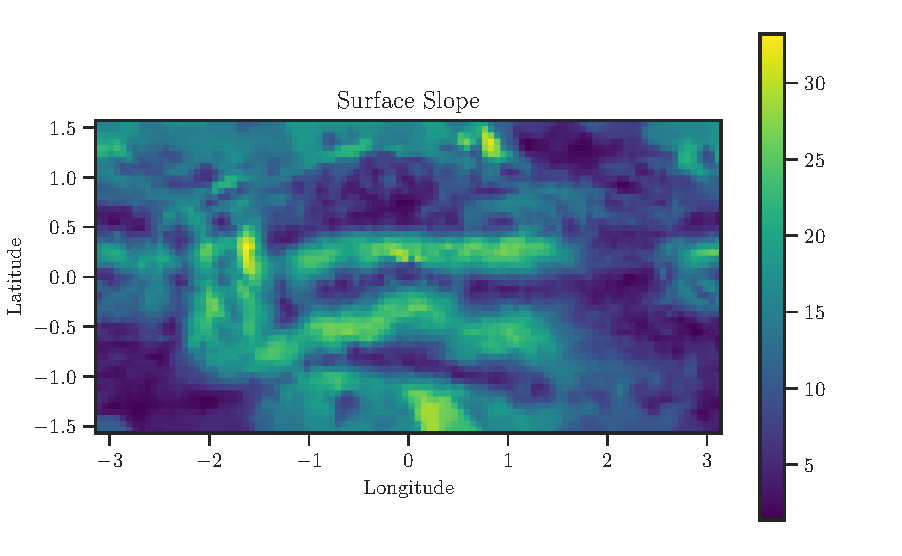
\includegraphics[width=0.5\textwidth]{figures/dynamic_exploration/castalia/refine/slope.pdf}}%
    \subcaptionbox{Masked surface slope with areas \( \phi > \SI{5}{\degree}\) excluded\label{fig:surface_slope_castalia_masked}}{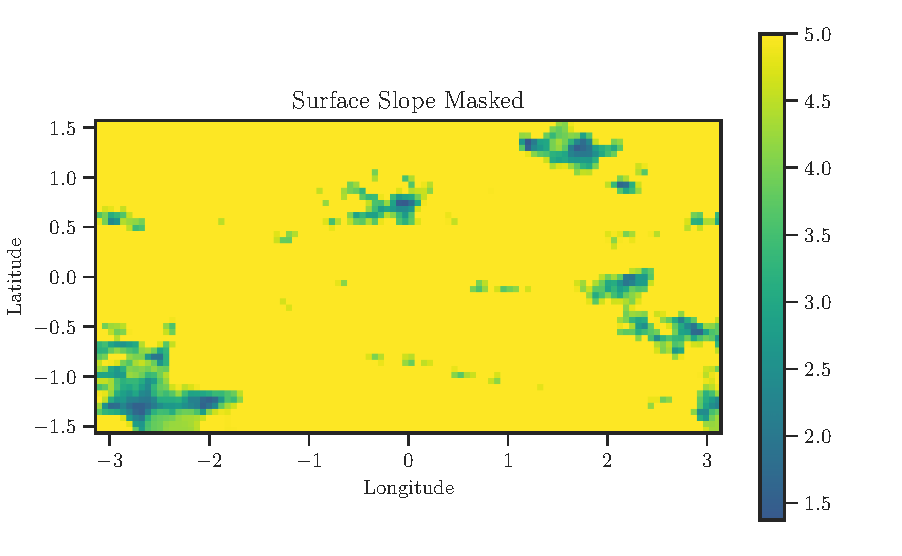
\includegraphics[width=0.5\textwidth,keepaspectratio]{figures/dynamic_exploration/castalia/refine/slope_masked.pdf}}
    \caption{Surface slope of asteroid Castalia\label{fig:surface_slope_castalia_both}}
\end{figure}

The next metric is related to the distance from the current spacecraft position to all candidate landing sites on the surface.
We utilize~\cref{eq:geodesic_distance} to compute a distance metric to the surface.
Landing sites which are closer will be considered preferentially over those at a larger distance.
\Cref{fig:distance_castalia_both} shows a surface plot of the distance to the surface. 
The area immediately beneath the spacecraft has a small cost while those on the opposite side of the asteroid have a much larger cost.
\begin{figure}[htbp]
    \centering
    \subcaptionbox{Surface Distance to surface of Castalia\label{fig:surface_distance_castalia}}{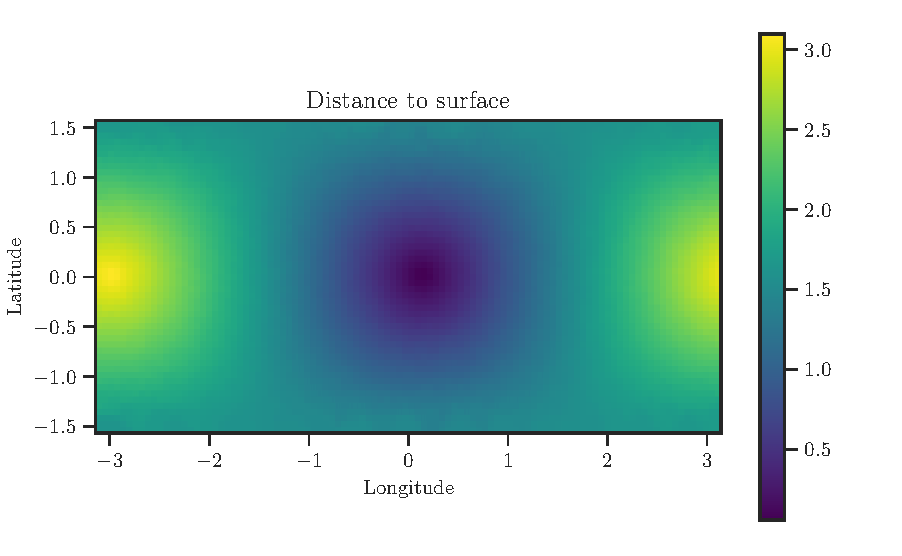
\includegraphics[width=0.5\textwidth]{figures/dynamic_exploration/castalia/refine/dist.pdf}}%
    \subcaptionbox{Masked distance to surface with areas \( \phi > \SI{5}{\degree}\) excluded\label{fig:surface_distance_castalia_masked}}{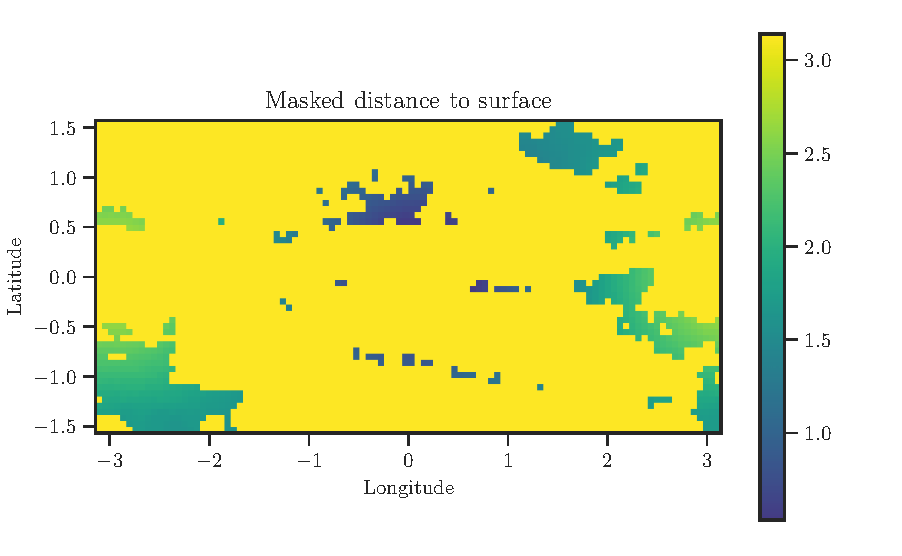
\includegraphics[width=0.5\textwidth,keepaspectratio]{figures/dynamic_exploration/castalia/refine/dist_masked.pdf}}
    \caption{Distance to surface of asteroid Castalia\label{fig:distance_castalia_both}}
\end{figure}
We can combine~\cref{fig:distance_castalia_both,fig:surface_slope_castalia_both} to determine the best landing site. 
The combination of the two is shown in~\cref{fig:landing_site_cost} with the desired landing site shown by the blue marker.
\begin{figure}[htbp]
    \centering
    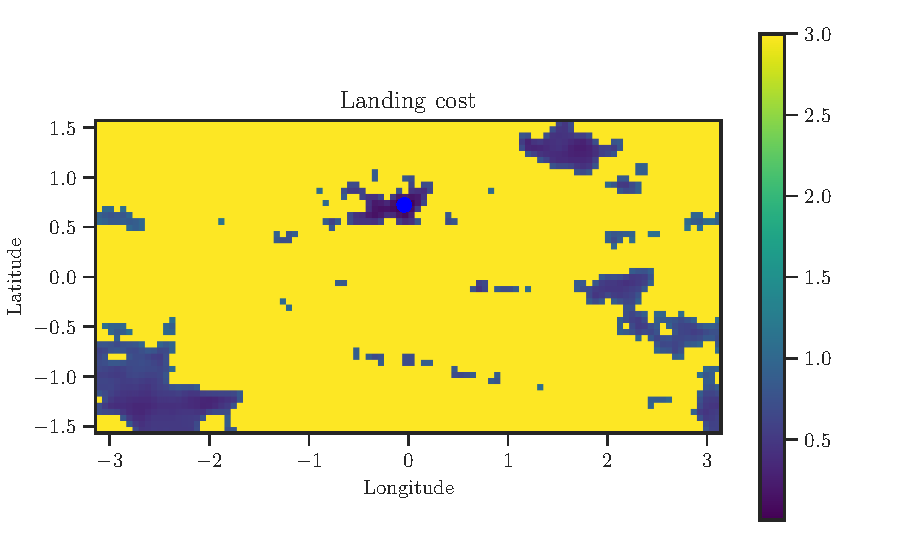
\includegraphics[width=0.75\textwidth,keepaspectratio]{figures/dynamic_exploration/castalia/refine/cost.pdf}
    \caption{Total cost for surface landing based on surface slope and distance\label{fig:landing_site_cost}}
\end{figure}
After selecting the appropriate landing site we then prepare for landing by collecting more measurements in the region around the landing area.


\paragraph{Castalia Landing Site Refinement}

%In order to demonstrate the multi resolution surface refinement we require a true shape model that contains small scale surface features.
%Here, we utilize the true radar shape model of asteroid 4769 Castalia.
%However, the shape model is not highly detailed as it does not contain small craters or surface features.
%In order to apply the landing refinement process we augment a small portion of the mesh with some additional features and utilize the mesh update scheme shown previously to update the surface.
%The augmented model of Castalia is shown in~\cref{fig:castalia_refinement}.
%\Cref{fig:castalia_refinement} shows that the increased resolution is required in order to reconstruct these small surface details.

One key benefit of an in-situ spacecraft is the ability to measure surface features at a much higher resolution than is possible from the ground. 
This detail provides a much higher fidelity data source than ground based measurements. 
In order to emulate this in the simulation we augment the shape model of Castalia with several small craters and outcroppings as shown in~\cref{fig:castalia_refinement}.
However, these small features would be difficult to capture with the current low resolution shape model of approximately \num{4000} faces.
The lower number of faces is useful for the evaluation of the polyhedron potential model, it is not ideal for the capture of minute surface features. 
As a result, we utilize the isotropic remeshing operation described previously to selectively increase the fidelity in the region about the desired landing site.

\Cref{fig:castalia_refine_density} shows that the vertex density increases by approximately an order of magnitude in region immediately surround the landing site.
\begin{figure}[htbp]
    \centering
    \subcaptionbox{Original vertex density of the initial shape estimate\label{fig:intial_vertex_density}}{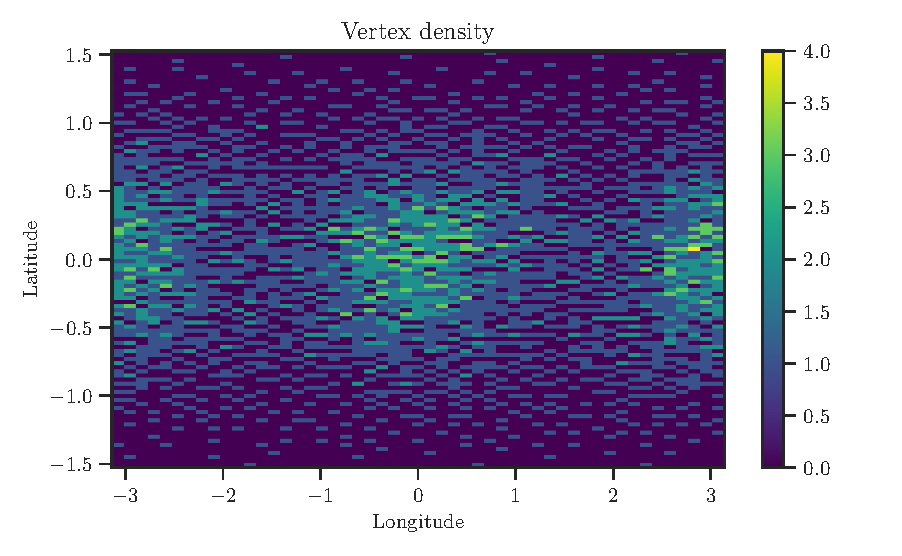
\includegraphics[width=0.5\textwidth]{figures/dynamic_exploration/castalia/refine/density.pdf}}%
    \subcaptionbox{Vertex density after refinement  around landing site\label{fig:refine_vertex_density}}{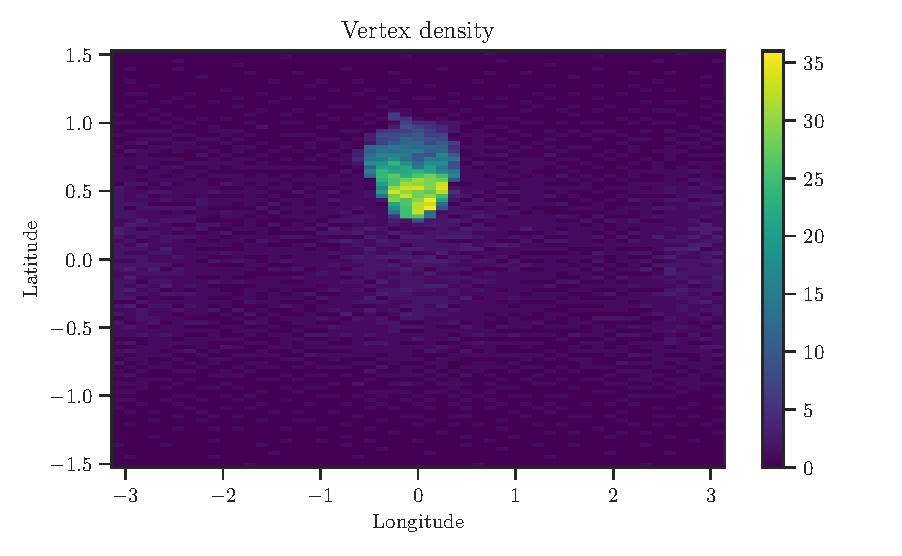
\includegraphics[width=0.5\textwidth]{figures/dynamic_exploration/castalia/land/density.pdf}}
    \caption{Vertex density before and after refinement at asteroid Castalia\label{fig:castalia_refine_density}}
\end{figure}

The increased number of faces and vertices in the landing area allows for the capture of the small surface features.
\Cref{fig:castalia_refinement} shows that given LIDAR measurements alone and the shape reconstruction algorithm that the small features are effectively estimated.
\begin{figure}[htbp]
    \centering
    \subcaptionbox{Augmented shape of Castalia with surface features\label{fig:orig_castalia}}{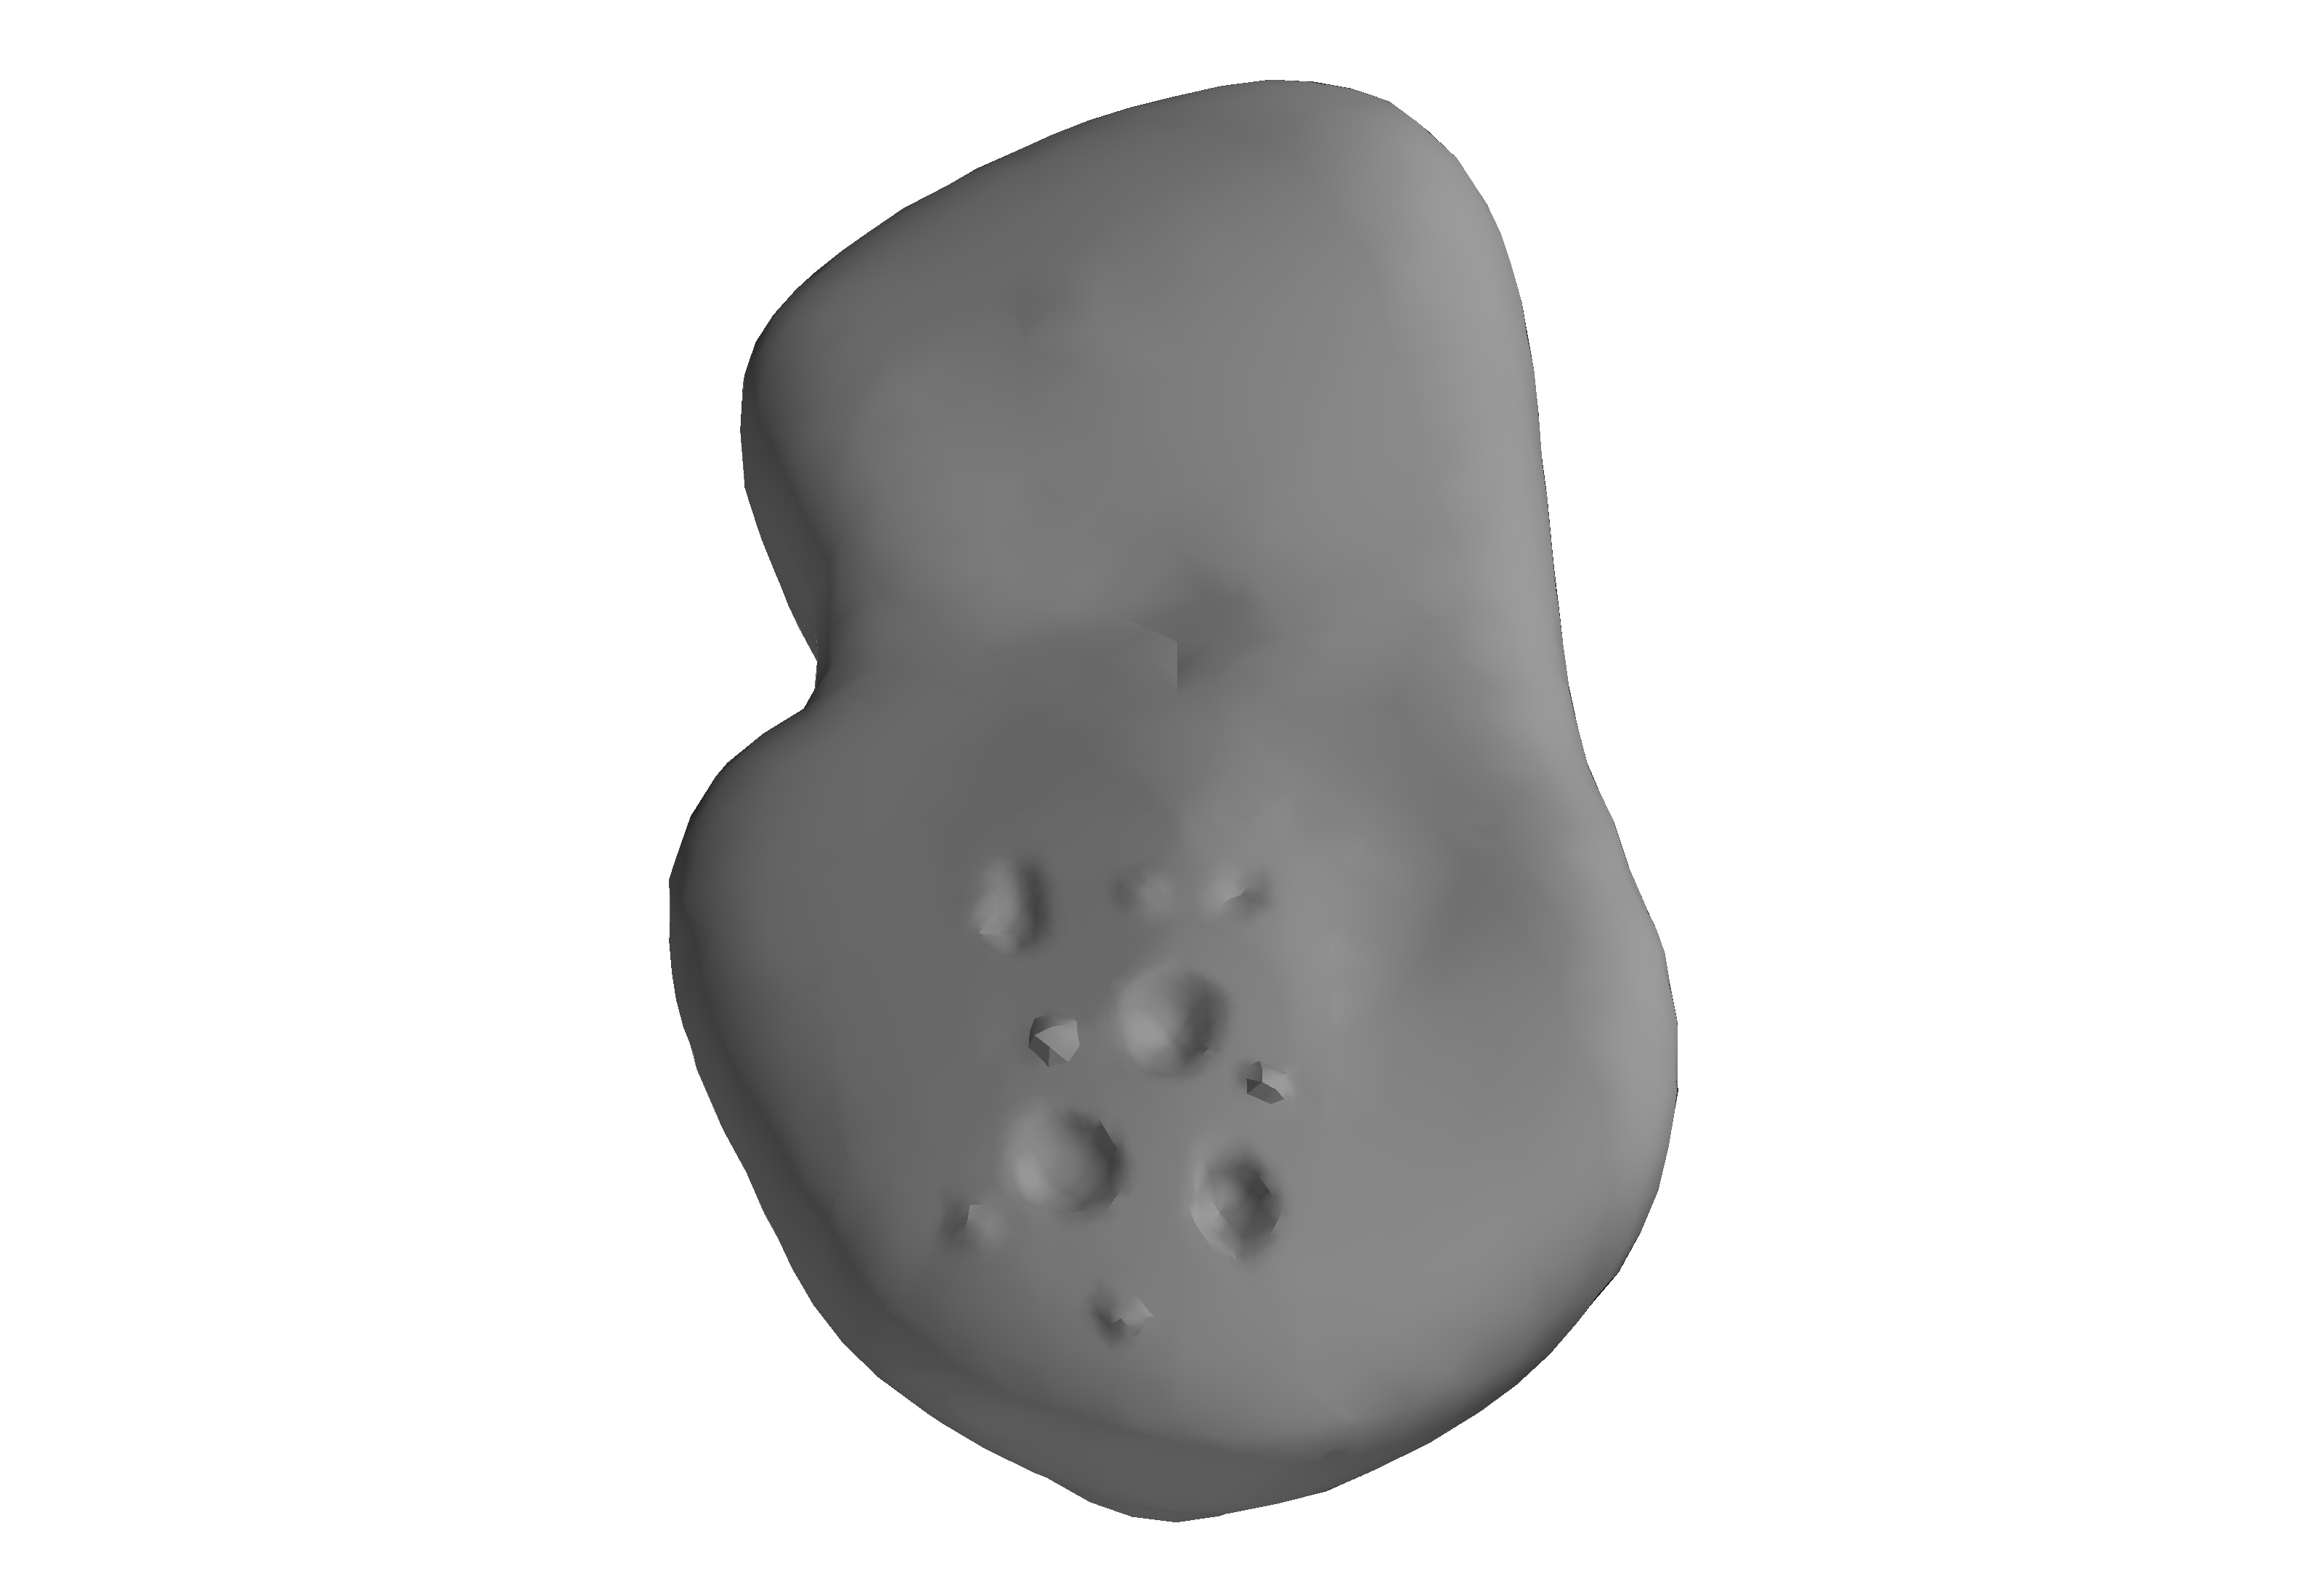
\includegraphics[trim={15cm 0 15cm 0},clip,keepaspectratio,height=0.3\textheight,width=0.5\textwidth]{figures/dynamic_exploration/castalia_bump_true.jpg}}%
    \subcaptionbox{Estimated shape model after measuring the surface\label{fig:bump_castalia}}{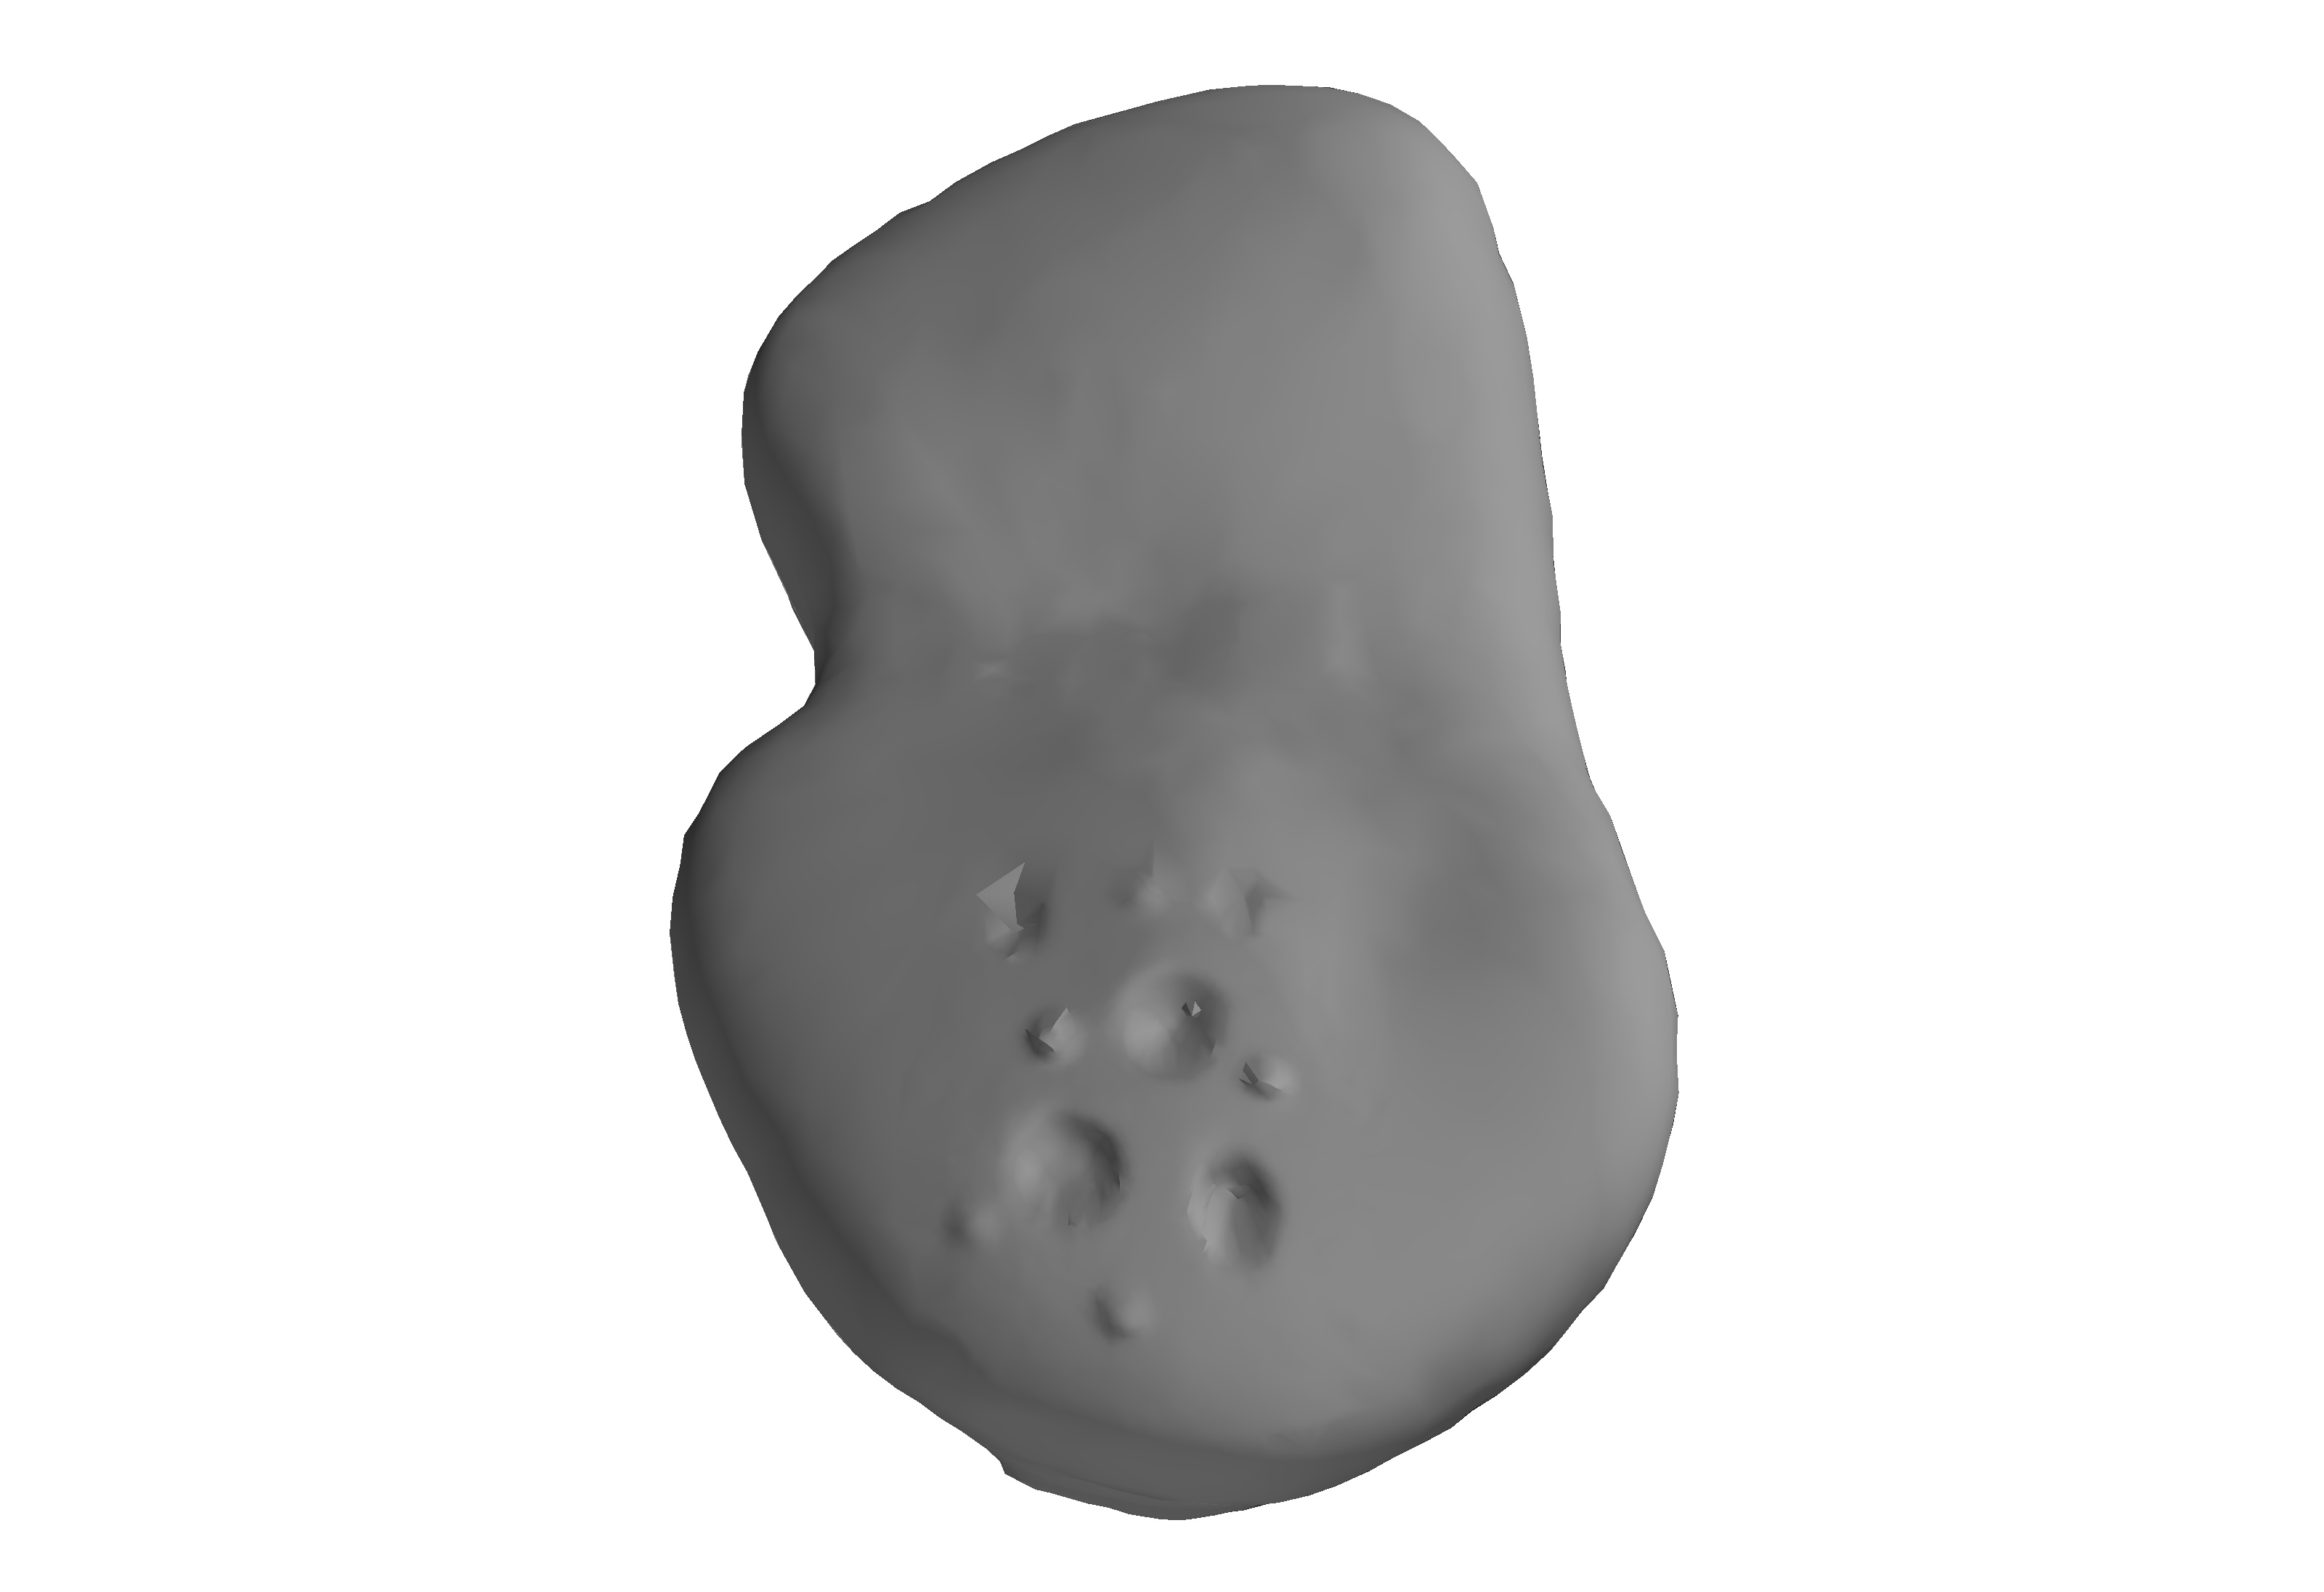
\includegraphics[trim={15cm 0 15cm 0},clip,keepaspectratio,height=0.3\textheight,width=0.5\textwidth]{figures/dynamic_exploration/castalia_bump_est.jpg}}
    \caption{Asteroid Castalia with augmented with additional surface features~\label{fig:castalia_refinement}}
\end{figure}

\paragraph{Castalia Vertical Descent}

The final phase of the simulation is to utilize the estimated shape model and vertically descend to the desired landing site. 
This is accomplished using the closed loop control of the vehicle and a trajectory which transitions from the home position to the surface over \SI{3600}{\second}.
The landing trajectory, using the estimated shape, is visualized in the asteroid frame in~\cref{fig:castalia_landing}.
During the vertical descent the vehicle is able to accurately track the desired trajectory using the estimated shape to compute the gravitational potential.
\begin{figure}[htbp]
    \centering
    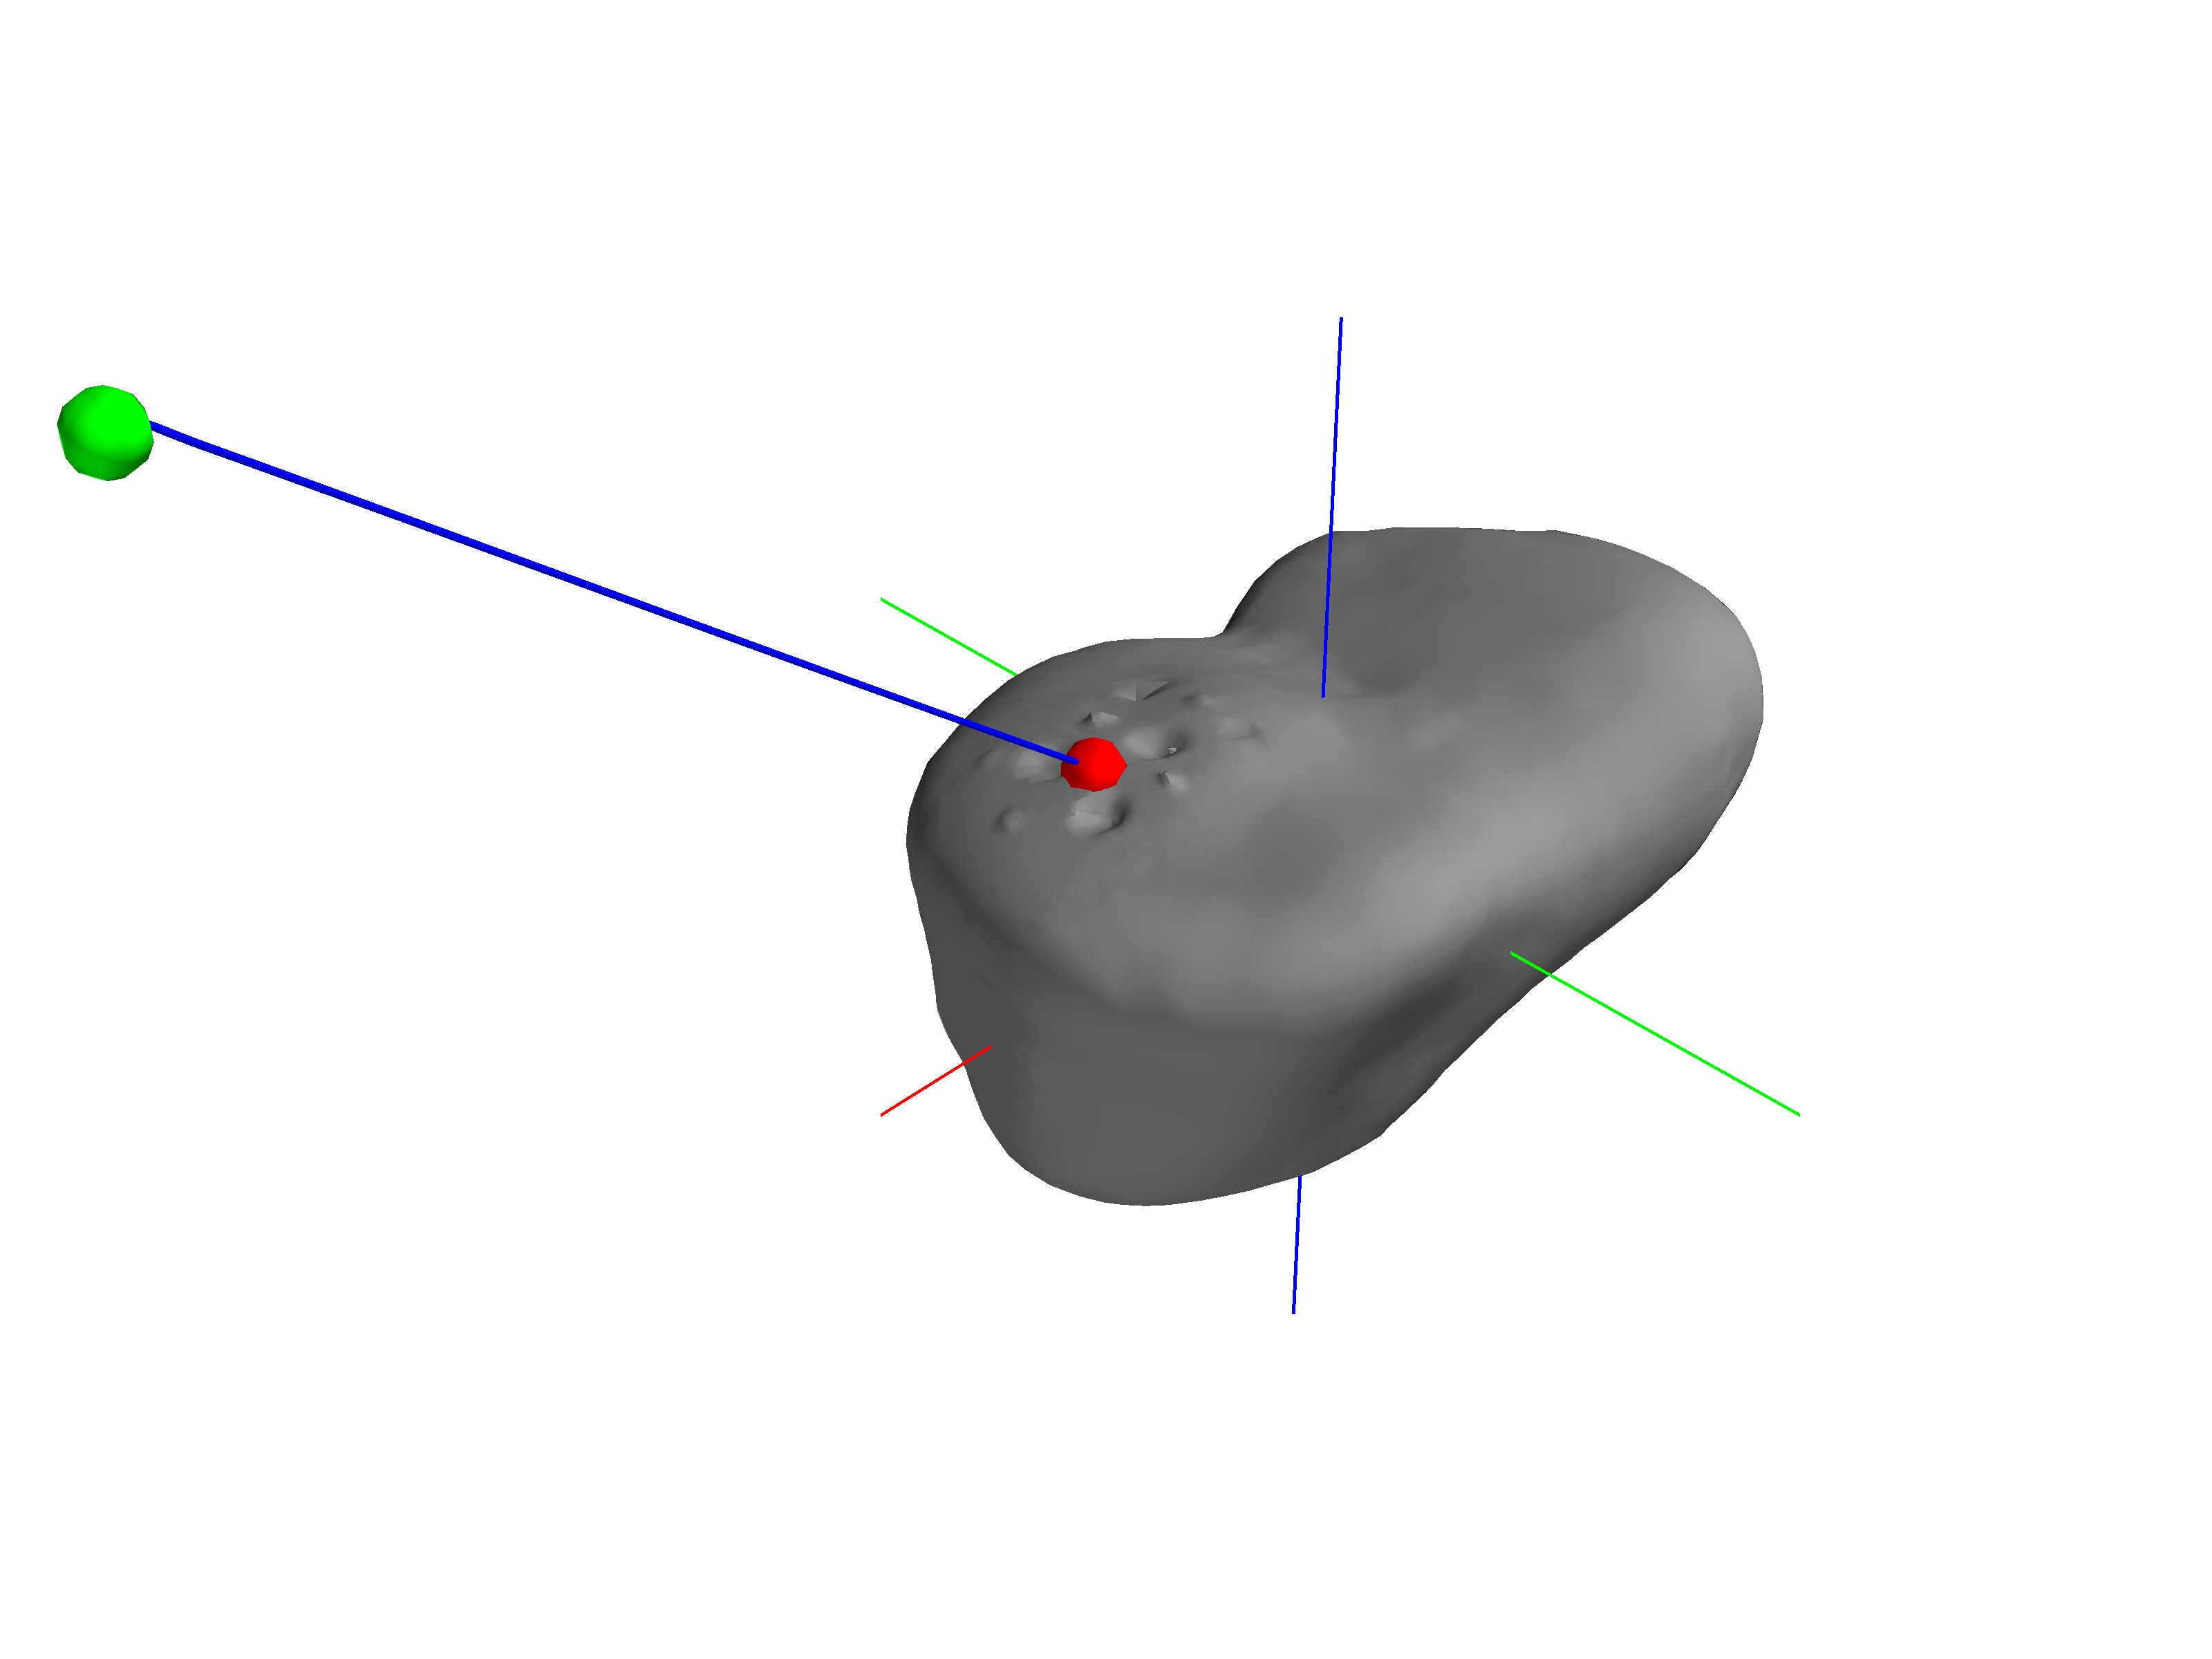
\includegraphics[width=0.8\textwidth]{figures/dynamic_exploration/castalia/land/asteroid_trajectory.jpg}
    \caption{Vertical descent onto 4769 Castalia~\label{fig:castalia_landing}}
\end{figure}

\todo{as the nonlinear controller is added, we may want to add more plots for tracking errors; we can add a link to videos}

\section{Conclusions}

This paper developed a Bayesian update scheme to reconstruct the shape of a small body from range measurements. 
The approach allows for a local update operation that is able to reconstruct the shape in real time. 
This is in contrast to standard shape reconstruction algorithms which operate over the entire surface and require signification computational resources.
Next, an optimal guidance scheme is derived which determines the desired state to best update the shape estimate. 
Finally, a mixed resolution shape representation is presented to allow for an increased fidelity in a specific region of the asteroid.
This allows for a much greater shape accuracy in a local area while avoiding the computational costs associated with a uniformly high resolution mesh.
This allows for a spacecraft to autonomously maneuver and reconstruct the shape of a small body without operator intervention.
Several numerical examples were presented which demonstrates the approach on a number of real asteroids.

Throughout this paper, it is considered that the position of the spacecraft relative the asteroid is available. 
Future works include integrating a localization technique with the proposed shape reconstruction scheme such that the relative location and the shape model are estimated simultaneously.


%\section*{Appendix}

%An Appendix, if needed, appears \textbf{before} research funding information and other acknowledgments.

%\section*{Funding Sources}

%Sponsorship information and acknowledgments of financial support should be included here. \textbf{Authors are responsible for accurately reporting funding data relevant to their research.} Please confirm that you have correctly entered \textbf{all sources} of funding and grant/award numbers \textbf{for all authors} in this section of your article. You will also be asked to select the appropriate funding organization from a drop-down menu in ScholarOne when you submit your manuscript. Be careful to choose the correct funder name, as organization names can be similar, and also be mindful to select sub-organizations within the registry hierarchy that are the actual funding sources, as appropriate, rather than choosing the name of the parent organization. Information provided in your manuscript must match the funding data entered in ScholarOne.

\section{Acknowledgement}
This research is supported in part by NSF under the grant CMMI-1335008.

\bibliography{library}


\end{document}
